\documentclass[ignorenonframetext,]{beamer}
\setbeamertemplate{caption}[numbered]
\setbeamertemplate{caption label separator}{: }
\setbeamercolor{caption name}{fg=normal text.fg}
\beamertemplatenavigationsymbolsempty
\usepackage{lmodern}
\usepackage{amssymb,amsmath}
\usepackage{ifxetex,ifluatex}
\usepackage{fixltx2e} % provides \textsubscript
\ifnum 0\ifxetex 1\fi\ifluatex 1\fi=0 % if pdftex
  \usepackage[T1]{fontenc}
  \usepackage[utf8]{inputenc}
\else % if luatex or xelatex
  \ifxetex
    \usepackage{mathspec}
  \else
    \usepackage{fontspec}
  \fi
  \defaultfontfeatures{Ligatures=TeX,Scale=MatchLowercase}
\fi
\usetheme[]{CambridgeUS}
\usecolortheme{beaver}
\usefonttheme{structurebold}
% use upquote if available, for straight quotes in verbatim environments
\IfFileExists{upquote.sty}{\usepackage{upquote}}{}
% use microtype if available
\IfFileExists{microtype.sty}{%
\usepackage{microtype}
\UseMicrotypeSet[protrusion]{basicmath} % disable protrusion for tt fonts
}{}
\newif\ifbibliography
\hypersetup{
            pdftitle={Geodaten - erster Teil},
            pdfauthor={Jan-Philipp Kolb},
            pdfborder={0 0 0},
            breaklinks=true}
\urlstyle{same}  % don't use monospace font for urls
\usepackage{color}
\usepackage{fancyvrb}
\newcommand{\VerbBar}{|}
\newcommand{\VERB}{\Verb[commandchars=\\\{\}]}
\DefineVerbatimEnvironment{Highlighting}{Verbatim}{commandchars=\\\{\}}
% Add ',fontsize=\small' for more characters per line
\usepackage{framed}
\definecolor{shadecolor}{RGB}{248,248,248}
\newenvironment{Shaded}{\begin{snugshade}}{\end{snugshade}}
\newcommand{\KeywordTok}[1]{\textcolor[rgb]{0.13,0.29,0.53}{\textbf{#1}}}
\newcommand{\DataTypeTok}[1]{\textcolor[rgb]{0.13,0.29,0.53}{#1}}
\newcommand{\DecValTok}[1]{\textcolor[rgb]{0.00,0.00,0.81}{#1}}
\newcommand{\BaseNTok}[1]{\textcolor[rgb]{0.00,0.00,0.81}{#1}}
\newcommand{\FloatTok}[1]{\textcolor[rgb]{0.00,0.00,0.81}{#1}}
\newcommand{\ConstantTok}[1]{\textcolor[rgb]{0.00,0.00,0.00}{#1}}
\newcommand{\CharTok}[1]{\textcolor[rgb]{0.31,0.60,0.02}{#1}}
\newcommand{\SpecialCharTok}[1]{\textcolor[rgb]{0.00,0.00,0.00}{#1}}
\newcommand{\StringTok}[1]{\textcolor[rgb]{0.31,0.60,0.02}{#1}}
\newcommand{\VerbatimStringTok}[1]{\textcolor[rgb]{0.31,0.60,0.02}{#1}}
\newcommand{\SpecialStringTok}[1]{\textcolor[rgb]{0.31,0.60,0.02}{#1}}
\newcommand{\ImportTok}[1]{#1}
\newcommand{\CommentTok}[1]{\textcolor[rgb]{0.56,0.35,0.01}{\textit{#1}}}
\newcommand{\DocumentationTok}[1]{\textcolor[rgb]{0.56,0.35,0.01}{\textbf{\textit{#1}}}}
\newcommand{\AnnotationTok}[1]{\textcolor[rgb]{0.56,0.35,0.01}{\textbf{\textit{#1}}}}
\newcommand{\CommentVarTok}[1]{\textcolor[rgb]{0.56,0.35,0.01}{\textbf{\textit{#1}}}}
\newcommand{\OtherTok}[1]{\textcolor[rgb]{0.56,0.35,0.01}{#1}}
\newcommand{\FunctionTok}[1]{\textcolor[rgb]{0.00,0.00,0.00}{#1}}
\newcommand{\VariableTok}[1]{\textcolor[rgb]{0.00,0.00,0.00}{#1}}
\newcommand{\ControlFlowTok}[1]{\textcolor[rgb]{0.13,0.29,0.53}{\textbf{#1}}}
\newcommand{\OperatorTok}[1]{\textcolor[rgb]{0.81,0.36,0.00}{\textbf{#1}}}
\newcommand{\BuiltInTok}[1]{#1}
\newcommand{\ExtensionTok}[1]{#1}
\newcommand{\PreprocessorTok}[1]{\textcolor[rgb]{0.56,0.35,0.01}{\textit{#1}}}
\newcommand{\AttributeTok}[1]{\textcolor[rgb]{0.77,0.63,0.00}{#1}}
\newcommand{\RegionMarkerTok}[1]{#1}
\newcommand{\InformationTok}[1]{\textcolor[rgb]{0.56,0.35,0.01}{\textbf{\textit{#1}}}}
\newcommand{\WarningTok}[1]{\textcolor[rgb]{0.56,0.35,0.01}{\textbf{\textit{#1}}}}
\newcommand{\AlertTok}[1]{\textcolor[rgb]{0.94,0.16,0.16}{#1}}
\newcommand{\ErrorTok}[1]{\textcolor[rgb]{0.64,0.00,0.00}{\textbf{#1}}}
\newcommand{\NormalTok}[1]{#1}
\usepackage{longtable,booktabs}
\usepackage{caption}
% These lines are needed to make table captions work with longtable:
\makeatletter
\def\fnum@table{\tablename~\thetable}
\makeatother
\usepackage{graphicx,grffile}
\makeatletter
\def\maxwidth{\ifdim\Gin@nat@width>\linewidth\linewidth\else\Gin@nat@width\fi}
\def\maxheight{\ifdim\Gin@nat@height>\textheight0.8\textheight\else\Gin@nat@height\fi}
\makeatother
% Scale images if necessary, so that they will not overflow the page
% margins by default, and it is still possible to overwrite the defaults
% using explicit options in \includegraphics[width, height, ...]{}
\setkeys{Gin}{width=\maxwidth,height=\maxheight,keepaspectratio}

% Prevent slide breaks in the middle of a paragraph:
\widowpenalties 1 10000
\raggedbottom

\AtBeginPart{
  \let\insertpartnumber\relax
  \let\partname\relax
  \frame{\partpage}
}
\AtBeginSection{
  \ifbibliography
  \else
    \let\insertsectionnumber\relax
    \let\sectionname\relax
    \frame{\sectionpage}
  \fi
}
\AtBeginSubsection{
  \let\insertsubsectionnumber\relax
  \let\subsectionname\relax
  \frame{\subsectionpage}
}

\setlength{\parindent}{0pt}
\setlength{\parskip}{6pt plus 2pt minus 1pt}
\setlength{\emergencystretch}{3em}  % prevent overfull lines
\providecommand{\tightlist}{%
  \setlength{\itemsep}{0pt}\setlength{\parskip}{0pt}}
\setcounter{secnumdepth}{0}

\title{Geodaten - erster Teil}
\author{Jan-Philipp Kolb}
\date{11 Oktober 2018}

\begin{document}
\frame{\titlepage}

\begin{frame}{Das Thema Geodatenlandschaft}


\includegraphics{figure/BildRatSWDBericht.png}

\end{frame}

\begin{frame}[fragile]{R-Pakete - Zum Download von Geo-Information}

\begin{block}{\href{https://sites.google.com/site/davidkahle/ggmap}{Das
Paket \texttt{ggmap}}}

\begin{itemize}
\tightlist
\item
  David Kahle and Hadley Wickham: \texttt{ggmap} - Spatial Visualization
  with \texttt{ggplot2}
\end{itemize}

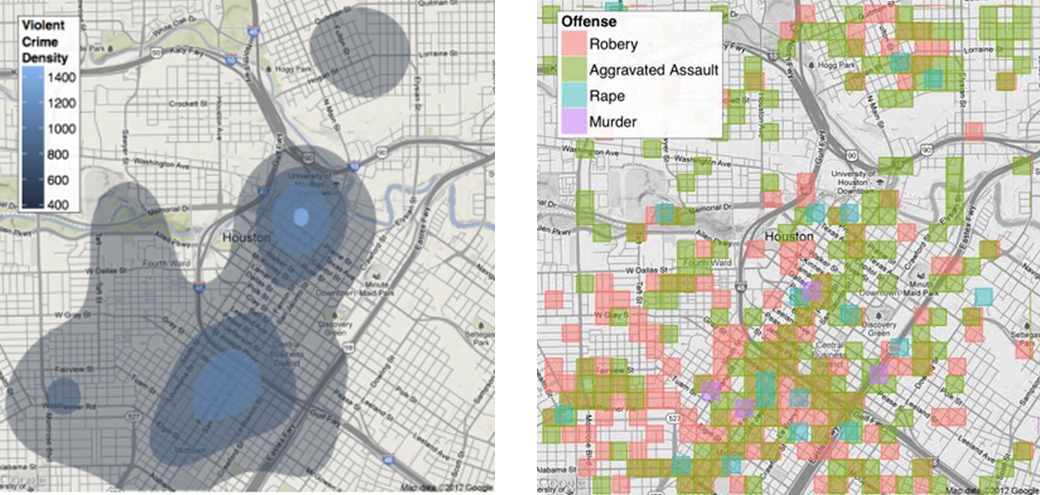
\includegraphics{figure/Rgeopackages.PNG}

\end{block}

\end{frame}

\begin{frame}{\href{http://blog.revolutionanalytics.com/2012/07/making-beautiful-maps-in-r-with-ggmap.html}{Worum
geht es?}}

\begin{block}{Weine probieren im Napa Valley?}

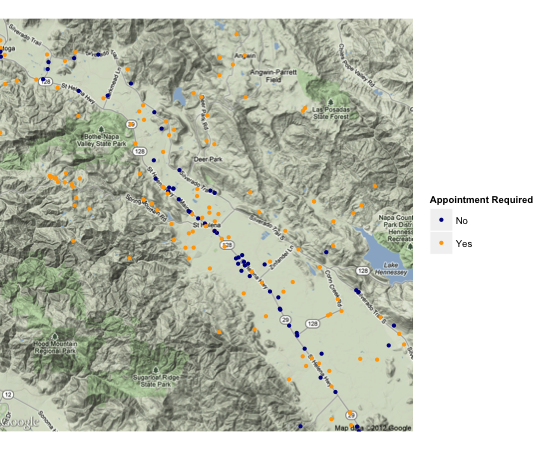
\includegraphics{figure/Wine_nappa.png}

\end{block}

\end{frame}

\begin{frame}{Ziel dieses Kurses}

\begin{block}{Vorgestellt werden:}

\begin{itemize}
\tightlist
\item
  Möglichkeiten für den Download, den Import, die Verarbeitung und die
  Visualisierung von Geodaten
\end{itemize}

\begin{itemize}
\item
  Die wichtigsten Programmierschnittstellen (APIs) um die Daten zu
  bekommen
\item
  R-Pakete um diese Daten zu verarbeiten und zu visualisieren
\end{itemize}

\end{block}

\end{frame}

\begin{frame}{Motivation}

\begin{itemize}
\tightlist
\item
  Sekundäranalyse für bestehenden Daten
\item
  Raumbezug herstellen/nutzen
\item
  Analysepotentiale der Geokodierung vorstellen
\item
  Verbindung von sozial- mit raumwissenschaftlichen Daten
\end{itemize}

\end{frame}

\begin{frame}{\href{http://de.slideshare.net/rheimann04/big-social-data-the-spatial-turn-in-big-data}{Laws
of Spatial Sience}}

\begin{block}{\href{https://en.wikipedia.org/wiki/Tobler's_first_law_of_geography}{Tobler's
law}}

\begin{quote}
everything is related to everything else, but near things are more
related than distant things.
\end{quote}

\end{block}

\begin{block}{\href{https://de.wikipedia.org/wiki/Spatial_turn}{Spatial
Turn}}

\begin{quote}
Spatial turn is a term used to describe an intellectual movement that
places emphasis on place and space in social science and the humanities.
\end{quote}

\end{block}

\end{frame}

\begin{frame}{Ergebnisse des Zensus 2011 zum
\href{https://www.zensus2011.de/SharedDocs/Aktuelles/Ergebnisse/DemografischeGrunddaten.html?nn=3065474}{\textbf{Download}}}


\includegraphics{figure/zensus2011_logo.jpg}

\begin{block}{Gemeindeebene}

\begin{itemize}
\tightlist
\item
  Bevölkerung nach Geschlecht, Altersgruppe, Familienstatus,
  Staatsangehörigkeit und Religion
\end{itemize}

\end{block}

\begin{block}{1 \(\text{km}^2\) Raster}

\begin{itemize}
\tightlist
\item
  Bevölkerung, Leerstandsquote, Wohnfläche und Haushaltsgröße
\end{itemize}

\end{block}

\begin{block}{100 \(\text{m}^2\) Raster}

Bevölkerung

\end{block}

\end{frame}

\begin{frame}{Zensus Ergebnisse}

Beispiel Anteil der Personen aus EU27 Land an Einwohnerzahl pro Gemeinde
in Oberfranken

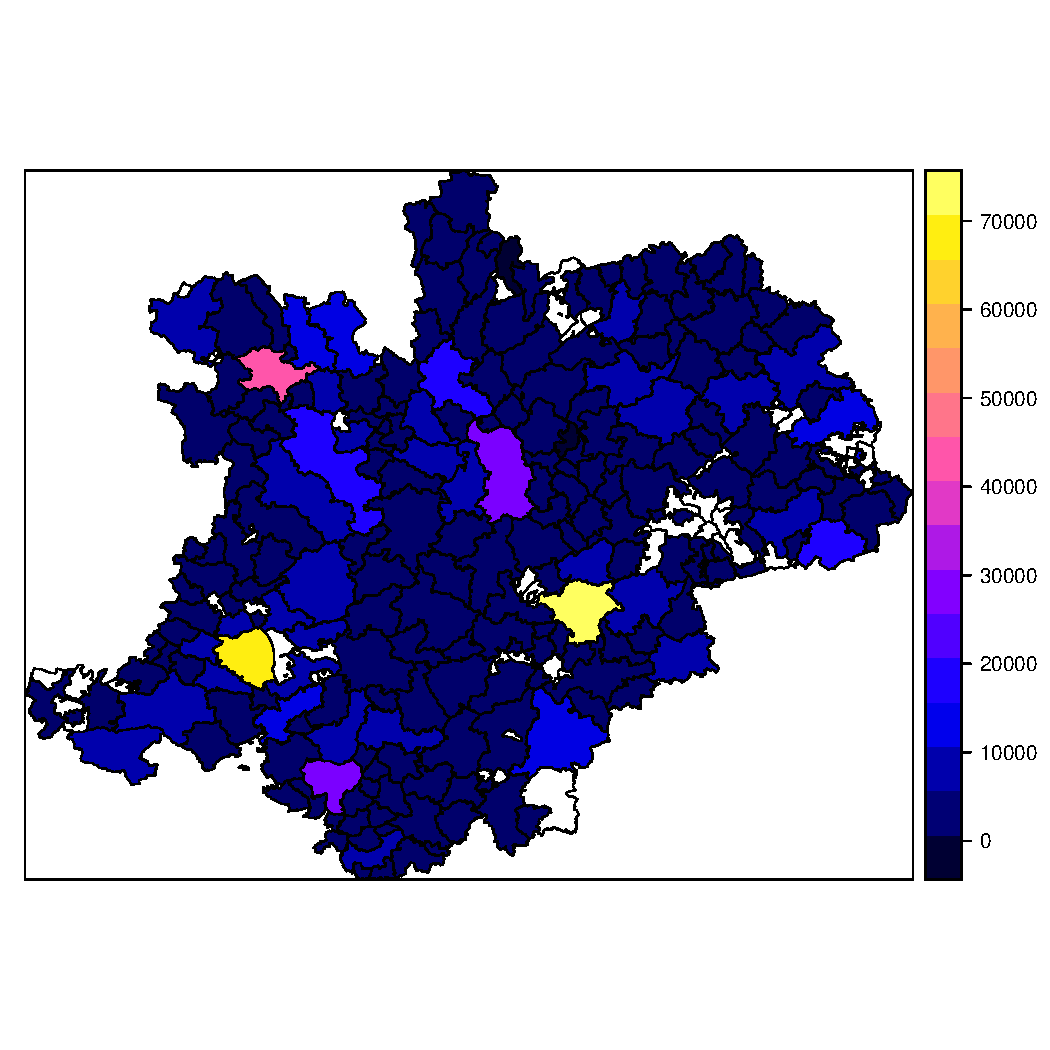
\includegraphics{figure/KRSBamberg_EWZ.pdf}

\end{frame}

\begin{frame}{Motivation - Warum die Darstellung in Karten}

\begin{itemize}
\item
  Darstellung in Karten ermöglicht besseres Verständnis bspw.
  sozialwissenschaftlicher Phänomene.
\item
  Attraktiver Output
\item
  Durch die INSPIRE Richtlinie und \emph{Collaborative Mapping} wächst
  der verfügbare Bestand an Geodaten.
\item
  Daten sind oft frei verfügbar im Internet (z.B. durch die Nutzung von
  APIs)
\item
  Die Daten sind allerdings oft wenig oder gar nicht strukturiert (z.B.
  Internet Dokumente), heterogen und
\item
  meistens nicht für die Nutzung zur räumlichen Visualisierung
  vorgesehen, beinhalten aber implizit geographische Informationen (Web
  2.0)
\item
  Oftmals sind wenig oder keine Metadaten vorhanden
\end{itemize}

\end{frame}

\begin{frame}{Openstreetmap Projekt}

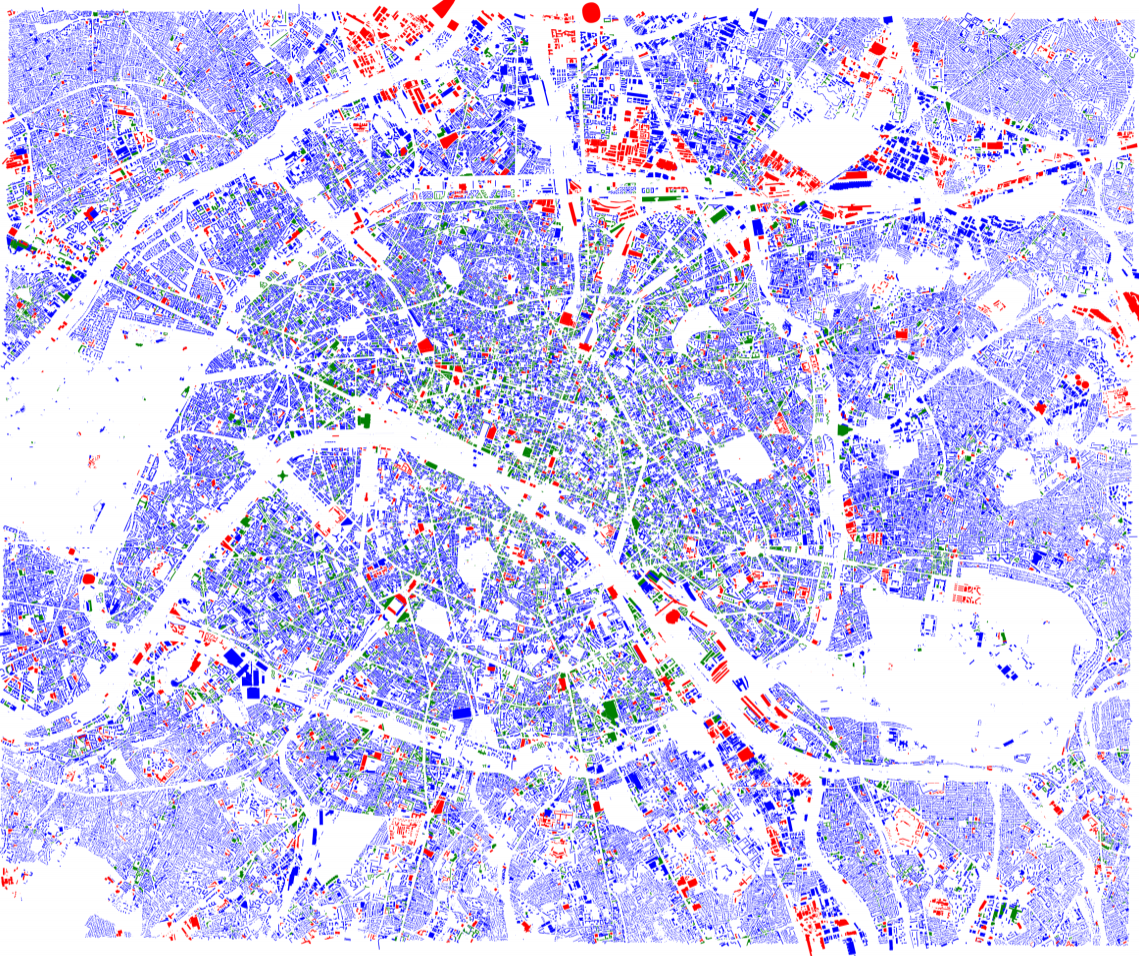
\includegraphics{figure/Buldings_Paris.PNG}

\end{frame}

\begin{frame}{Das Openstreetmap Projekt\ldots{}}

\begin{itemize}
\tightlist
\item
  Durch kollaboratives Mapping ist eine riesige Datenmenge zugänglich.
\item
  Viele Menschen tragen jeden Tag Informationen bei.
\item
  \ldots{} ermöglicht Zugang zu Big Data der Geographie.
\item
  Die wachsende Menge an Geodaten wird von Freiwilligen gesammelt oder
  über Crowd-sourcing gewonnen.
\end{itemize}

\end{frame}

\begin{frame}{Was ist das Ziel - Straßen in Berlin}

Dargestellt werden OpenStreetMap Daten, die mit der Overpass API
heruntergeladen wurden.

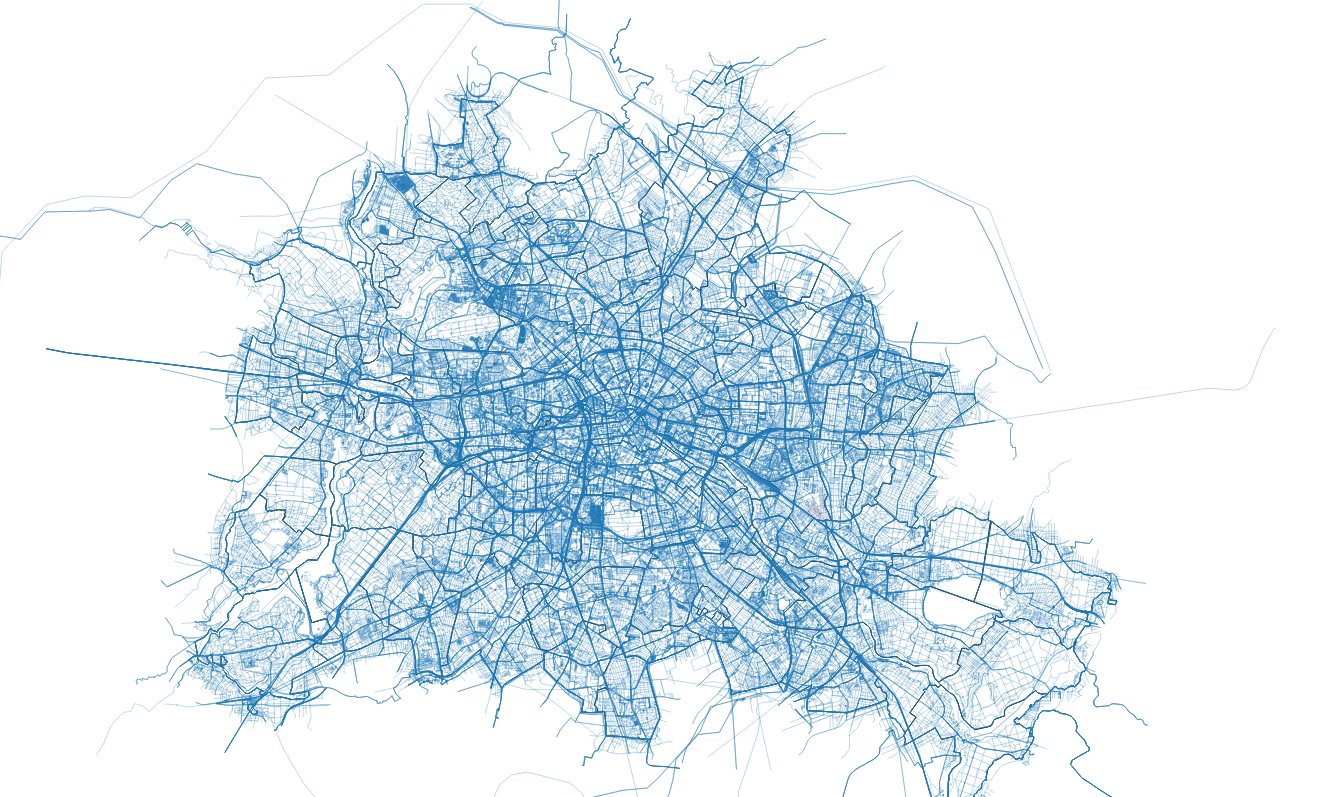
\includegraphics{figure/streets_Berlin2.png}

\end{frame}

\begin{frame}{Globale Muster der Straßeninfrastruktur}

\begin{block}{Studie von Johan Meijer, Mark AJ Huijbregts, Kees
Schotten, und Aafke Schipper}

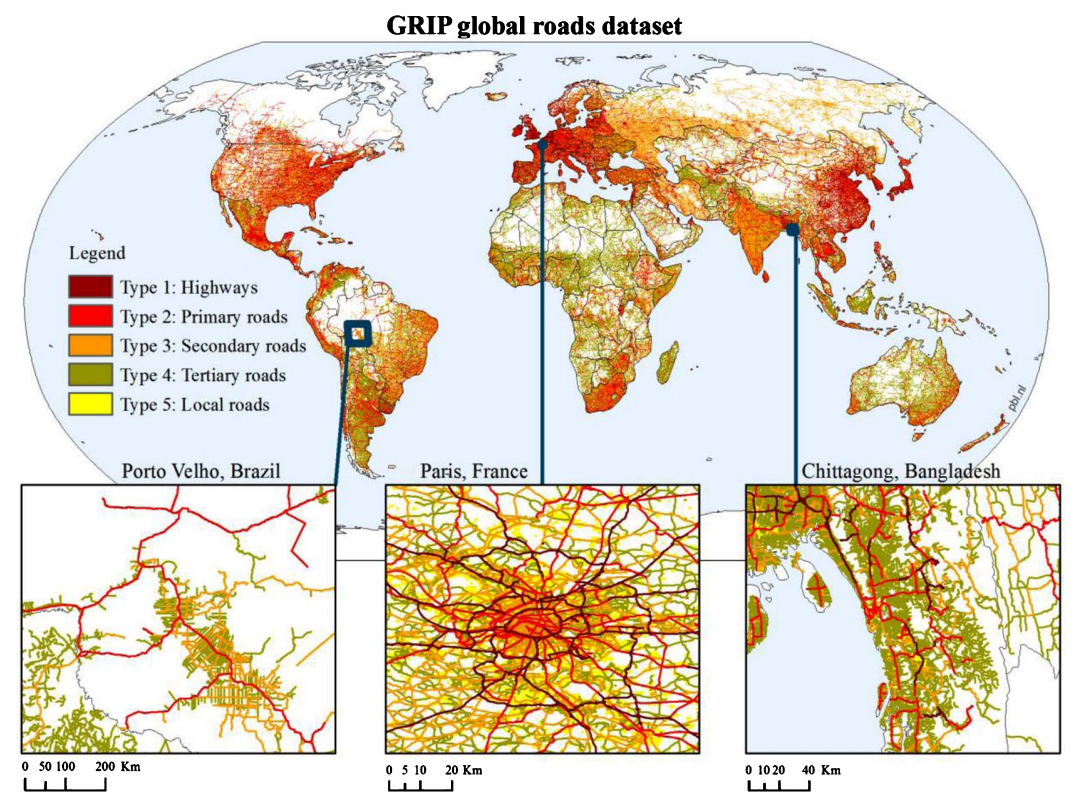
\includegraphics{figure/GRIP_globalroads.PNG}

\end{block}

\end{frame}

\begin{frame}{Links mit Beispielen}

\begin{itemize}
\item
  Shiny App zu
  \href{https://japhilko.shinyapps.io/Choropleths/}{\textbf{Indikatoren}}
  für Europa
\item
  Räumliche Visualisierung in den USA -
  \href{https://rpubs.com/Radcliffe/walmart}{\textbf{Walmarts in den
  USA}}
\item
  \href{http://www.nytimes.com/interactive/2014/09/03/us/the-race-gap-in-americas-police-departments.html?_r=0}{\textbf{Race
  Gap Police USA}} - \href{http://fivethirtyeight.com/}{\textbf{Wahl
  USA}}
\item
  Zeit Artikel zum Zustand der
  \href{http://detektor.fm/digital/datenjournalismus-interaktive-karte-zeigt-marode-deutsche-bahn-bruecken}{\textbf{Eisenbahnbrücken}}
\item
  \href{http://michael-hoerz.de/maps/berlin-bike/}{\textbf{Fahrradunfälle}}
  in Berlin
\item
  \href{http://interaktiv.morgenpost.de/beta-fussballkarte/\#7/51.258/10.756}{\textbf{Verteilung
  Fußballfans}}
\item
  \href{http://news.nationalgeographic.com/news/2014/07/140715-ocean-plastic-debris-trash-pacific-garbage-patch/}{\textbf{Plastiktüten
  im Meer}}
\end{itemize}

\begin{block}{Datenquellen:}

\begin{itemize}
\tightlist
\item
  Datensätze zu
  \href{https://www.pegelonline.wsv.de/gast/start}{\textbf{Pegelständen}}
  in Deutschland
\item
  Viele Datensätze auf \href{http://driven-by-data.net/}{\textbf{driven
  by data}}
\end{itemize}

\end{block}

\begin{block}{Resourcen}

\begin{itemize}
\tightlist
\item
  Andreas Plank -
  \href{http://www.chironomidaeproject.com/fileadmin/downloads/Formeln_in_R.pdf}{\textbf{Grafiken
  und Statistik in R}}
\end{itemize}

\end{block}

\end{frame}

\begin{frame}[fragile]{Inhalt dieses Abschnitts}

Arten von räumlichen Daten:

\begin{itemize}
\tightlist
\item
  \href{https://www.nceas.ucsb.edu/~frazier/RSpatialGuides/ggmap/ggmapCheatsheet.pdf}{\textbf{Straßenkarten}}
\item
  \href{http://www.mostlymuppet.com/tag/maps/}{\textbf{Satelliten
  Bilder}}
\item
  \href{http://gis.stackexchange.com/questions/3083/what-makes-a-map-beautiful/45518\#45518}{\textbf{Physische
  Daten und Karten}}
\item
  \href{http://www.designfaves.com/2014/03/abstracted-maps-reveal-cities-personalities}{\textbf{Abstrakte
  Karten}}
\item
  \ldots{}
\end{itemize}

Das R-paket
\href{http://journal.r-project.org/archive/2013-1/kahle-wickham.pdf}{\textbf{\texttt{ggmap}}}
wird im folgenden genutzt um verschiedene Kartentypen darzustellen.

Mit
\href{http://www.inside-r.org/packages/cran/ggmap/docs/qmap}{\textbf{\texttt{qmap}}}
kann man eine schnelle Karte erzeugen.

\end{frame}

\begin{frame}[fragile]{Installieren des Paketes}

\begin{itemize}
\tightlist
\item
  Zur Erstellung der Karten brauchen wir das Paket \texttt{ggmap}:
\end{itemize}

\begin{Shaded}
\begin{Highlighting}[]
\NormalTok{devtools}\OperatorTok{::}\KeywordTok{install_github}\NormalTok{(}\StringTok{"dkahle/ggmap"}\NormalTok{)}
\NormalTok{devtools}\OperatorTok{::}\KeywordTok{install_github}\NormalTok{(}\StringTok{"hadley/ggplot2"}\NormalTok{)}
\KeywordTok{install.packages}\NormalTok{(}\StringTok{"ggmap"}\NormalTok{)}
\end{Highlighting}
\end{Shaded}

\end{frame}

\begin{frame}[fragile]{Paket ggmap - Hallo Welt}

\begin{itemize}
\tightlist
\item
  Um das Paket zu laden verwenden wir den Befehl \texttt{library}
\end{itemize}

\begin{Shaded}
\begin{Highlighting}[]
\KeywordTok{library}\NormalTok{(ggmap)}
\end{Highlighting}
\end{Shaded}

Und schon kann die erste Karte erstellt werden:

\begin{Shaded}
\begin{Highlighting}[]
\KeywordTok{qmap}\NormalTok{(}\StringTok{"Mannheim"}\NormalTok{)}
\end{Highlighting}
\end{Shaded}

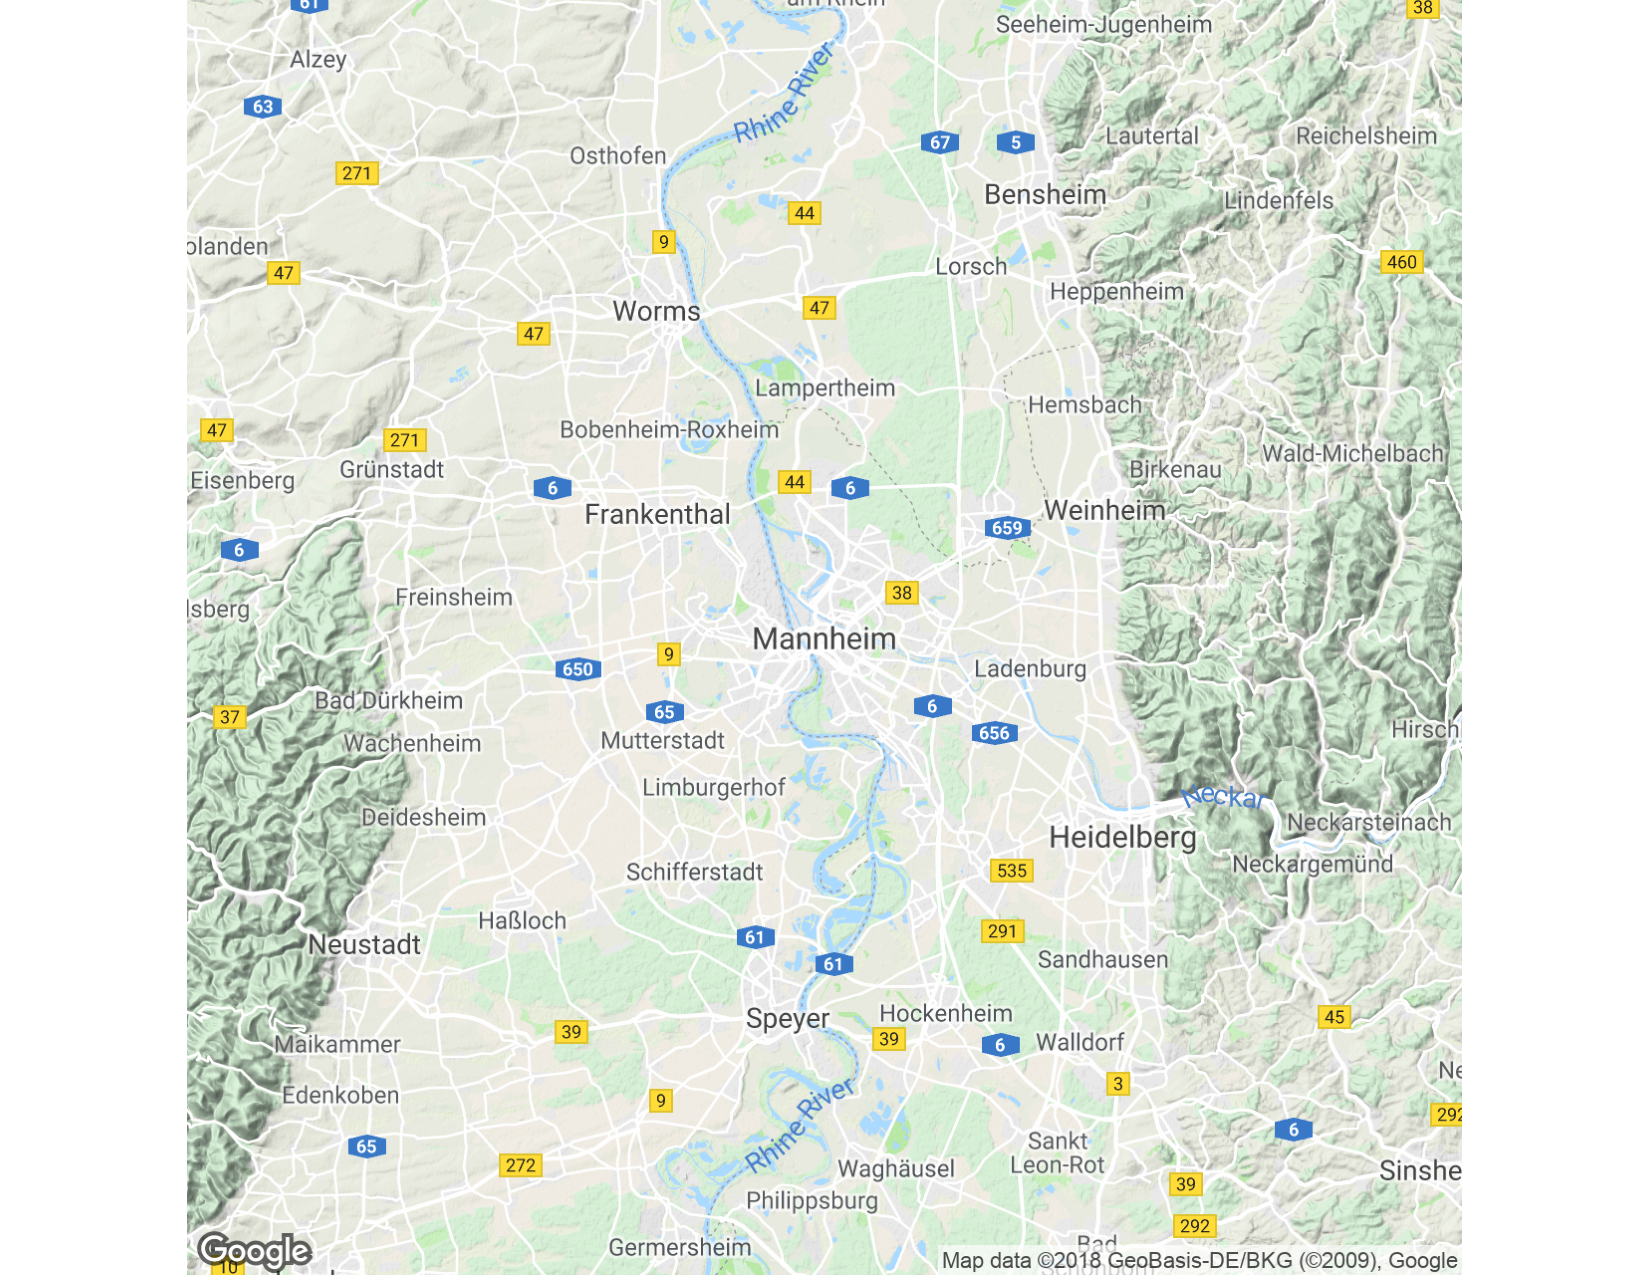
\includegraphics{figure/Mannheim_ggmap.pdf}

\end{frame}

\begin{frame}[fragile]{Karte für eine Sehenswürdigkeit}

\begin{Shaded}
\begin{Highlighting}[]
\KeywordTok{qmap}\NormalTok{(}\StringTok{"Berlin Brandenburger Tor"}\NormalTok{)}
\end{Highlighting}
\end{Shaded}

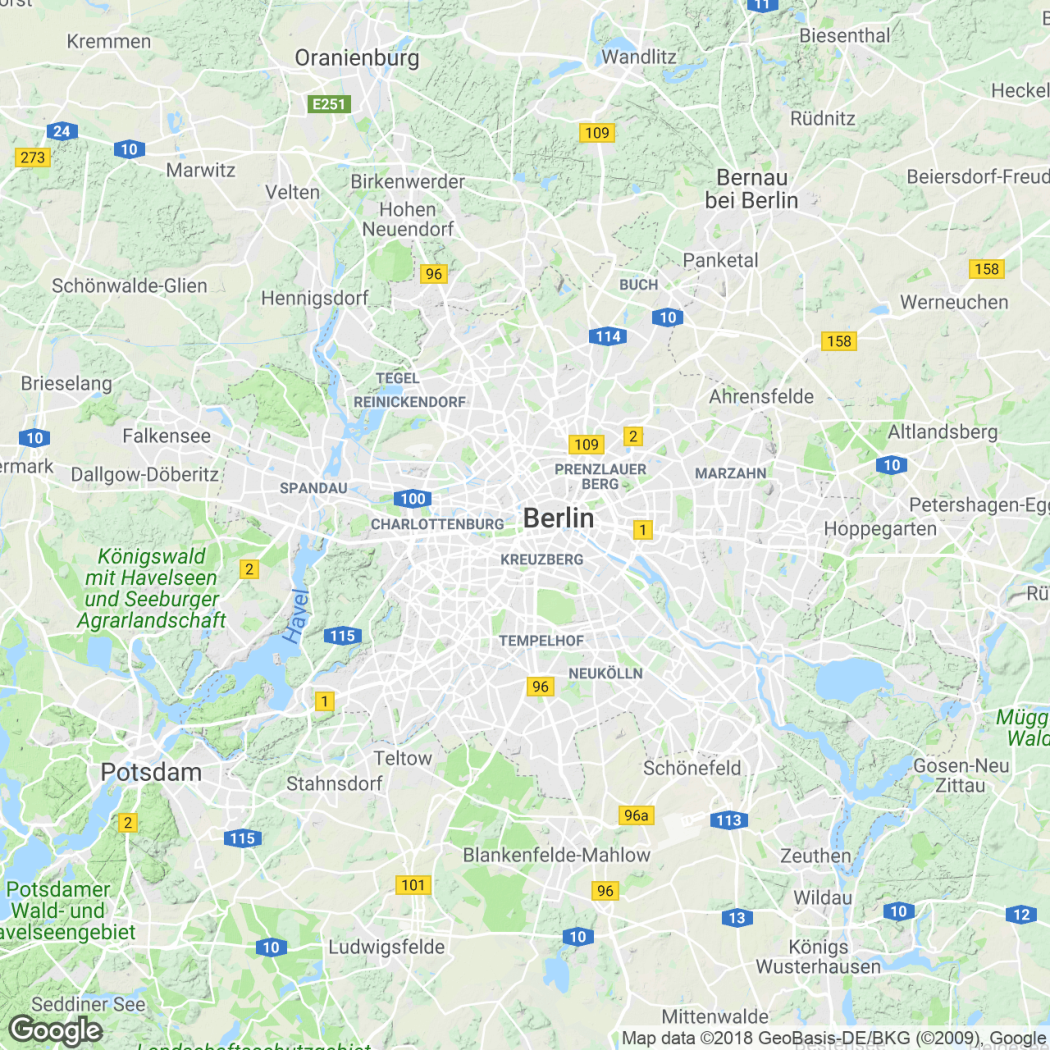
\includegraphics{figure/BBT_ggmap.pdf}

\end{frame}

\begin{frame}[fragile]{Karte für einen ganzen Staat}

\begin{Shaded}
\begin{Highlighting}[]
\KeywordTok{qmap}\NormalTok{(}\StringTok{"Germany"}\NormalTok{)}
\end{Highlighting}
\end{Shaded}

\begin{itemize}
\tightlist
\item
  Wir brauchen ein anderes \emph{zoom level}
\end{itemize}

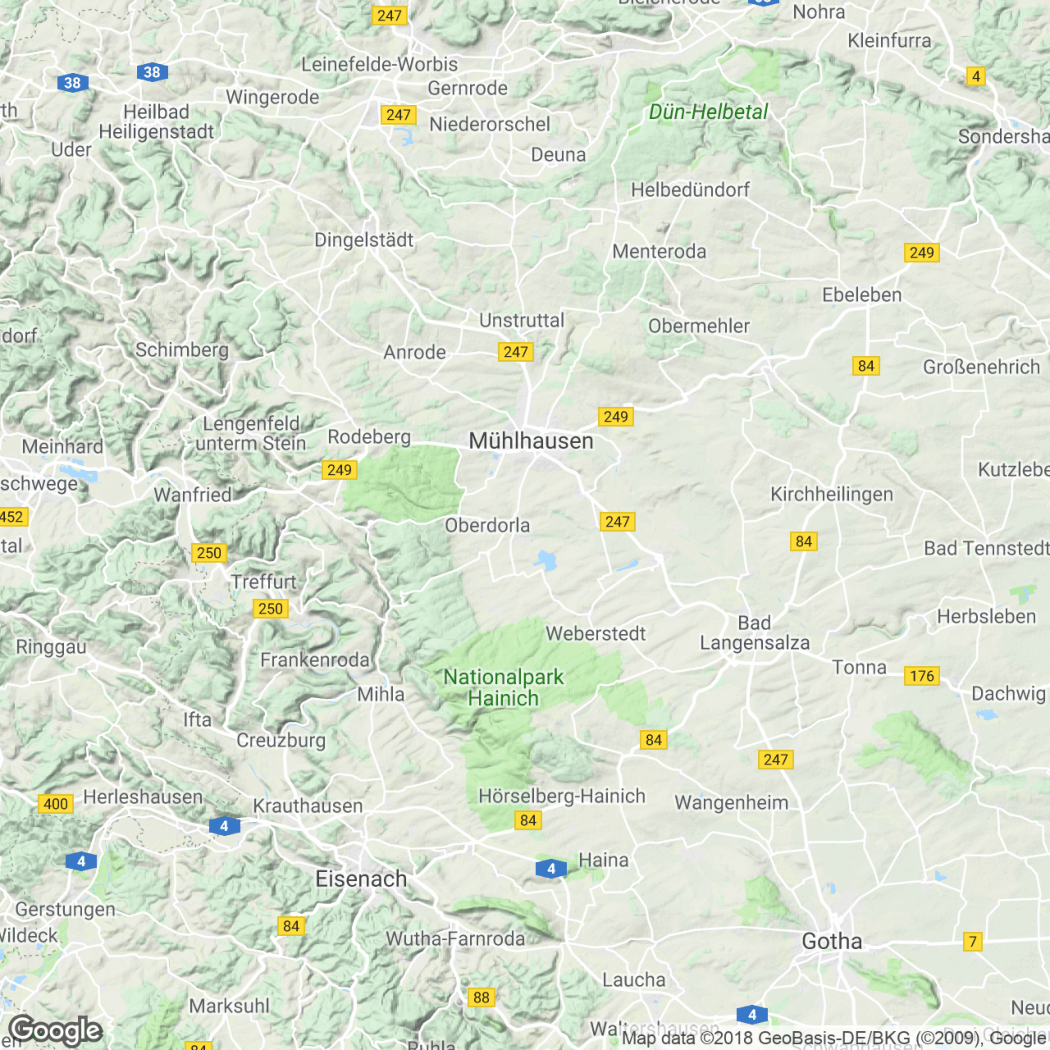
\includegraphics{figure/germany.pdf}

\end{frame}

\begin{frame}[fragile]{Ein anderes \emph{zoom level}}

\begin{itemize}
\tightlist
\item
  level 3 - Kontinent / level 10 - Stadt / level 21 - Gebäude
\end{itemize}

\begin{Shaded}
\begin{Highlighting}[]
\KeywordTok{qmap}\NormalTok{(}\StringTok{"England"}\NormalTok{, }\DataTypeTok{zoom =} \DecValTok{6}\NormalTok{)}
\end{Highlighting}
\end{Shaded}

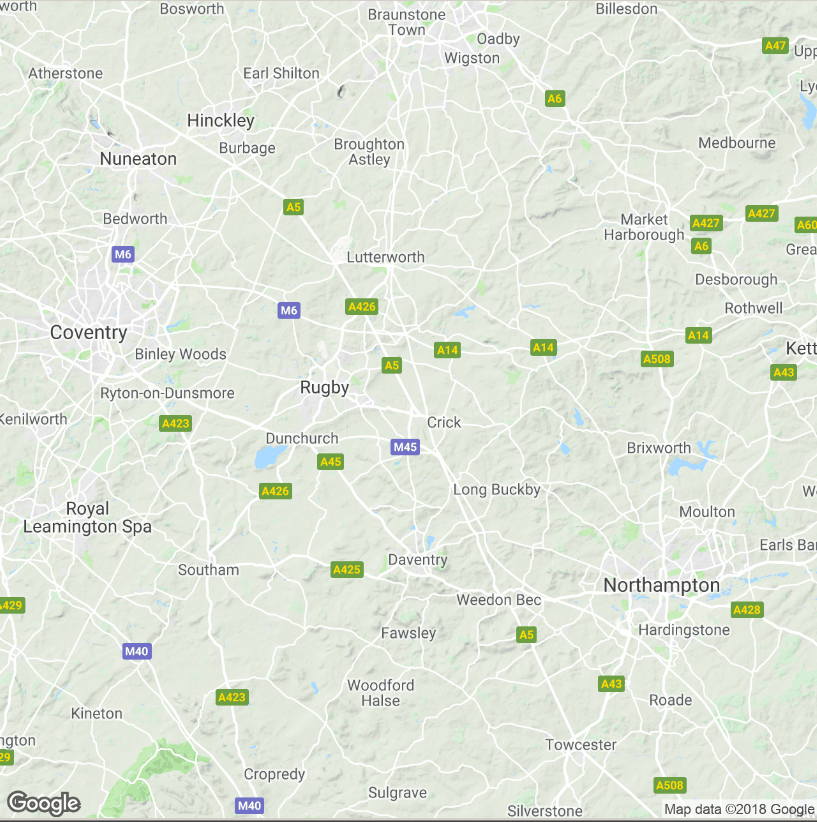
\includegraphics{figure/EnglandMap.PNG}

\end{frame}

\begin{frame}[fragile]{Hilfe bekommen wir mit dem Fragezeichen}

\begin{Shaded}
\begin{Highlighting}[]
\NormalTok{?qmap}
\end{Highlighting}
\end{Shaded}

Verschiedene Abschnitte in der Hilfe:

\begin{itemize}
\tightlist
\item
  Description
\item
  Usage
\item
  Arguments
\item
  Value
\item
  Author(s)
\item
  See Also
\item
  Examples
\end{itemize}

\end{frame}

\begin{frame}[fragile]{Ganz nah dran}

\begin{Shaded}
\begin{Highlighting}[]
\KeywordTok{qmap}\NormalTok{(}\StringTok{'Mannheim'}\NormalTok{, }\DataTypeTok{zoom =} \DecValTok{20}\NormalTok{)}
\end{Highlighting}
\end{Shaded}

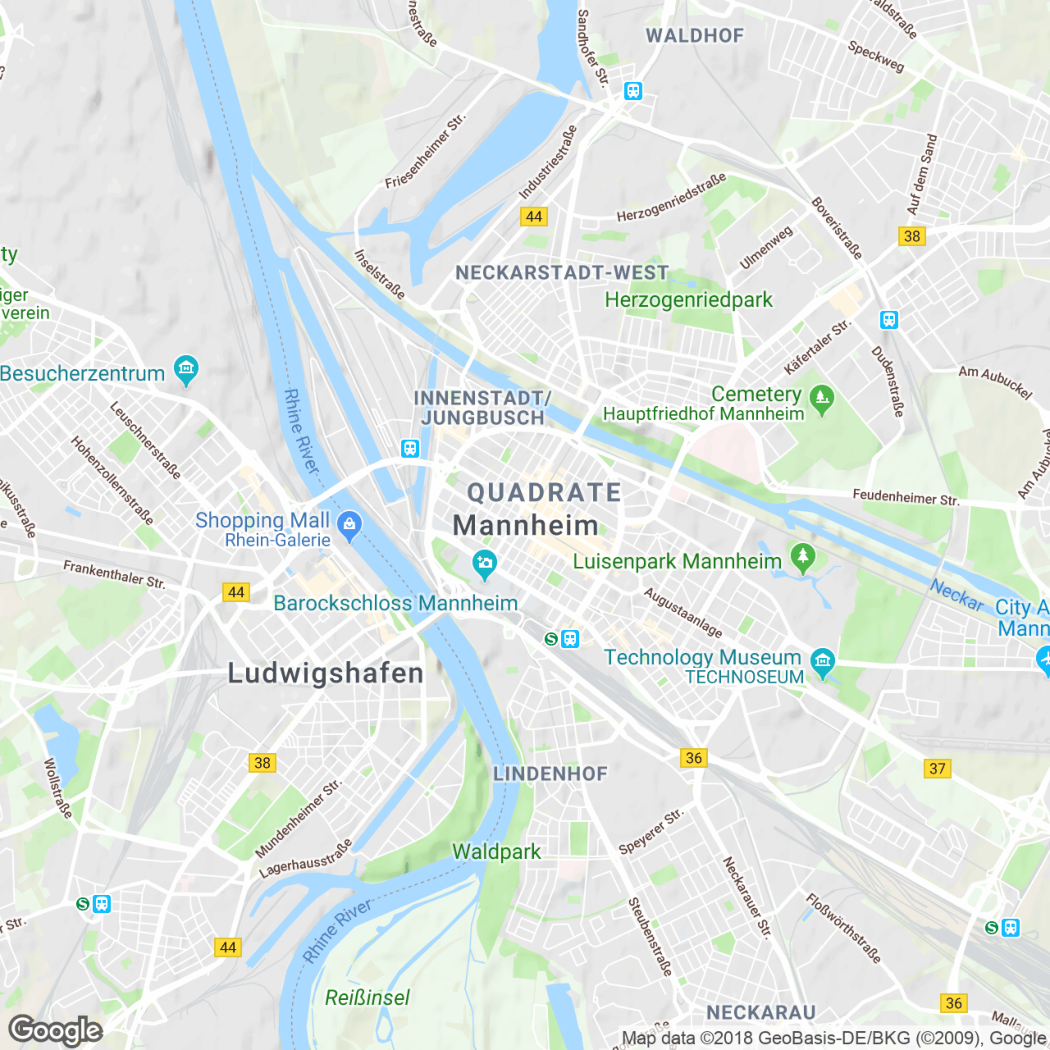
\includegraphics{figure/ham_map_z20.pdf}

\end{frame}

\begin{frame}[fragile]{\texttt{ggmap} - maptype satellite}

\begin{Shaded}
\begin{Highlighting}[]
\KeywordTok{qmap}\NormalTok{(}\StringTok{'Hamburg'}\NormalTok{, }\DataTypeTok{zoom =} \DecValTok{14}\NormalTok{, }\DataTypeTok{maptype=}\StringTok{"satellite"}\NormalTok{)}
\end{Highlighting}
\end{Shaded}

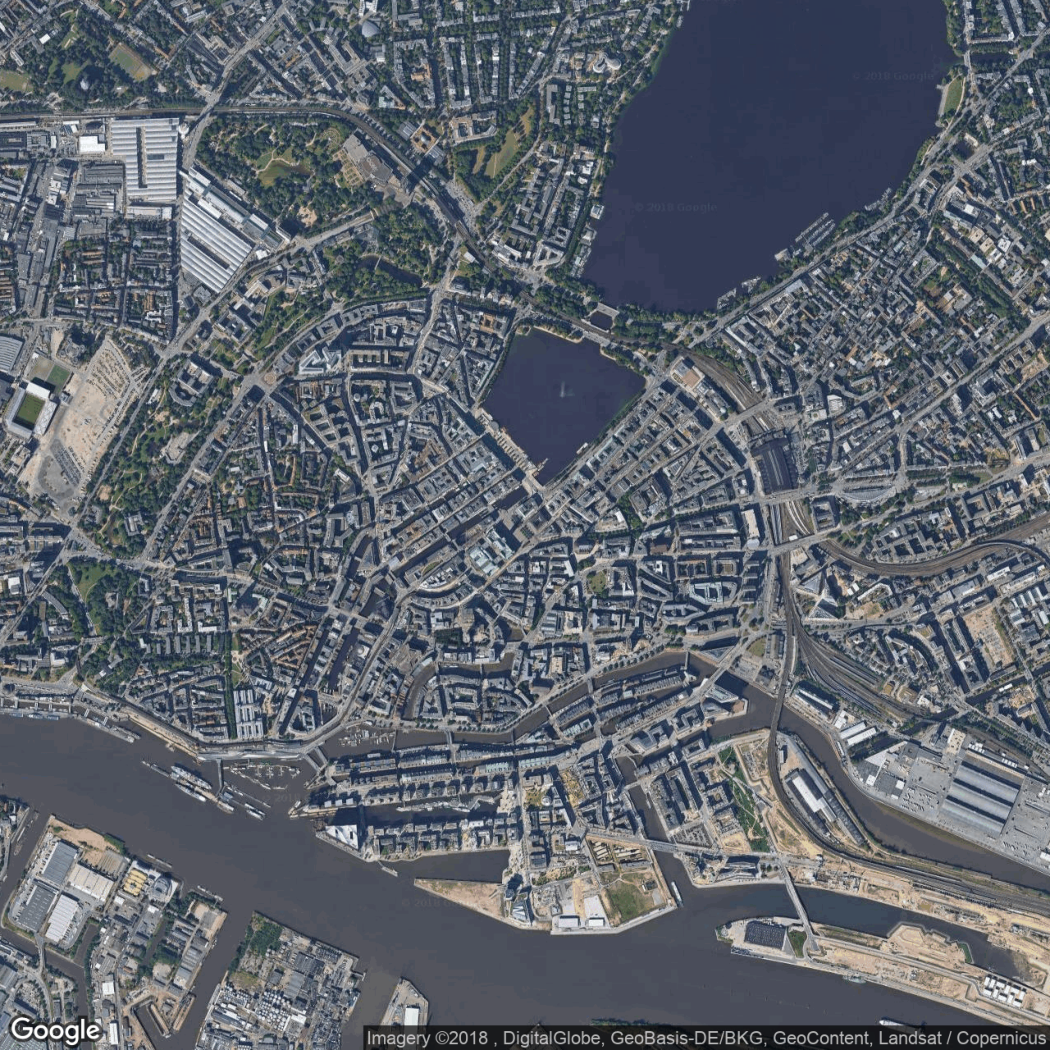
\includegraphics{figure/ham_map_sat.pdf}

\end{frame}

\begin{frame}[fragile]{\texttt{ggmap} - maptype satellite zoom 20}

\begin{Shaded}
\begin{Highlighting}[]
\KeywordTok{qmap}\NormalTok{(}\StringTok{'Hamburg'}\NormalTok{, }\DataTypeTok{zoom =} \DecValTok{20}\NormalTok{, }\DataTypeTok{maptype=}\StringTok{"hybrid"}\NormalTok{)}
\end{Highlighting}
\end{Shaded}

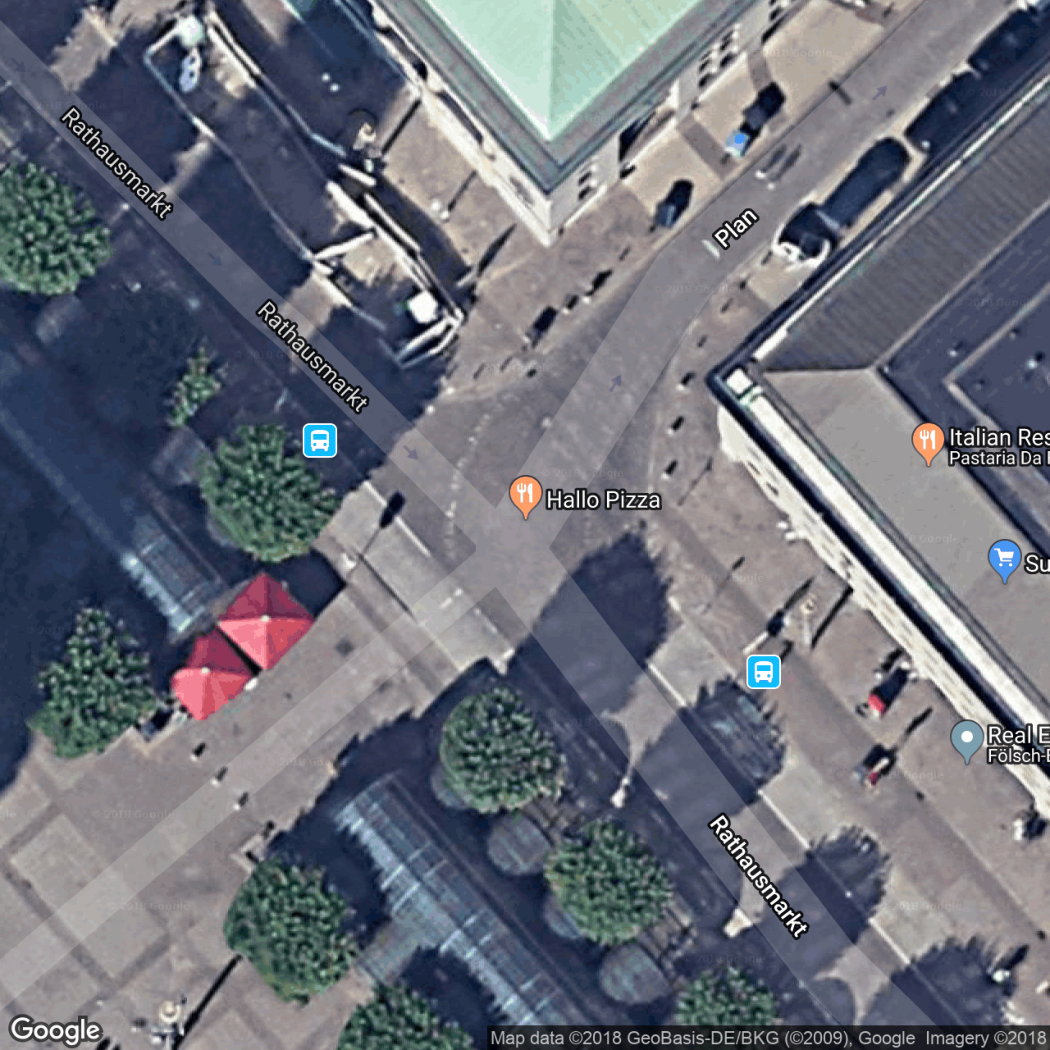
\includegraphics{figure/ham_map.pdf}

\end{frame}

\begin{frame}[fragile]{Terrain/physical maps}

\begin{itemize}
\item
  Aus Physischen Karten kann man Informationen über Berge, Flüsse und
  Seen ablesen.
\item
  Farben werden oft genutzt um Höhenunterschiede zu visualisieren
\end{itemize}

\begin{Shaded}
\begin{Highlighting}[]
\KeywordTok{qmap}\NormalTok{(}\StringTok{'Arequipa'}\NormalTok{, }\DataTypeTok{maptype=}\StringTok{"terrain"}\NormalTok{)}
\end{Highlighting}
\end{Shaded}

\end{frame}

\begin{frame}{Eine physische Karte von Arequipa}

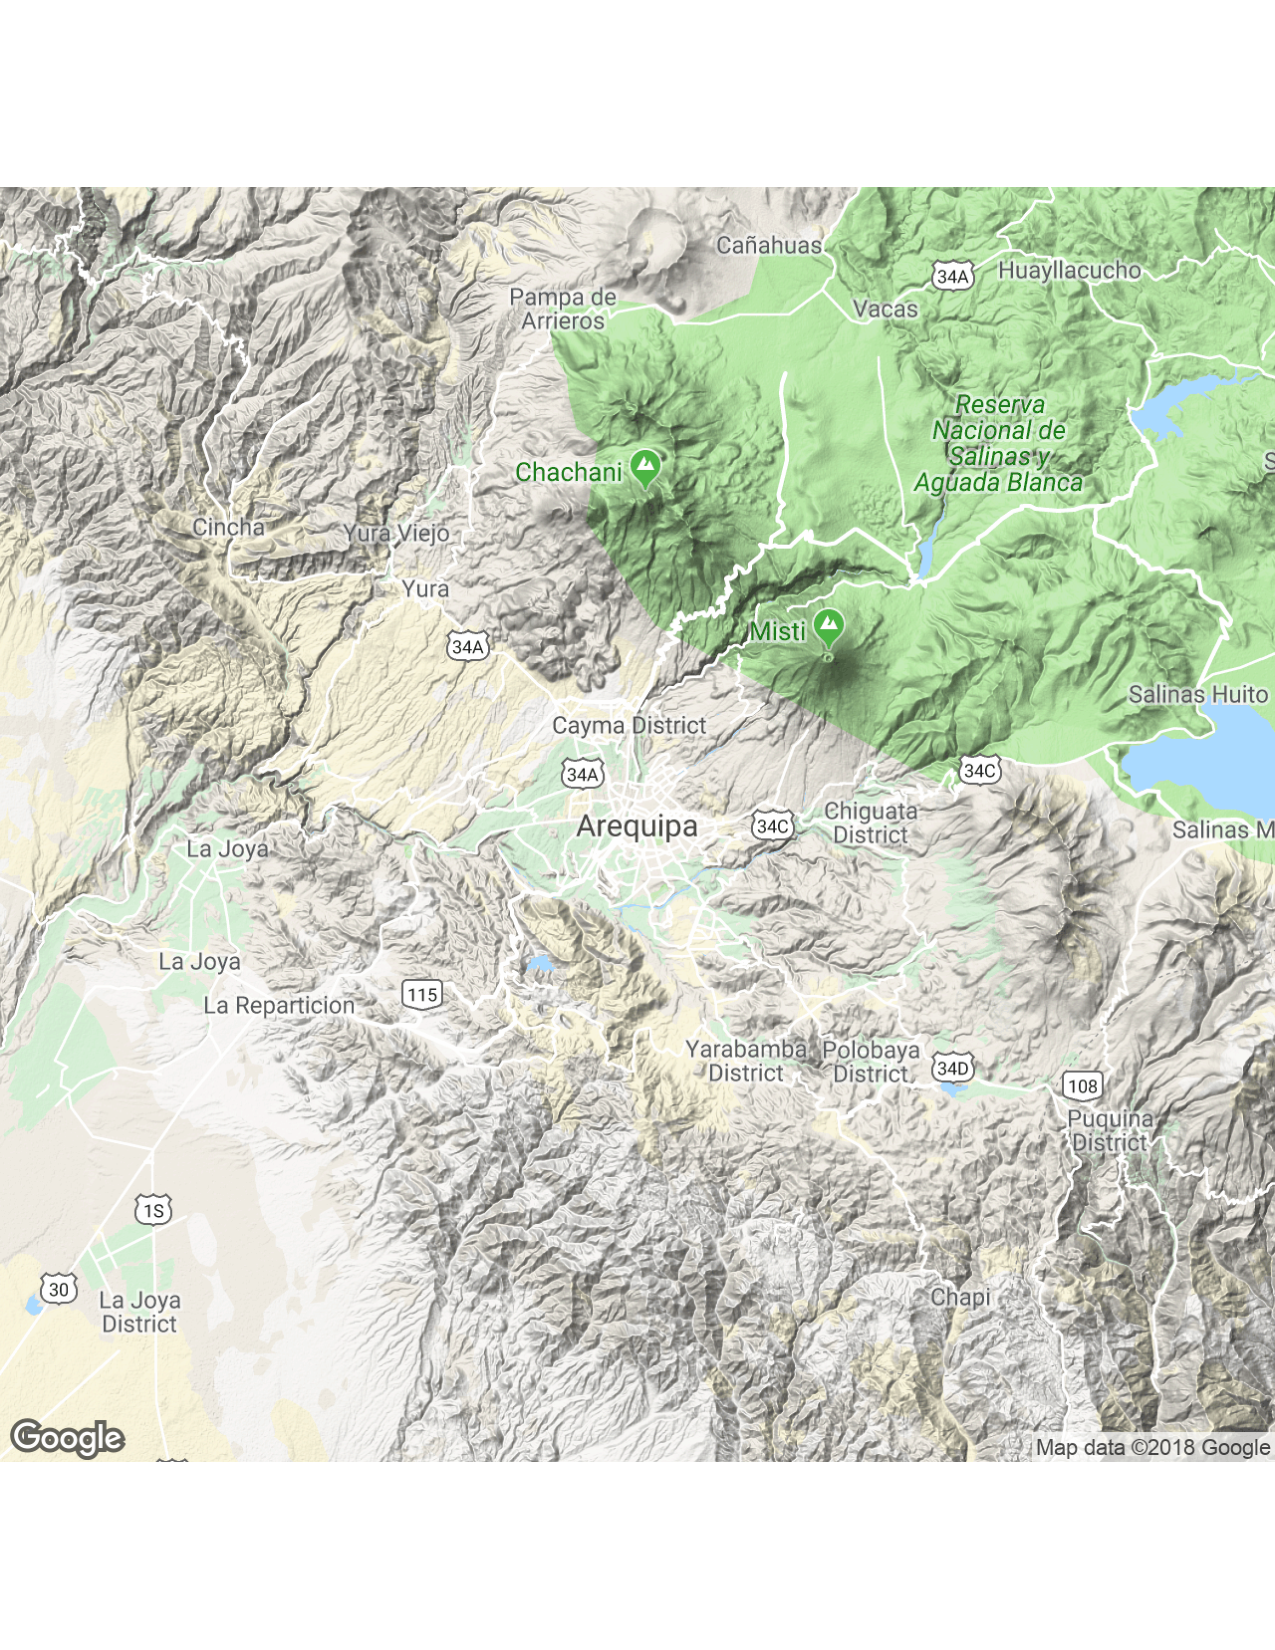
\includegraphics{figure/Areqipa.pdf}

\end{frame}

\begin{frame}{Abstrahierte Karten
(\href{http://www.designfaves.com/2014/03/abstracted-maps-reveal-cities-personalities}{http://www.designfaves.com})}

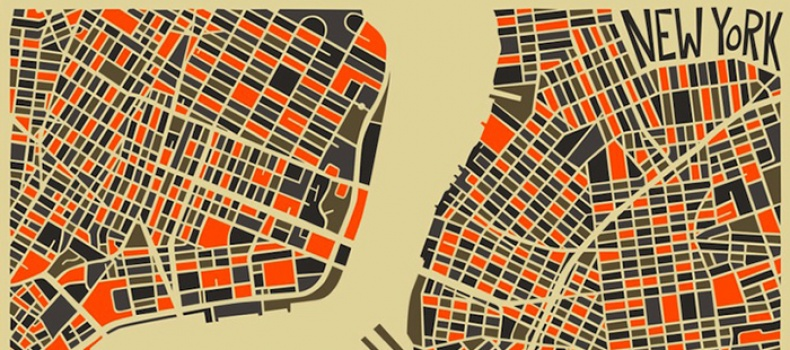
\includegraphics{figure/NYabstracted.jpg}

\begin{itemize}
\item
  Abstraktion wird genutzt um nur die essentiellen Informationen einer
  Karte zu zeigen.
\item
  Bsp. U-Bahn Karten - wichtig sind Richtungen und wenig Infos zur
  Orientierung
\item
  Im folgenden werden Karten vorgestellt, die sich gut als
  Hintergrundkarten eignen.
\end{itemize}

\end{frame}

\begin{frame}[fragile]{ggmap - maptype watercolor}

\begin{Shaded}
\begin{Highlighting}[]
\KeywordTok{qmap}\NormalTok{(}\StringTok{'Los Angeles'}\NormalTok{, }\DataTypeTok{zoom =} \DecValTok{14}\NormalTok{,}
 \DataTypeTok{maptype=}\StringTok{"watercolor"}\NormalTok{,}\DataTypeTok{source=}\StringTok{"stamen"}\NormalTok{)}
\end{Highlighting}
\end{Shaded}


\includegraphics{figure/lastamen.png}

\end{frame}

\begin{frame}{Graphiken speichern}

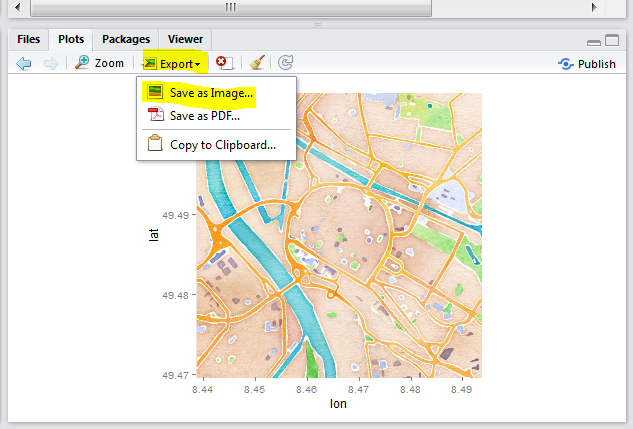
\includegraphics{figure/RstudioExport.PNG}

\end{frame}

\begin{frame}[fragile]{ggmap - ein Objekt erzeugen}

\begin{itemize}
\tightlist
\item
  \texttt{\textless{}-} ist der Zuweisungspfeil um ein Objekt zu
  erzeugen
\item
  Dieses Vorgehen macht bspw. Sinn, wenn mehrere Karten nebeneinander
  gebraucht werden.
\end{itemize}

\begin{Shaded}
\begin{Highlighting}[]
\NormalTok{MA_map <-}\StringTok{ }\KeywordTok{qmap}\NormalTok{(}\StringTok{'Mannheim'}\NormalTok{, }
               \DataTypeTok{zoom =} \DecValTok{14}\NormalTok{,}
               \DataTypeTok{maptype=}\StringTok{"toner"}\NormalTok{,}
               \DataTypeTok{source=}\StringTok{"stamen"}\NormalTok{)}
\end{Highlighting}
\end{Shaded}

\end{frame}

\begin{frame}[fragile]{\href{https://blog.dominodatalab.com/geographic-visualization-with-rs-ggmaps/}{Eine
Karte für die USA}}

\begin{itemize}
\tightlist
\item
  Mit dem Befehl \texttt{OSM\_scale\_lookup} bekommt man heraus, welchen
  Wert man für \texttt{scale} angeben muss.
\end{itemize}

\begin{Shaded}
\begin{Highlighting}[]
\KeywordTok{OSM_scale_lookup}\NormalTok{(}\DataTypeTok{zoom =} \DecValTok{10}\NormalTok{)}
\KeywordTok{qmap}\NormalTok{(}\DataTypeTok{location =} \StringTok{"Trier"}\NormalTok{, }\DataTypeTok{zoom =} \DecValTok{10}\NormalTok{, }\DataTypeTok{source =} \StringTok{"osm"}\NormalTok{,}
     \DataTypeTok{scale=}\DecValTok{575000}\NormalTok{)}
\end{Highlighting}
\end{Shaded}

\end{frame}

\begin{frame}{Cheatsheet}

\begin{itemize}
\tightlist
\item
  Cheatsheet zu
  \href{https://www.rstudio.com/wp-content/uploads/2015/04/ggplot2-cheatsheet.pdf}{data
  visualisation}
\end{itemize}

\url{https://www.rstudio.com/}

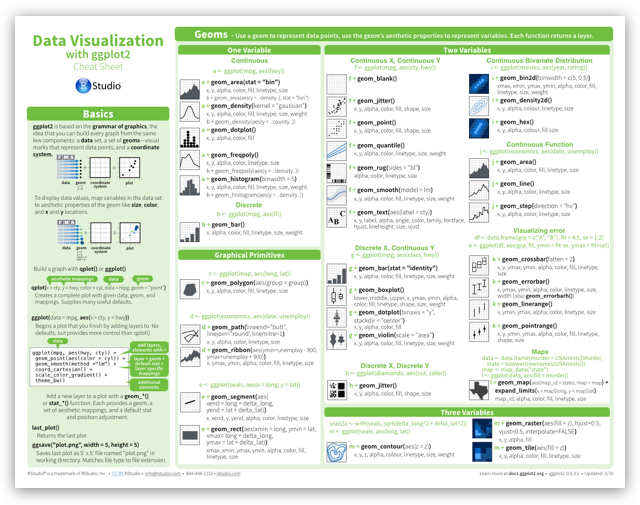
\includegraphics{figure/ggplot2-cheatsheet.png}

\end{frame}

\begin{frame}[fragile]{Resourcen und Literatur}

\begin{itemize}
\item
  Artikel von
  \href{http://journal.r-project.org/archive/2013-1/kahle-wickham.pdf}{\textbf{David
  Kahle und Hadley Wickham}} zur Nutzung von \texttt{ggmap}.
\item
  \href{http://rpackages.ianhowson.com/cran/ggmap/man/get_map.html}{\textbf{Schnell
  eine Karte bekommen}}
\item
  \href{http://www.kevjohnson.org/making-maps-in-r-part-2/}{\textbf{Karten
  machen mit R}}
\end{itemize}

\end{frame}

\begin{frame}[fragile]{Das Paket
\href{https://cran.r-project.org/web/packages/tmap/index.html}{tmap}}

\begin{itemize}
\tightlist
\item
  Mit dem Paket
  \href{http://twitter.com/sharon000/status/593028906820599808/photo/1?ref_src=twsrc\%5Etfw}{\textbf{tmap}}
  kann man thematische Karten erzeugen
\item
  Die folgenden Beispiele sind auf der
  \href{https://cran.r-project.org/web/packages/tmap/vignettes/tmap-nutshell.html}{\textbf{Vignette}}
  des Paketes basiert.
\end{itemize}

\begin{Shaded}
\begin{Highlighting}[]
\KeywordTok{install.packages}\NormalTok{(}\StringTok{"tmap"}\NormalTok{)}
\end{Highlighting}
\end{Shaded}

\begin{Shaded}
\begin{Highlighting}[]
\KeywordTok{library}\NormalTok{(tmap)}
\end{Highlighting}
\end{Shaded}

\end{frame}

\begin{frame}[fragile]{Schnelle thematische Karte}

\begin{itemize}
\item
  Mit dem Befehl
  \href{https://cran.r-project.org/web/packages/tmap/vignettes/tmap-nutshell.html}{\textbf{qtm}}
  kann man eine schnelle thematische Karte erzeugen
\item
  Beispiel aus der
  \href{https://cran.r-project.org/web/packages/tmap/vignettes/tmap-nutshell.html}{\textbf{Vignette}}
  zum Paket \texttt{tmap}
\end{itemize}

\begin{Shaded}
\begin{Highlighting}[]
\KeywordTok{data}\NormalTok{(Europe)}
\KeywordTok{qtm}\NormalTok{(Europe)}
\end{Highlighting}
\end{Shaded}

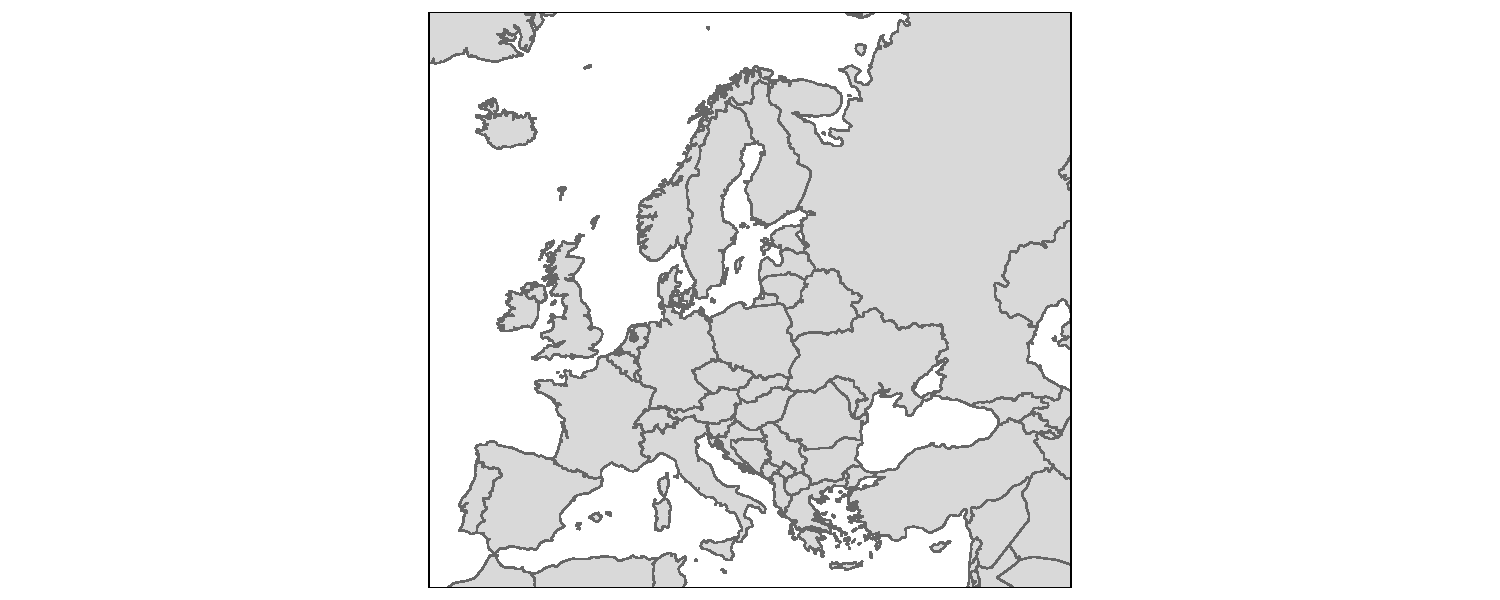
\includegraphics{slides_all2gether_part1_files/figure-beamer/unnamed-chunk-46-1.pdf}

\end{frame}

\begin{frame}{Der Europa-Datensatz}

\begin{longtable}[]{@{}lllll@{}}
\toprule
& iso\_a3 & name & sovereignt & continent\tabularnewline
\midrule
\endhead
5 & ALB & Albania & Albania & Europe\tabularnewline
6 & ALA & Aland & Finland & Europe\tabularnewline
7 & AND & Andorra & Andorra & Europe\tabularnewline
10 & ARM & Armenia & Armenia & Asia\tabularnewline
17 & AUT & Austria & Austria & Europe\tabularnewline
18 & AZE & Azerbaijan & Azerbaijan & Asia\tabularnewline
20 & BEL & Belgium & Belgium & Europe\tabularnewline
24 & BGR & Bulgaria & Bulgaria & Europe\tabularnewline
27 & BIH & Bosnia and Herz. & Bosnia and Herzegovina &
Europe\tabularnewline
29 & BLR & Belarus & Belarus & Europe\tabularnewline
\bottomrule
\end{longtable}

\end{frame}

\begin{frame}[fragile]{Um mehr Farbe in die Karte zu bekommen}

\begin{itemize}
\tightlist
\item
  Visualisierung von
  \href{http://www.naturalearthdata.com/}{\textbf{Natural Earth}} Daten
\end{itemize}

\begin{Shaded}
\begin{Highlighting}[]
\KeywordTok{qtm}\NormalTok{(Europe, }\DataTypeTok{fill=}\StringTok{"gdp_cap_est"}\NormalTok{)}
\end{Highlighting}
\end{Shaded}

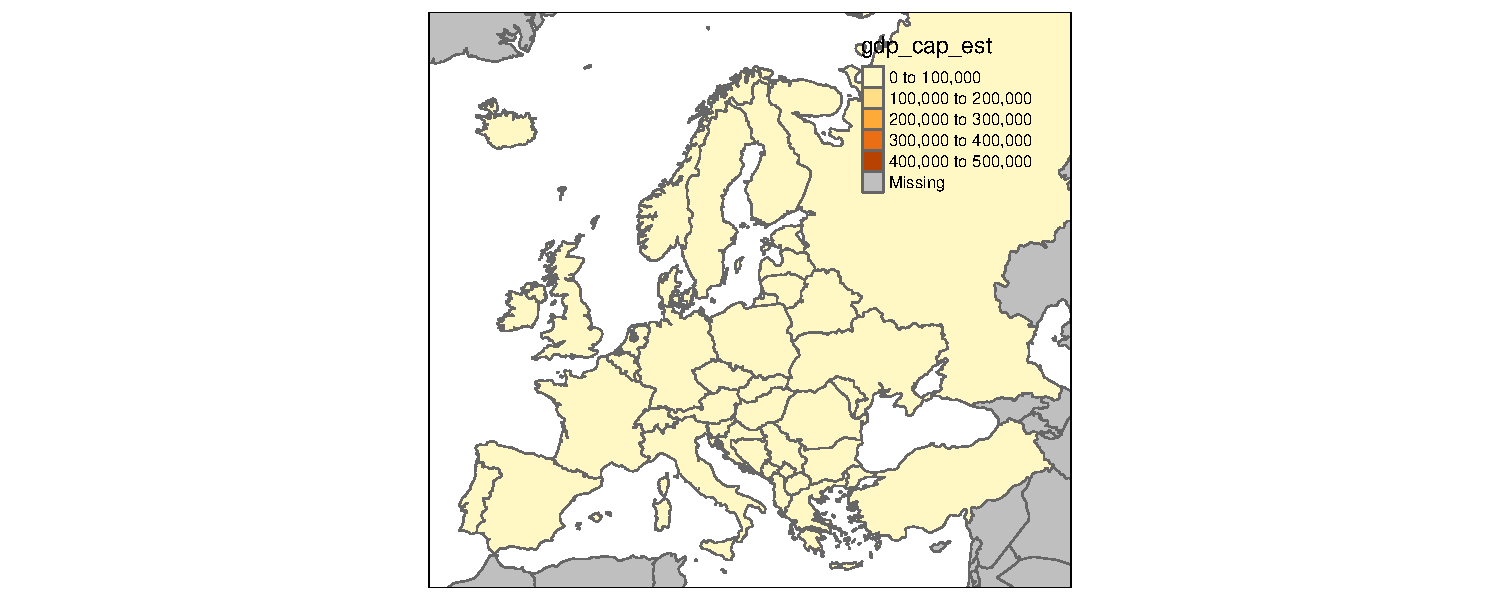
\includegraphics{slides_all2gether_part1_files/figure-beamer/unnamed-chunk-50-1.pdf}

\end{frame}

\begin{frame}[fragile]{Eine Karte mit Text}

\begin{Shaded}
\begin{Highlighting}[]
\KeywordTok{qtm}\NormalTok{(Europe, }\DataTypeTok{fill=}\StringTok{"gdp_cap_est"}\NormalTok{, }\DataTypeTok{text=}\StringTok{"iso_a3"}\NormalTok{)}
\end{Highlighting}
\end{Shaded}

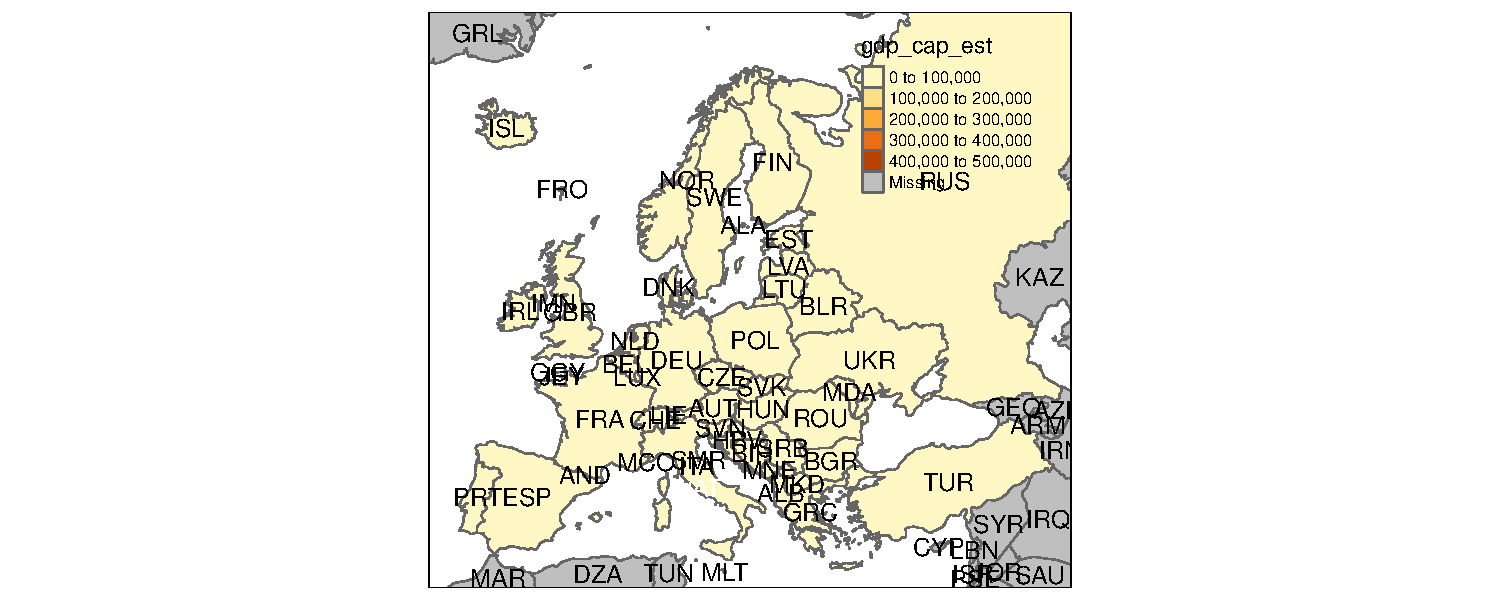
\includegraphics{slides_all2gether_part1_files/figure-beamer/unnamed-chunk-51-1.pdf}

\end{frame}

\begin{frame}[fragile]{Dieses Schema passt besser:}

\begin{block}{\href{https://en.wikipedia.org/wiki/Population_density}{\textbf{Bevölkerungsdichte}}}

\begin{Shaded}
\begin{Highlighting}[]
\KeywordTok{qtm}\NormalTok{(Europe, }\DataTypeTok{fill=}\StringTok{"gdp_cap_est"}\NormalTok{, }\DataTypeTok{text=}\StringTok{"iso_a3"}\NormalTok{, }
    \DataTypeTok{text.size=}\StringTok{"AREA"}\NormalTok{, }\DataTypeTok{root=}\DecValTok{5}\NormalTok{, }\DataTypeTok{fill.title=}\StringTok{"GDP per capita"}\NormalTok{, }
    \DataTypeTok{fill.textNA=}\StringTok{"Non-European countries"}\NormalTok{, }\DataTypeTok{theme=}\StringTok{"Europe"}\NormalTok{)}
\end{Highlighting}
\end{Shaded}

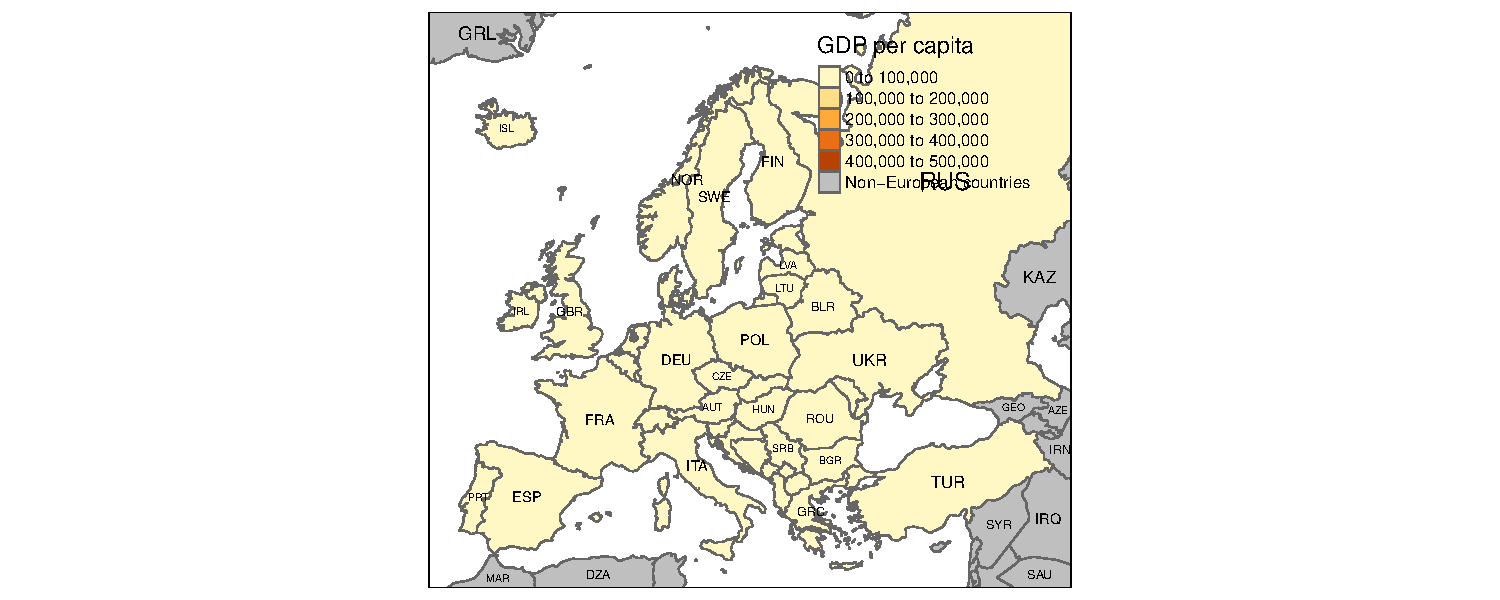
\includegraphics{slides_all2gether_part1_files/figure-beamer/unnamed-chunk-52-1.pdf}

\end{block}

\end{frame}

\begin{frame}{Themen des Europa-Datensatzes}

\begin{itemize}
\tightlist
\item
  \href{http://userpage.chemie.fu-berlin.de/diverse/doc/ISO_3166.html}{\textbf{ISO
  Klassifikation}}
\item
  Ländername
\item
  Ist das Land Teil Europas?
\item
  Fläche, Bevölkerung, Bevölkerungsdichte,
\item
  \href{https://en.wikipedia.org/wiki/Gross_domestic_product}{\textbf{Bruttoinlandsprodukt}}
\item
  Bruttoinlandsprodukt
  \href{https://en.wikipedia.org/wiki/List_of_countries_by_GDP_\%28PPP\%29_per_capita}{\textbf{zu
  Kaufkraftparitäten}}
\item
  Ökonomie, Einkommensgruppe
\end{itemize}

\end{frame}

\begin{frame}{Der Europa Datensatz - Variablen und was dahinter steckt}

\begin{longtable}[]{@{}llllll@{}}
\toprule
& iso\_a3 & name & sovereignt & continent & part\tabularnewline
\midrule
\endhead
5 & ALB & Albania & Albania & Europe & Southern Europe\tabularnewline
6 & ALA & Aland & Finland & Europe & Northern Europe\tabularnewline
7 & AND & Andorra & Andorra & Europe & Southern Europe\tabularnewline
10 & ARM & Armenia & Armenia & Asia & NA\tabularnewline
17 & AUT & Austria & Austria & Europe & Western Europe\tabularnewline
18 & AZE & Azerbaijan & Azerbaijan & Asia & NA\tabularnewline
20 & BEL & Belgium & Belgium & Europe & Western Europe\tabularnewline
24 & BGR & Bulgaria & Bulgaria & Europe & Eastern Europe\tabularnewline
\bottomrule
\end{longtable}

\end{frame}

\begin{frame}[fragile]{Die Variable \texttt{continent}}

\begin{Shaded}
\begin{Highlighting}[]
\KeywordTok{qtm}\NormalTok{(Europe, }\DataTypeTok{fill=}\StringTok{"continent"}\NormalTok{)}
\end{Highlighting}
\end{Shaded}

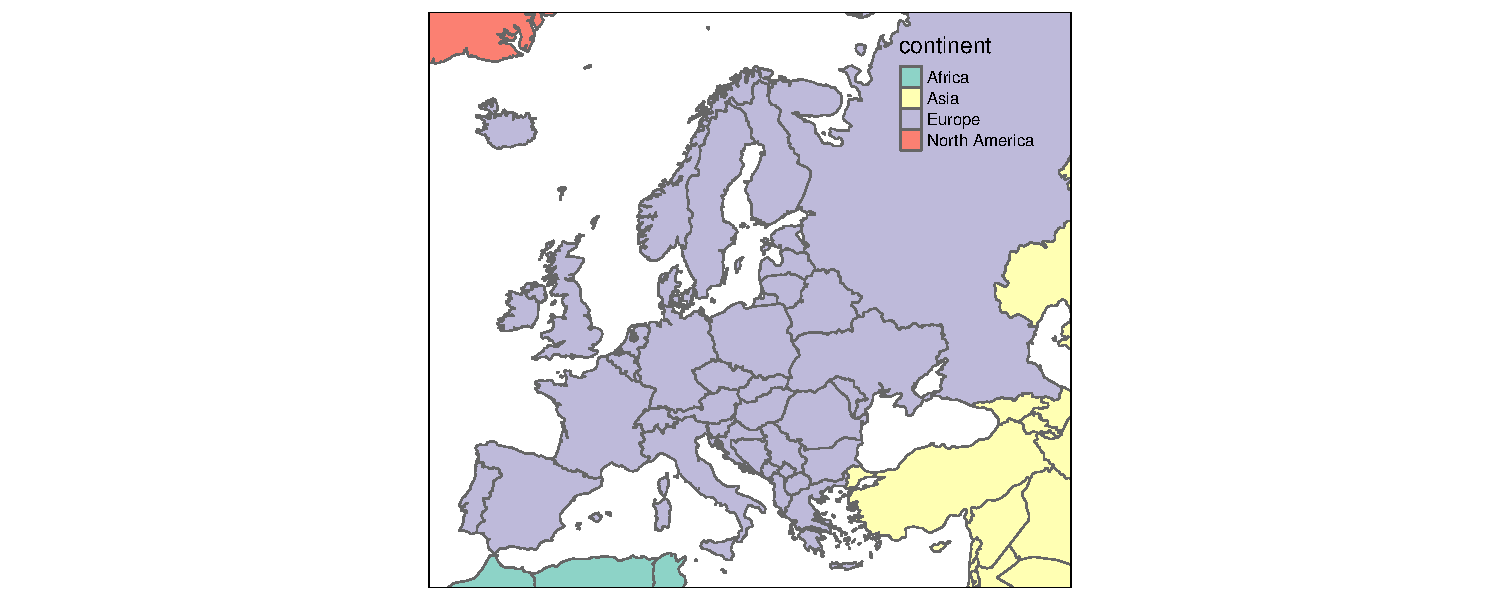
\includegraphics{slides_all2gether_part1_files/figure-beamer/unnamed-chunk-56-1.pdf}

\end{frame}

\begin{frame}[fragile]{Die Variable \texttt{part}}

\begin{Shaded}
\begin{Highlighting}[]
\KeywordTok{qtm}\NormalTok{(Europe, }\DataTypeTok{fill=}\StringTok{"part"}\NormalTok{,}\DataTypeTok{fill.title=}\StringTok{"Teil von Europa"}\NormalTok{)}
\end{Highlighting}
\end{Shaded}

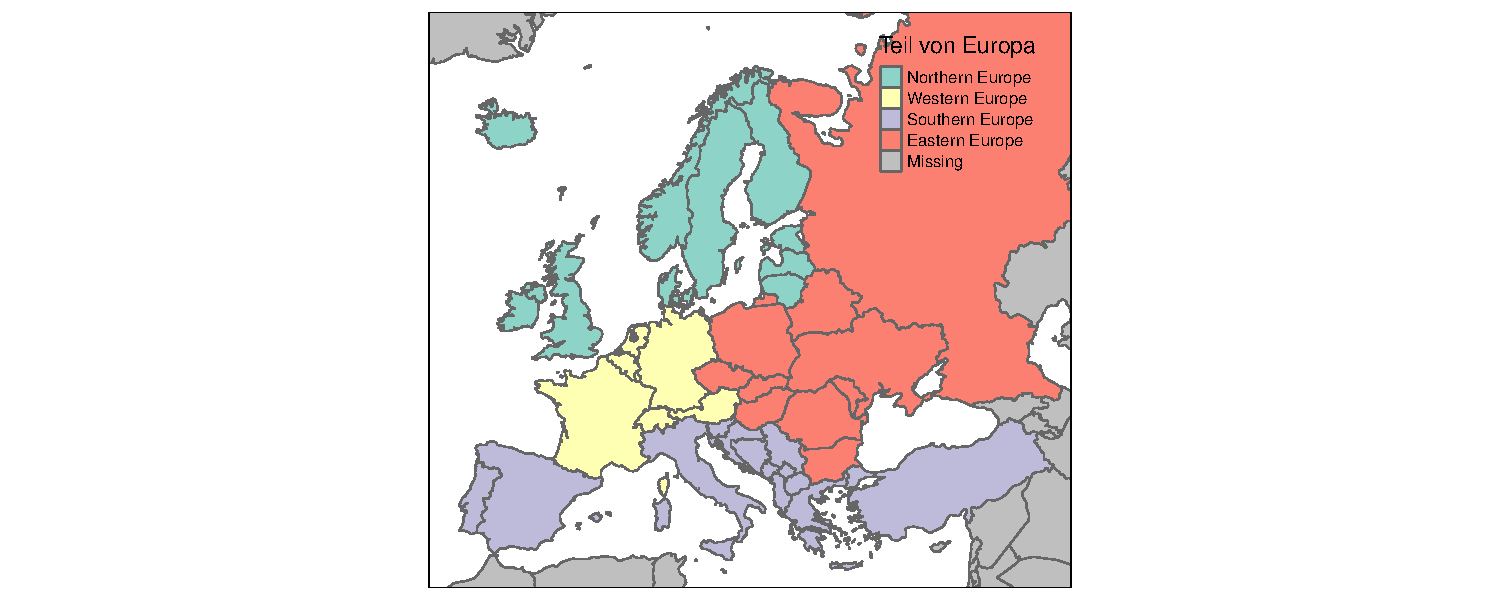
\includegraphics{slides_all2gether_part1_files/figure-beamer/unnamed-chunk-57-1.pdf}

\end{frame}

\begin{frame}[fragile]{Die Variable \texttt{area}}

\begin{Shaded}
\begin{Highlighting}[]
\KeywordTok{qtm}\NormalTok{(Europe, }\DataTypeTok{fill=}\StringTok{"area"}\NormalTok{) }\CommentTok{# Russia is huge}
\end{Highlighting}
\end{Shaded}

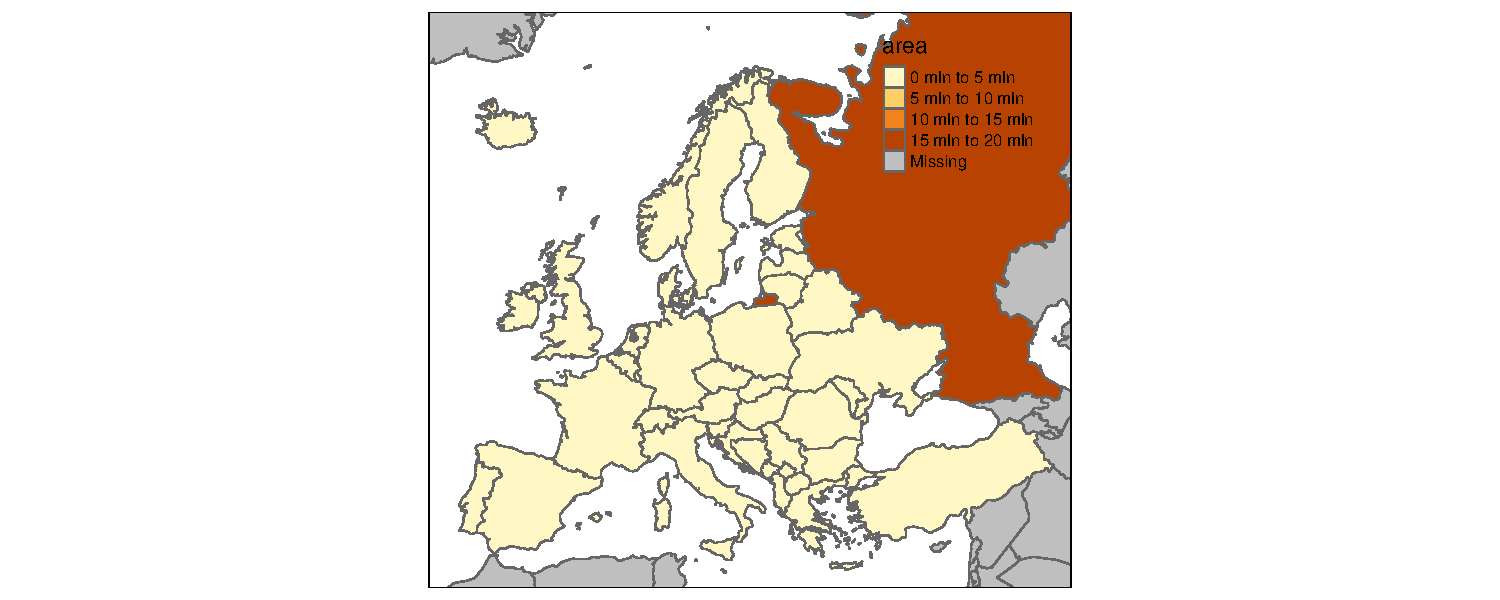
\includegraphics{slides_all2gether_part1_files/figure-beamer/unnamed-chunk-58-1.pdf}

\end{frame}

\begin{frame}[fragile]{Bevölkerung}

\begin{Shaded}
\begin{Highlighting}[]
\KeywordTok{qtm}\NormalTok{(Europe, }\DataTypeTok{fill=}\StringTok{"pop_est"}\NormalTok{,}\DataTypeTok{fill.title=}\StringTok{"Population"}\NormalTok{) }
\end{Highlighting}
\end{Shaded}

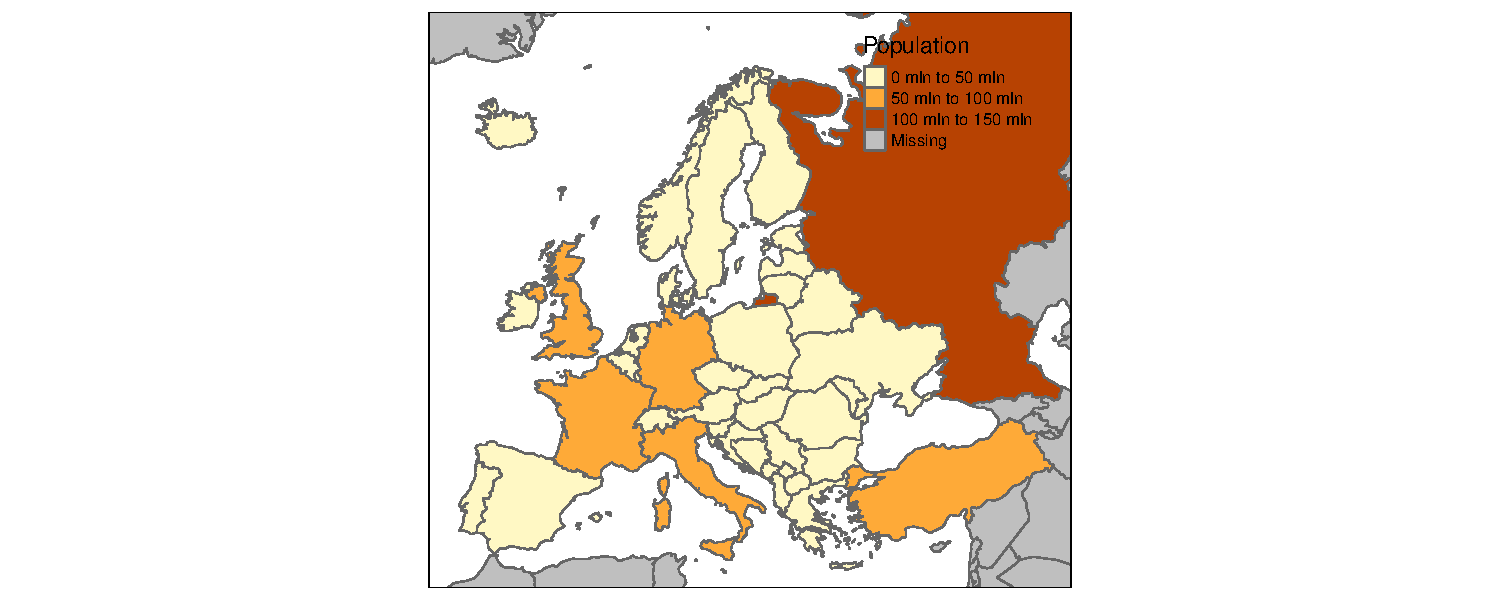
\includegraphics{slides_all2gether_part1_files/figure-beamer/unnamed-chunk-59-1.pdf}

\end{frame}

\begin{frame}[fragile]{Ökonomie}

\begin{Shaded}
\begin{Highlighting}[]
\KeywordTok{qtm}\NormalTok{(Europe, }\DataTypeTok{fill=}\StringTok{"economy"}\NormalTok{) }
\end{Highlighting}
\end{Shaded}

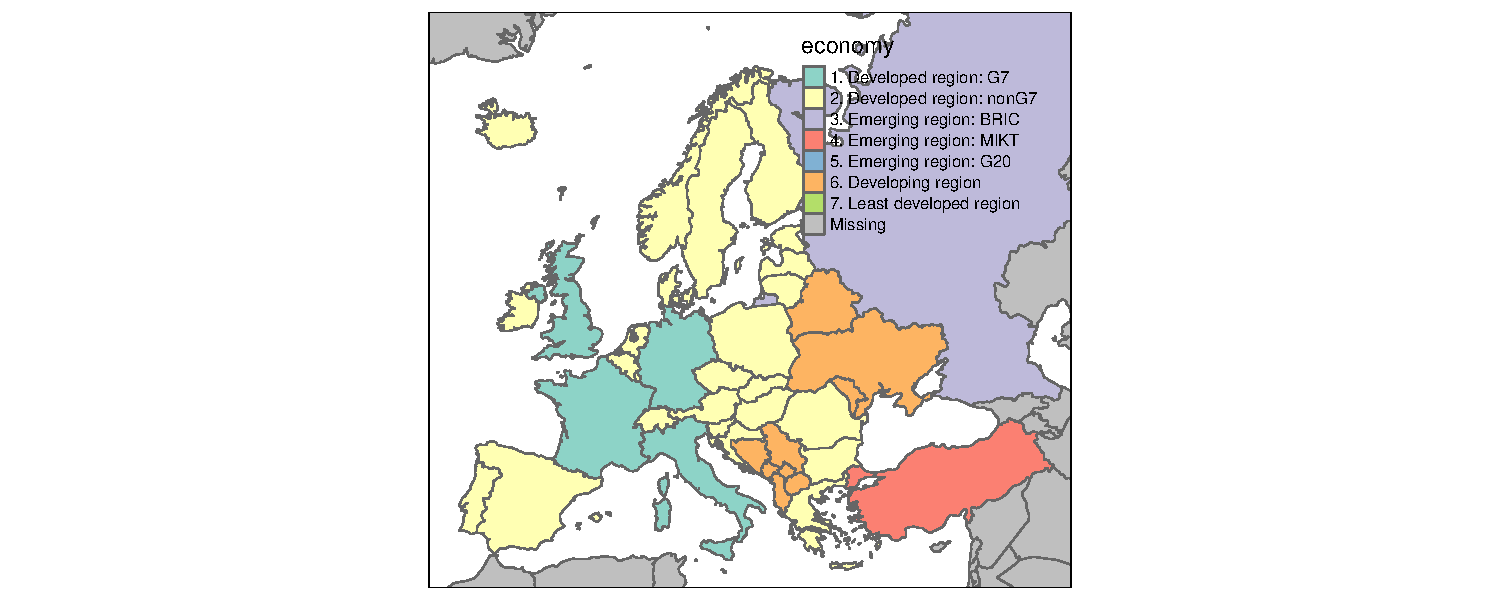
\includegraphics{slides_all2gether_part1_files/figure-beamer/unnamed-chunk-61-1.pdf}

\end{frame}

\begin{frame}[fragile]{Einkommensgruppe}

\begin{Shaded}
\begin{Highlighting}[]
\KeywordTok{qtm}\NormalTok{(Europe, }\DataTypeTok{fill=}\StringTok{"income_grp"}\NormalTok{,}\DataTypeTok{fill.title=}\StringTok{"Income group"}\NormalTok{) }
\end{Highlighting}
\end{Shaded}

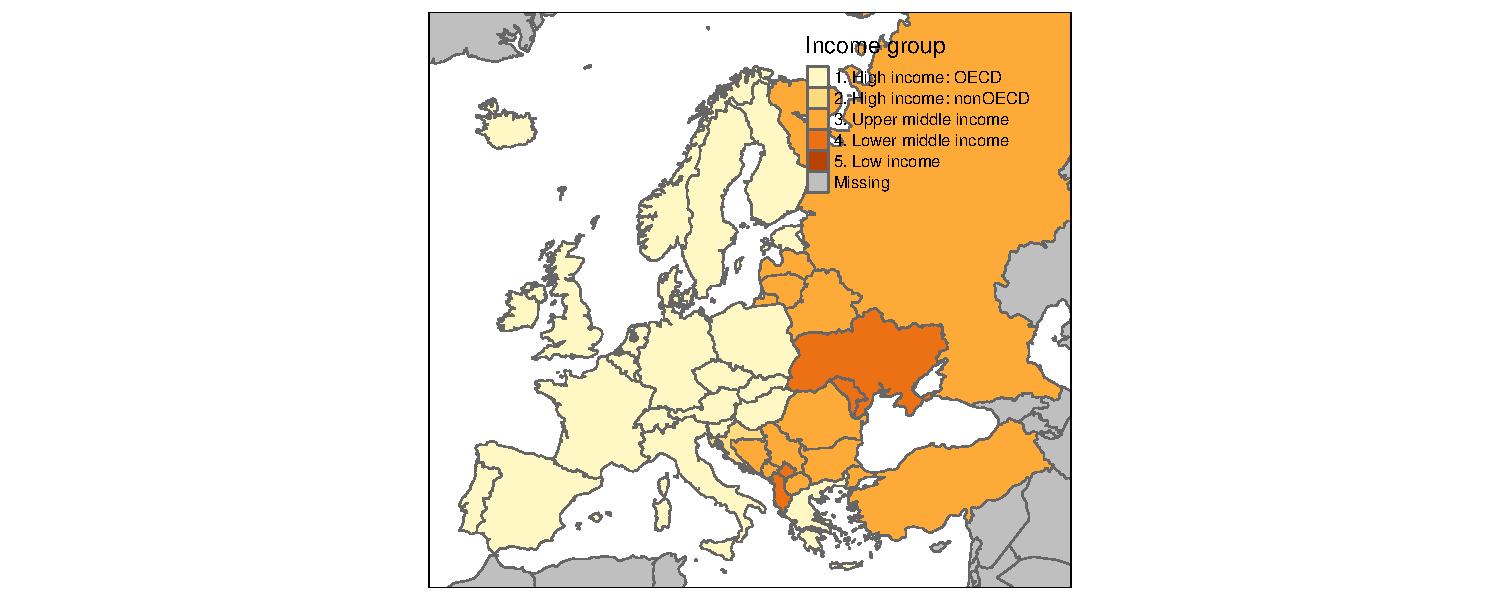
\includegraphics{slides_all2gether_part1_files/figure-beamer/unnamed-chunk-62-1.pdf}

\end{frame}

\begin{frame}{Der Welt-Datensatz im Paket \texttt{tmap}}

\begin{longtable}[]{@{}llllllrrrrrllrrr@{}}
\toprule
& iso\_a3 & name & sovereignt & continent & subregion & area & pop\_est
& pop\_est\_dens & gdp\_md\_est & gdp\_cap\_est & economy & income\_grp
& life\_exp & well\_being & HPI\tabularnewline
\midrule
\endhead
2 & AFG & Afghanistan & Afghanistan & Asia & Southern Asia & 652860.000
& 28400000 & 43.5009037 & 22270 & 784.1549 & 7. Least developed region &
5. Low income & 48.7 & 4.758381 & 36.75366\tabularnewline
3 & AGO & Angola & Angola & Africa & Middle Africa & 1246700.000 &
12799293 & 10.2665381 & 110300 & 8617.6635 & 7. Least developed region &
3. Upper middle income & 51.1 & 4.206092 & 33.20143\tabularnewline
5 & ALB & Albania & Albania & Europe & Southern Europe & 27400.000 &
3639453 & 132.8267518 & 21810 & 5992.6588 & 6. Developing region & 4.
Lower middle income & 76.9 & 5.268937 & 54.05118\tabularnewline
8 & ARE & United Arab Emirates & United Arab Emirates & Asia & Western
Asia & 83600.000 & 4798491 & 57.3982177 & 184300 & 38407.9078 & 6.
Developing region & 2. High income: nonOECD & 76.5 & 7.196803 &
31.77827\tabularnewline
9 & ARG & Argentina & Argentina & South America & South America &
2736690.000 & 40913584 & 14.9500250 & 573900 & 14027.1261 & 5. Emerging
region: G20 & 3. Upper middle income & 75.9 & 6.441067 &
54.05504\tabularnewline
10 & ARM & Armenia & Armenia & Asia & Western Asia & 28470.000 & 2967004
& 104.2151036 & 18770 & 6326.2469 & 6. Developing region & 4. Lower
middle income & 74.2 & 4.367811 & 46.00319\tabularnewline
12 & ATA & Antarctica & Antarctica & Antarctica & Antarctica &
10866664.407 & 3802 & 0.0003499 & NA & NA & 6. Developing region & 2.
High income: nonOECD & NA & NA & NA\tabularnewline
14 & ATF & Fr. S. Antarctic Lands & France & Seven seas (open ocean) &
Seven seas (open ocean) & 6187.205 & 140 & 0.0226273 & 16 & 114285.7143
& 6. Developing region & 2. High income: nonOECD & NA & NA &
NA\tabularnewline
16 & AUS & Australia & Australia & Oceania & Australia and New Zealand &
7682300.000 & 21262641 & 2.7677442 & 800200 & 37634.0832 & 2. Developed
region: nonG7 & 1. High income: OECD & 81.9 & 7.405616 &
41.97981\tabularnewline
17 & AUT & Austria & Austria & Europe & Western Europe & 82409.000 &
8210281 & 99.6284508 & 329500 & 40132.6093 & 2. Developed region: nonG7
& 1. High income: OECD & 80.9 & 7.346036 & 47.08514\tabularnewline
18 & AZE & Azerbaijan & Azerbaijan & Asia & Western Asia & 82658.000 &
8238672 & 99.6718043 & 77610 & 9420.2075 & 6. Developing region & 3.
Upper middle income & 70.7 & 4.218611 & 40.88457\tabularnewline
19 & BDI & Burundi & Burundi & Africa & Eastern Africa & 25680.000 &
8988091 & 350.0035436 & 3102 & 345.1233 & 7. Least developed region & 5.
Low income & 50.4 & 3.791681 & 30.51501\tabularnewline
20 & BEL & Belgium & Belgium & Europe & Western Europe & 30280.000 &
10414336 & 343.9344782 & 389300 & 37381.1638 & 2. Developed region:
nonG7 & 1. High income: OECD & 80.0 & 6.853514 & 37.09053\tabularnewline
21 & BEN & Benin & Benin & Africa & Western Africa & 112760.000 &
8791832 & 77.9694218 & 12830 & 1459.3090 & 7. Least developed region &
5. Low income & 56.1 & 3.667140 & 31.08321\tabularnewline
22 & BFA & Burkina Faso & Burkina Faso & Africa & Western Africa &
273600.000 & 15746232 & 57.5520175 & 17820 & 1131.6993 & 7. Least
developed region & 5. Low income & 55.4 & 4.035560 &
31.79385\tabularnewline
\bottomrule
\end{longtable}

\end{frame}

\begin{frame}[fragile]{Welt - Länder nach Einkommensgruppe}

\begin{Shaded}
\begin{Highlighting}[]
\KeywordTok{qtm}\NormalTok{(World, }\DataTypeTok{fill=}\StringTok{"income_grp"}\NormalTok{,}\DataTypeTok{fill.title=}\StringTok{"Income group"}\NormalTok{) }
\end{Highlighting}
\end{Shaded}

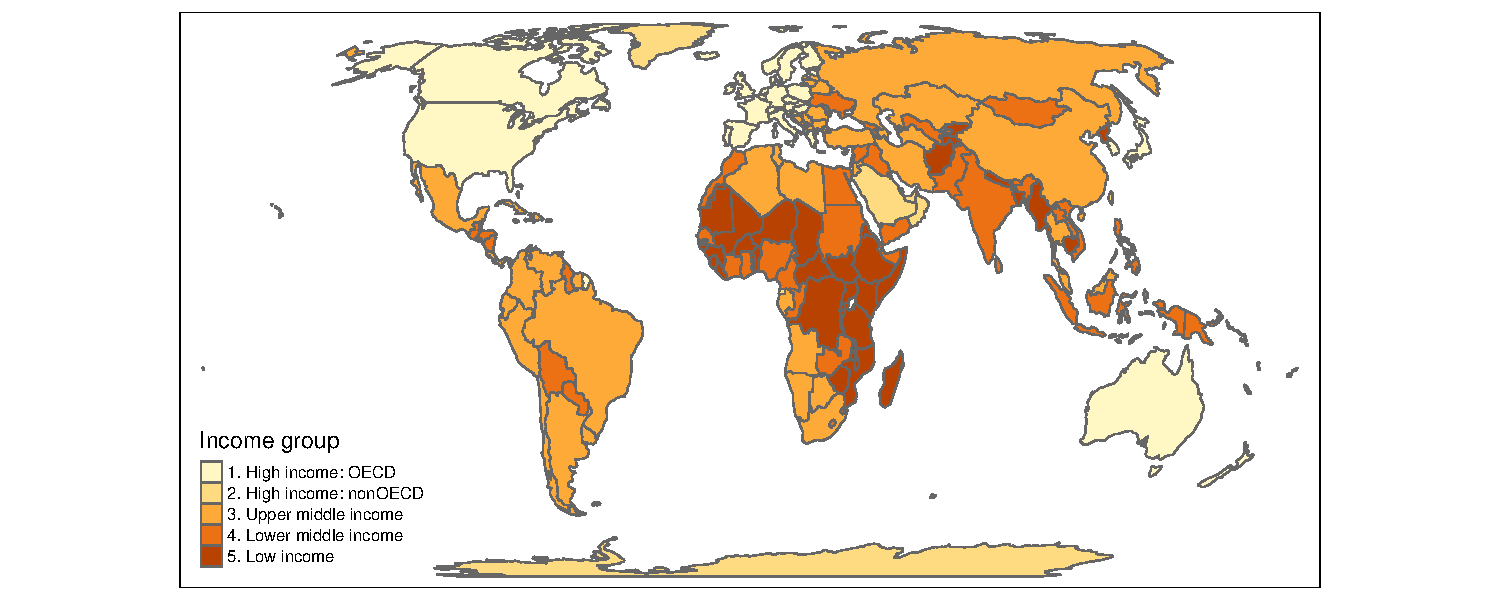
\includegraphics{slides_all2gether_part1_files/figure-beamer/unnamed-chunk-65-1.pdf}

\end{frame}

\begin{frame}{Ein Datensatz zu den Provinzen in den Niederlanden
(R-Paket \texttt{tmap})}

\begin{longtable}[]{@{}lllrrrrrrrrrrr@{}}
\toprule
& code & name & population & pop\_men & pop\_women & pop\_0\_14 &
pop\_15\_24 & pop\_25\_44 & pop\_45\_64 & pop\_65plus & origin\_native &
origin\_west & origin\_non\_west\tabularnewline
\midrule
\endhead
0 & 20 & Groningen & 582705 & 289795 & 292875 & 15 & 15 & 25 & 27 & 18 &
87 & 7 & 6\tabularnewline
1 & 21 & Friesland & 646290 & 323215 & 323055 & 17 & 12 & 24 & 28 & 19 &
91 & 5 & 4\tabularnewline
2 & 22 & Drenthe & 488970 & 242225 & 246755 & 17 & 10 & 22 & 30 & 21 &
91 & 6 & 3\tabularnewline
3 & 23 & Overijssel & 1139680 & 570185 & 569465 & 18 & 12 & 25 & 27 & 18
& 86 & 7 & 7\tabularnewline
4 & 24 & Flevoland & 399885 & 199940 & 199940 & 20 & 13 & 27 & 28 & 12 &
71 & 9 & 20\tabularnewline
5 & 25 & Gelderland & 2019635 & 997805 & 1021790 & 17 & 12 & 24 & 29 &
18 & 85 & 8 & 7\tabularnewline
\bottomrule
\end{longtable}

\end{frame}

\begin{frame}[fragile]{Niederlande - Bevölkerung in den Provinzen}

\begin{Shaded}
\begin{Highlighting}[]
\KeywordTok{qtm}\NormalTok{(NLD_prov, }\DataTypeTok{fill=}\StringTok{"population"}\NormalTok{,}\DataTypeTok{fill.title=}\StringTok{"population"}\NormalTok{) }
\end{Highlighting}
\end{Shaded}

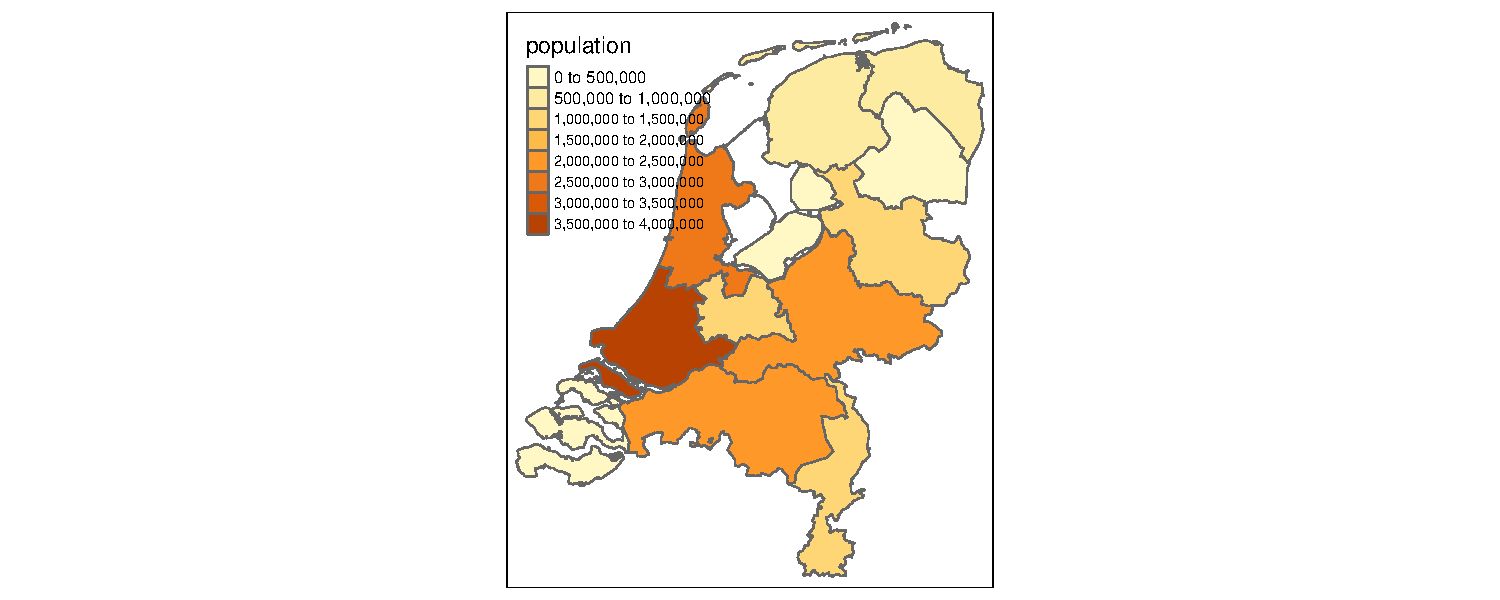
\includegraphics{slides_all2gether_part1_files/figure-beamer/unnamed-chunk-68-1.pdf}

\end{frame}

\begin{frame}[fragile]{Anteile berechnen}

\begin{Shaded}
\begin{Highlighting}[]
\NormalTok{pop <-}\StringTok{ }\NormalTok{NLD_prov}\OperatorTok{@}\NormalTok{data}\OperatorTok{$}\NormalTok{population}
\NormalTok{pop}
\end{Highlighting}
\end{Shaded}

\begin{verbatim}
##  [1]  582705  646290  488970 1139680  399885 2019635 1253645 2741320
##  [9] 3576960  380610 2479220 1119980
\end{verbatim}

\begin{Shaded}
\begin{Highlighting}[]
\NormalTok{popmen <-}\StringTok{ }\NormalTok{NLD_prov}\OperatorTok{@}\NormalTok{data}\OperatorTok{$}\NormalTok{pop_men}
\NormalTok{popmen}
\end{Highlighting}
\end{Shaded}

\begin{verbatim}
##  [1]  289795  323215  242225  570185  199940  997805  613645 1349610
##  [9] 1764855  188655 1238600  555450
\end{verbatim}

\begin{Shaded}
\begin{Highlighting}[]
\NormalTok{prop <-}\StringTok{ }\NormalTok{popmen}\OperatorTok{/}\NormalTok{pop}
\NormalTok{prop}
\end{Highlighting}
\end{Shaded}

\begin{verbatim}
##  [1] 0.4973271 0.5001083 0.4953780 0.5003027 0.4999937 0.4940521 0.4894887
##  [8] 0.4923212 0.4933952 0.4956649 0.4995926 0.4959464
\end{verbatim}

\end{frame}

\begin{frame}[fragile]{Exkurs: Barplot vom Männeranteil}

\begin{Shaded}
\begin{Highlighting}[]
\KeywordTok{barplot}\NormalTok{(prop)}
\end{Highlighting}
\end{Shaded}

\begin{block}{Barplot mit Farbe}

\begin{Shaded}
\begin{Highlighting}[]
\KeywordTok{barplot}\NormalTok{(prop,}\DataTypeTok{col=}\StringTok{"blue"}\NormalTok{)}
\end{Highlighting}
\end{Shaded}

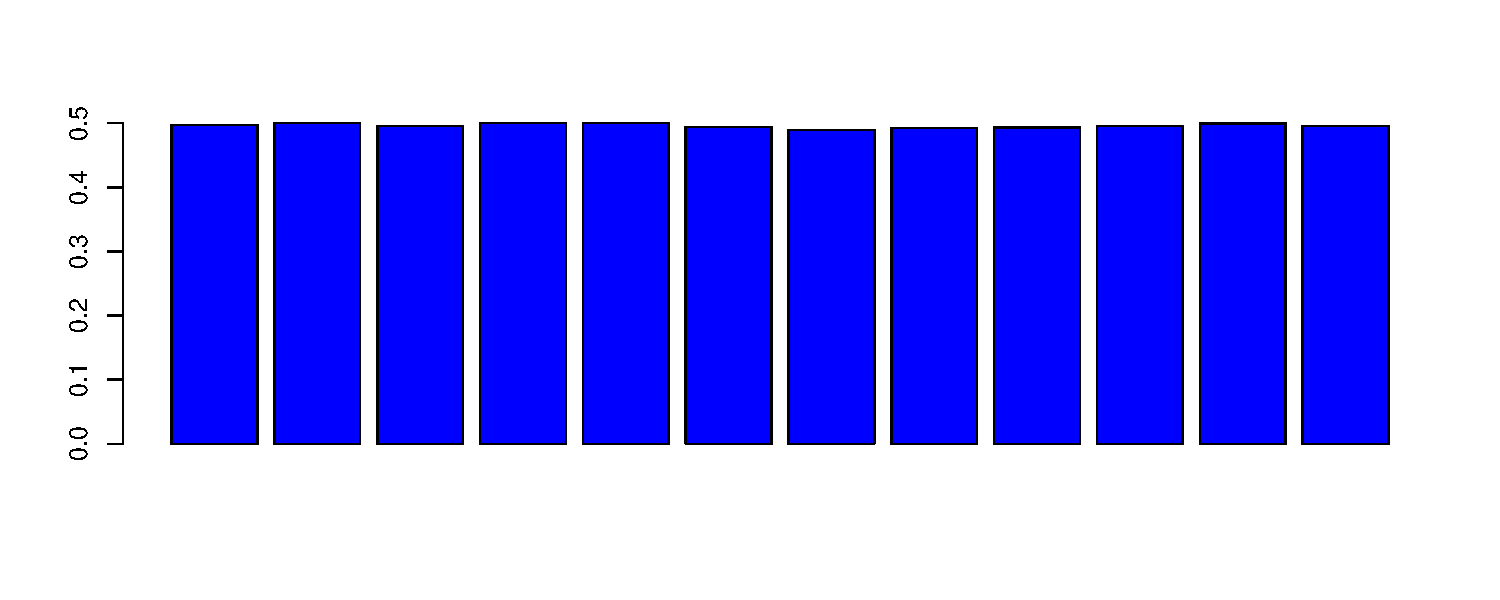
\includegraphics{slides_all2gether_part1_files/figure-beamer/unnamed-chunk-73-1.pdf}

\end{block}

\end{frame}

\begin{frame}[fragile]{Niederlnade - Anteil Männer}

Information in Datensatz einspeisen

\begin{Shaded}
\begin{Highlighting}[]
\NormalTok{NLD_prov}\OperatorTok{@}\NormalTok{data}\OperatorTok{$}\NormalTok{proportion <-}\StringTok{ }\NormalTok{prop}
\end{Highlighting}
\end{Shaded}

\begin{Shaded}
\begin{Highlighting}[]
\KeywordTok{qtm}\NormalTok{(NLD_prov, }\DataTypeTok{fill=}\StringTok{"proportion"}\NormalTok{,}\DataTypeTok{fill.title=}\StringTok{"proportion"}\NormalTok{) }
\end{Highlighting}
\end{Shaded}

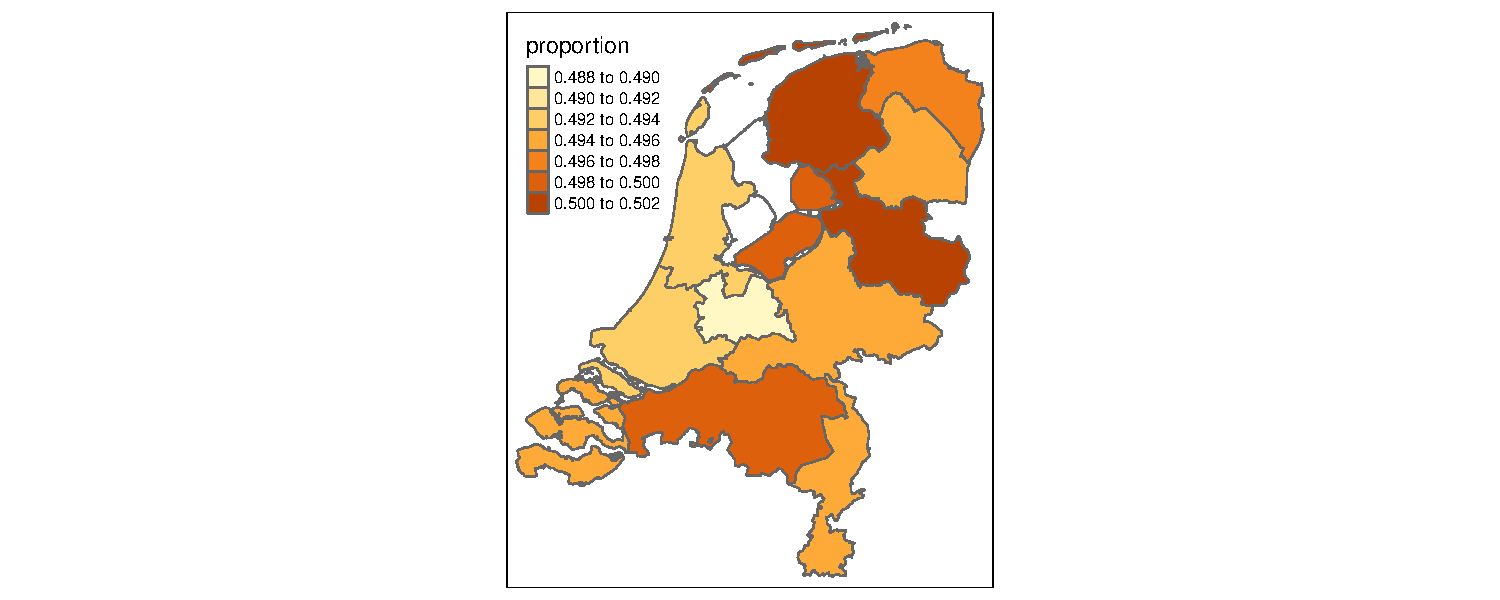
\includegraphics{slides_all2gether_part1_files/figure-beamer/unnamed-chunk-75-1.pdf}

\end{frame}

\begin{frame}[fragile]{Ein Datensatz zu den Gemeinden in den
Niederlanden}

\begin{Shaded}
\begin{Highlighting}[]
\KeywordTok{data}\NormalTok{(NLD_muni)}
\end{Highlighting}
\end{Shaded}

\begin{longtable}[]{@{}lllr@{}}
\toprule
& name & province & population\tabularnewline
\midrule
\endhead
0 & Appingedam & Groningen & 12065\tabularnewline
1 & Bedum & Groningen & 10495\tabularnewline
2 & Bellingwedde & Groningen & 8920\tabularnewline
3 & Ten Boer & Groningen & 7480\tabularnewline
4 & Delfzijl & Groningen & 25695\tabularnewline
5 & Groningen & Groningen & 198315\tabularnewline
6 & Grootegast & Groningen & 12165\tabularnewline
7 & Haren & Groningen & 18780\tabularnewline
8 & Hoogezand-Sappemeer & Groningen & 34305\tabularnewline
9 & Leek & Groningen & 19595\tabularnewline
10 & Loppersum & Groningen & 10195\tabularnewline
11 & Marum & Groningen & 10375\tabularnewline
12 & Almere & Flevoland & 196010\tabularnewline
13 & Stadskanaal & Groningen & 32800\tabularnewline
14 & Slochteren & Groningen & 15545\tabularnewline
15 & Veendam & Groningen & 27790\tabularnewline
16 & Vlagtwedde & Groningen & 15905\tabularnewline
17 & Zeewolde & Flevoland & 21500\tabularnewline
18 & Winsum & Groningen & 13850\tabularnewline
19 & Zuidhorn & Groningen & 18775\tabularnewline
20 & Dongeradeel & Friesland & 24160\tabularnewline
21 & Achtkarspelen & Friesland & 28015\tabularnewline
22 & Ameland & Friesland & 3575\tabularnewline
23 & het Bildt & Friesland & 10625\tabularnewline
24 & Franekeradeel & Friesland & 20445\tabularnewline
25 & Harlingen & Friesland & 15820\tabularnewline
26 & Heerenveen & Friesland & 49900\tabularnewline
27 & Kollumerland en Nieuwkruisland & Friesland & 12875\tabularnewline
28 & Leeuwarden & Friesland & 107340\tabularnewline
29 & Leeuwarderadeel & Friesland & 10275\tabularnewline
30 & Ooststellingwerf & Friesland & 25670\tabularnewline
31 & Opsterland & Friesland & 29860\tabularnewline
32 & Schiermonnikoog & Friesland & 940\tabularnewline
33 & Smallingerland & Friesland & 55465\tabularnewline
34 & Terschelling & Friesland & 4780\tabularnewline
35 & Vlieland & Friesland & 1110\tabularnewline
36 & Weststellingwerf & Friesland & 25455\tabularnewline
37 & Assen & Drenthe & 67190\tabularnewline
38 & Coevorden & Drenthe & 35770\tabularnewline
39 & Emmen & Drenthe & 108050\tabularnewline
40 & Hoogeveen & Drenthe & 54665\tabularnewline
41 & Meppel & Drenthe & 32865\tabularnewline
42 & Littenseradiel & Friesland & 10925\tabularnewline
43 & Almelo & Overijssel & 72460\tabularnewline
44 & Borne & Overijssel & 21885\tabularnewline
45 & Dalfsen & Overijssel & 27675\tabularnewline
46 & Deventer & Overijssel & 98320\tabularnewline
47 & Enschede & Overijssel & 158585\tabularnewline
48 & Haaksbergen & Overijssel & 24345\tabularnewline
49 & Hardenberg & Overijssel & 59575\tabularnewline
50 & Hellendoorn & Overijssel & 35710\tabularnewline
51 & Hengelo & Overijssel & 80955\tabularnewline
52 & Kampen & Overijssel & 51090\tabularnewline
53 & Losser & Overijssel & 22610\tabularnewline
54 & Noordoostpolder & Flevoland & 46355\tabularnewline
55 & Oldenzaal & Overijssel & 32135\tabularnewline
56 & Ommen & Overijssel & 17360\tabularnewline
57 & Raalte & Overijssel & 36520\tabularnewline
58 & Staphorst & Overijssel & 16365\tabularnewline
59 & Tubbergen & Overijssel & 21205\tabularnewline
60 & Urk & Flevoland & 19470\tabularnewline
61 & Wierden & Overijssel & 23910\tabularnewline
62 & Zwolle & Overijssel & 123160\tabularnewline
63 & Rijnwaarden & Gelderland & 10915\tabularnewline
64 & Aalten & Gelderland & 27010\tabularnewline
65 & Apeldoorn & Gelderland & 157545\tabularnewline
66 & Arnhem & Gelderland & 150820\tabularnewline
67 & Barneveld & Gelderland & 54150\tabularnewline
68 & Beuningen & Gelderland & 25285\tabularnewline
69 & Brummen & Gelderland & 21175\tabularnewline
70 & Buren & Gelderland & 26020\tabularnewline
71 & Culemborg & Gelderland & 27590\tabularnewline
72 & Doesburg & Gelderland & 11435\tabularnewline
73 & Doetinchem & Gelderland & 56345\tabularnewline
74 & Druten & Gelderland & 18210\tabularnewline
75 & Duiven & Gelderland & 25610\tabularnewline
76 & Ede & Gelderland & 110655\tabularnewline
77 & Elburg & Gelderland & 22645\tabularnewline
78 & Epe & Gelderland & 32350\tabularnewline
79 & Ermelo & Gelderland & 26045\tabularnewline
80 & Geldermalsen & Gelderland & 26300\tabularnewline
81 & Groesbeek & Gelderland & 18975\tabularnewline
82 & Harderwijk & Gelderland & 45730\tabularnewline
83 & Hattem & Gelderland & 11730\tabularnewline
84 & Heerde & Gelderland & 18490\tabularnewline
85 & Heumen & Gelderland & 16335\tabularnewline
86 & Lochem & Gelderland & 33245\tabularnewline
87 & Maasdriel & Gelderland & 24155\tabularnewline
88 & Millingen aan de Rijn & Gelderland & 5875\tabularnewline
89 & Nijkerk & Gelderland & 40635\tabularnewline
90 & Nijmegen & Gelderland & 168290\tabularnewline
91 & Oldebroek & Gelderland & 22835\tabularnewline
92 & Putten & Gelderland & 23870\tabularnewline
93 & Renkum & Gelderland & 31580\tabularnewline
94 & Rheden & Gelderland & 43640\tabularnewline
95 & Rozendaal & Gelderland & 1500\tabularnewline
96 & Scherpenzeel & Gelderland & 9495\tabularnewline
97 & Tiel & Gelderland & 41775\tabularnewline
98 & Ubbergen & Gelderland & 9450\tabularnewline
99 & Voorst & Gelderland & 23765\tabularnewline
100 & Wageningen & Gelderland & 37430\tabularnewline
101 & Westervoort & Gelderland & 15135\tabularnewline
102 & Winterswijk & Gelderland & 28880\tabularnewline
103 & Wijchen & Gelderland & 41040\tabularnewline
104 & Zaltbommel & Gelderland & 27180\tabularnewline
105 & Zevenaar & Gelderland & 32280\tabularnewline
106 & Zutphen & Gelderland & 47165\tabularnewline
107 & Nunspeet & Gelderland & 26680\tabularnewline
108 & Dronten & Flevoland & 40410\tabularnewline
109 & Neerijnen & Gelderland & 12020\tabularnewline
110 & Amersfoort & Utrecht & 150895\tabularnewline
111 & Baarn & Utrecht & 24315\tabularnewline
112 & De Bilt & Utrecht & 42035\tabularnewline
113 & Bunnik & Utrecht & 14625\tabularnewline
114 & Bunschoten & Utrecht & 20490\tabularnewline
115 & Eemnes & Utrecht & 8780\tabularnewline
116 & Houten & Utrecht & 48420\tabularnewline
117 & Leusden & Utrecht & 28995\tabularnewline
118 & Lopik & Utrecht & 14000\tabularnewline
119 & Montfoort & Utrecht & 13640\tabularnewline
120 & Renswoude & Utrecht & 4925\tabularnewline
121 & Rhenen & Utrecht & 19115\tabularnewline
122 & Soest & Utrecht & 45490\tabularnewline
123 & Utrecht & Utrecht & 328165\tabularnewline
124 & Veenendaal & Utrecht & 63250\tabularnewline
125 & Woudenberg & Utrecht & 12420\tabularnewline
126 & Wijk bij Duurstede & Utrecht & 23040\tabularnewline
127 & IJsselstein & Utrecht & 34275\tabularnewline
128 & Zeist & Utrecht & 61250\tabularnewline
129 & Nieuwegein & Utrecht & 61035\tabularnewline
130 & Aalsmeer & Noord-Holland & 30760\tabularnewline
131 & Alkmaar & Noord-Holland & 94865\tabularnewline
132 & Amstelveen & Noord-Holland & 85015\tabularnewline
133 & Amsterdam & Noord-Holland & 810935\tabularnewline
134 & Graft-De Rijp & Noord-Holland & 6450\tabularnewline
135 & Beemster & Noord-Holland & 8910\tabularnewline
136 & Bergen (NH.) & Noord-Holland & 30075\tabularnewline
137 & Beverwijk & Noord-Holland & 40090\tabularnewline
138 & Blaricum & Noord-Holland & 9095\tabularnewline
139 & Bloemendaal & Noord-Holland & 22060\tabularnewline
140 & Bussum & Noord-Holland & 32630\tabularnewline
141 & Castricum & Noord-Holland & 34285\tabularnewline
142 & Diemen & Noord-Holland & 25930\tabularnewline
143 & Edam-Volendam & Noord-Holland & 28920\tabularnewline
144 & Enkhuizen & Noord-Holland & 18375\tabularnewline
145 & Haarlem & Noord-Holland & 155145\tabularnewline
146 & Haarlemmerliede en Spaarnwoude & Noord-Holland &
5535\tabularnewline
147 & Haarlemmermeer & Noord-Holland & 144060\tabularnewline
148 & Heemskerk & Noord-Holland & 39085\tabularnewline
149 & Heemstede & Noord-Holland & 26365\tabularnewline
150 & Heerhugowaard & Noord-Holland & 53305\tabularnewline
151 & Heiloo & Noord-Holland & 22635\tabularnewline
152 & Den Helder & Noord-Holland & 56595\tabularnewline
153 & Hilversum & Noord-Holland & 86425\tabularnewline
154 & Hoorn & Noord-Holland & 71700\tabularnewline
155 & Huizen & Noord-Holland & 41245\tabularnewline
156 & Landsmeer & Noord-Holland & 10445\tabularnewline
157 & Langedijk & Noord-Holland & 26935\tabularnewline
158 & Laren & Noord-Holland & 10860\tabularnewline
159 & Medemblik & Noord-Holland & 43320\tabularnewline
160 & Muiden & Noord-Holland & 6285\tabularnewline
161 & Naarden & Noord-Holland & 17205\tabularnewline
162 & Oostzaan & Noord-Holland & 9140\tabularnewline
163 & Opmeer & Noord-Holland & 11365\tabularnewline
164 & Ouder-Amstel & Noord-Holland & 13270\tabularnewline
165 & Purmerend & Noord-Holland & 79575\tabularnewline
166 & Schagen & Noord-Holland & 45975\tabularnewline
167 & Texel & Noord-Holland & 13550\tabularnewline
168 & Uitgeest & Noord-Holland & 13235\tabularnewline
169 & Uithoorn & Noord-Holland & 28415\tabularnewline
170 & Velsen & Noord-Holland & 67220\tabularnewline
171 & Weesp & Noord-Holland & 18170\tabularnewline
172 & Schermer & Noord-Holland & 5540\tabularnewline
173 & Zandvoort & Noord-Holland & 16575\tabularnewline
174 & Zeevang & Noord-Holland & 6340\tabularnewline
175 & Zaanstad & Noord-Holland & 150595\tabularnewline
176 & Alblasserdam & Zuid-Holland & 19800\tabularnewline
177 & Alphen aan den Rijn & Zuid-Holland & 106785\tabularnewline
178 & Barendrecht & Zuid-Holland & 47375\tabularnewline
179 & Bergambacht & Zuid-Holland & 9970\tabularnewline
180 & Drechterland & Noord-Holland & 19250\tabularnewline
181 & Brielle & Zuid-Holland & 16310\tabularnewline
182 & Capelle aan den IJssel & Zuid-Holland & 66175\tabularnewline
183 & Delft & Zuid-Holland & 100045\tabularnewline
184 & Dordrecht & Zuid-Holland & 118690\tabularnewline
185 & Gorinchem & Zuid-Holland & 35240\tabularnewline
186 & Gouda & Zuid-Holland & 70940\tabularnewline
187 & 's-Gravenhage & Zuid-Holland & 508940\tabularnewline
188 & Hardinxveld-Giessendam & Zuid-Holland & 17755\tabularnewline
189 & Hellevoetsluis & Zuid-Holland & 38950\tabularnewline
190 & Hendrik-Ido-Ambacht & Zuid-Holland & 28910\tabularnewline
191 & Stede Broec & Noord-Holland & 21485\tabularnewline
192 & Hillegom & Zuid-Holland & 20945\tabularnewline
193 & Katwijk & Zuid-Holland & 62780\tabularnewline
194 & Krimpen aan den IJssel & Zuid-Holland & 28825\tabularnewline
195 & Leerdam & Zuid-Holland & 20590\tabularnewline
196 & Leiden & Zuid-Holland & 121160\tabularnewline
197 & Leiderdorp & Zuid-Holland & 26810\tabularnewline
198 & Lisse & Zuid-Holland & 22335\tabularnewline
199 & Maassluis & Zuid-Holland & 32080\tabularnewline
200 & Bernisse & Zuid-Holland & 12365\tabularnewline
201 & Nieuwkoop & Zuid-Holland & 27105\tabularnewline
202 & Noordwijk & Zuid-Holland & 25690\tabularnewline
203 & Noordwijkerhout & Zuid-Holland & 15955\tabularnewline
204 & Oegstgeest & Zuid-Holland & 22910\tabularnewline
205 & Oud-Beijerland & Zuid-Holland & 23715\tabularnewline
206 & Binnenmaas & Zuid-Holland & 28710\tabularnewline
207 & Korendijk & Zuid-Holland & 10700\tabularnewline
208 & Oudewater & Utrecht & 9870\tabularnewline
209 & Papendrecht & Zuid-Holland & 32115\tabularnewline
210 & Ridderkerk & Zuid-Holland & 45250\tabularnewline
211 & Rotterdam & Zuid-Holland & 618355\tabularnewline
212 & Rijswijk & Zuid-Holland & 47635\tabularnewline
213 & Schiedam & Zuid-Holland & 76450\tabularnewline
214 & Schoonhoven & Zuid-Holland & 11900\tabularnewline
215 & Sliedrecht & Zuid-Holland & 24525\tabularnewline
216 & Cromstrijen & Zuid-Holland & 12735\tabularnewline
217 & Spijkenisse & Zuid-Holland & 72560\tabularnewline
218 & Albrandswaard & Zuid-Holland & 25070\tabularnewline
219 & Westvoorne & Zuid-Holland & 13965\tabularnewline
220 & Strijen & Zuid-Holland & 8680\tabularnewline
221 & Vianen & Utrecht & 19595\tabularnewline
222 & Vlaardingen & Zuid-Holland & 70980\tabularnewline
223 & Vlist & Zuid-Holland & 9695\tabularnewline
224 & Voorschoten & Zuid-Holland & 24950\tabularnewline
225 & Waddinxveen & Zuid-Holland & 25505\tabularnewline
226 & Wassenaar & Zuid-Holland & 25675\tabularnewline
227 & Woerden & Utrecht & 50575\tabularnewline
228 & Zoetermeer & Zuid-Holland & 123560\tabularnewline
229 & Zoeterwoude & Zuid-Holland & 8075\tabularnewline
230 & Zwijndrecht & Zuid-Holland & 44545\tabularnewline
231 & Nederlek & Zuid-Holland & 14075\tabularnewline
232 & Ouderkerk & Zuid-Holland & 8210\tabularnewline
233 & Borsele & Zeeland & 22580\tabularnewline
234 & Goes & Zeeland & 36955\tabularnewline
235 & West Maas en Waal & Gelderland & 18420\tabularnewline
236 & Hulst & Zeeland & 27385\tabularnewline
237 & Kapelle & Zeeland & 12500\tabularnewline
238 & Middelburg & Zeeland & 47640\tabularnewline
239 & Giessenlanden & Zuid-Holland & 14440\tabularnewline
240 & Reimerswaal & Zeeland & 21925\tabularnewline
241 & Zederik & Zuid-Holland & 13655\tabularnewline
242 & Terneuzen & Zeeland & 54710\tabularnewline
243 & Tholen & Zeeland & 25405\tabularnewline
244 & Veere & Zeeland & 21865\tabularnewline
245 & Vlissingen & Zeeland & 44445\tabularnewline
246 & Lingewaal & Gelderland & 11060\tabularnewline
247 & De Ronde Venen & Utrecht & 42640\tabularnewline
248 & Tytsjerksteradiel & Friesland & 31970\tabularnewline
249 & Aalburg & Noord-Brabant & 12845\tabularnewline
250 & Asten & Noord-Brabant & 16440\tabularnewline
251 & Baarle-Nassau & Noord-Brabant & 6610\tabularnewline
252 & Bergen op Zoom & Noord-Brabant & 66420\tabularnewline
253 & Best & Noord-Brabant & 28615\tabularnewline
254 & Boekel & Noord-Brabant & 10090\tabularnewline
255 & Boxmeer & Noord-Brabant & 28145\tabularnewline
256 & Boxtel & Noord-Brabant & 30320\tabularnewline
257 & Breda & Noord-Brabant & 179620\tabularnewline
258 & Deurne & Noord-Brabant & 31660\tabularnewline
259 & Pekela & Groningen & 12705\tabularnewline
260 & Dongen & Noord-Brabant & 25355\tabularnewline
261 & Eersel & Noord-Brabant & 18180\tabularnewline
262 & Eindhoven & Noord-Brabant & 220920\tabularnewline
263 & Etten-Leur & Noord-Brabant & 42355\tabularnewline
264 & Geertruidenberg & Noord-Brabant & 21570\tabularnewline
265 & Gilze en Rijen & Noord-Brabant & 26070\tabularnewline
266 & Goirle & Noord-Brabant & 23095\tabularnewline
267 & Grave & Noord-Brabant & 12695\tabularnewline
268 & Haaren & Noord-Brabant & 13585\tabularnewline
269 & Helmond & Noord-Brabant & 89255\tabularnewline
270 & 's-Hertogenbosch & Noord-Brabant & 143730\tabularnewline
271 & Heusden & Noord-Brabant & 43165\tabularnewline
272 & Hilvarenbeek & Noord-Brabant & 15090\tabularnewline
273 & Loon op Zand & Noord-Brabant & 23080\tabularnewline
274 & Mill en Sint Hubert & Noord-Brabant & 10850\tabularnewline
275 & Nuenen. Gerwen en Nederwetten & Noord-Brabant &
22620\tabularnewline
276 & Oirschot & Noord-Brabant & 17980\tabularnewline
277 & Oisterwijk & Noord-Brabant & 25800\tabularnewline
278 & Oosterhout & Noord-Brabant & 53715\tabularnewline
279 & Oss & Noord-Brabant & 84955\tabularnewline
280 & Rucphen & Noord-Brabant & 22180\tabularnewline
281 & Schijndel & Noord-Brabant & 23360\tabularnewline
282 & Sint-Michielsgestel & Noord-Brabant & 28120\tabularnewline
283 & Sint-Oedenrode & Noord-Brabant & 17935\tabularnewline
284 & Someren & Noord-Brabant & 18690\tabularnewline
285 & Son en Breugel & Noord-Brabant & 16235\tabularnewline
286 & Steenbergen & Noord-Brabant & 23375\tabularnewline
287 & Waterland & Noord-Holland & 17135\tabularnewline
288 & Tilburg & Noord-Brabant & 210270\tabularnewline
289 & Uden & Noord-Brabant & 40910\tabularnewline
290 & Valkenswaard & Noord-Brabant & 30335\tabularnewline
291 & Veghel & Noord-Brabant & 37465\tabularnewline
292 & Veldhoven & Noord-Brabant & 44155\tabularnewline
293 & Vught & Noord-Brabant & 25635\tabularnewline
294 & Waalre & Noord-Brabant & 16765\tabularnewline
295 & Waalwijk & Noord-Brabant & 46495\tabularnewline
296 & Werkendam & Noord-Brabant & 26385\tabularnewline
297 & Woensdrecht & Noord-Brabant & 21620\tabularnewline
298 & Woudrichem & Noord-Brabant & 14425\tabularnewline
299 & Zundert & Noord-Brabant & 21400\tabularnewline
300 & Wormerland & Noord-Holland & 15775\tabularnewline
301 & Onderbanken & Limburg & 7880\tabularnewline
302 & Landgraaf & Limburg & 37570\tabularnewline
303 & Beek & Limburg & 16270\tabularnewline
304 & Beesel & Limburg & 13615\tabularnewline
305 & Bergen (L.) & Limburg & 13235\tabularnewline
306 & Brunssum & Limburg & 28955\tabularnewline
307 & Gennep & Limburg & 17285\tabularnewline
308 & Heerlen & Limburg & 88260\tabularnewline
309 & Kerkrade & Limburg & 46785\tabularnewline
310 & Maastricht & Limburg & 122485\tabularnewline
311 & Meerssen & Limburg & 19255\tabularnewline
312 & Mook en Middelaar & Limburg & 7795\tabularnewline
313 & Nederweert & Limburg & 16750\tabularnewline
314 & Nuth & Limburg & 15580\tabularnewline
315 & Roermond & Limburg & 56930\tabularnewline
316 & Schinnen & Limburg & 12900\tabularnewline
317 & Simpelveld & Limburg & 10845\tabularnewline
318 & Stein & Limburg & 25390\tabularnewline
319 & Vaals & Limburg & 9685\tabularnewline
320 & Venlo & Limburg & 100425\tabularnewline
321 & Venray & Limburg & 43110\tabularnewline
322 & Voerendaal & Limburg & 12455\tabularnewline
323 & Weert & Limburg & 48720\tabularnewline
324 & Valkenburg aan de Geul & Limburg & 16675\tabularnewline
325 & Lelystad & Flevoland & 76140\tabularnewline
326 & Horst aan de Maas & Limburg & 41725\tabularnewline
327 & Oude IJsselstreek & Gelderland & 39595\tabularnewline
328 & Teylingen & Zuid-Holland & 35735\tabularnewline
329 & Utrechtse Heuvelrug & Utrecht & 47950\tabularnewline
330 & Oost Gelre & Gelderland & 29700\tabularnewline
331 & Koggenland & Noord-Holland & 22485\tabularnewline
332 & Lansingerland & Zuid-Holland & 57120\tabularnewline
333 & Leudal & Limburg & 36220\tabularnewline
334 & Maasgouw & Limburg & 23905\tabularnewline
335 & Eemsmond & Groningen & 15925\tabularnewline
336 & Gemert-Bakel & Noord-Brabant & 29315\tabularnewline
337 & Halderberge & Noord-Brabant & 29340\tabularnewline
338 & Heeze-Leende & Noord-Brabant & 15350\tabularnewline
339 & Laarbeek & Noord-Brabant & 21800\tabularnewline
340 & De Marne & Groningen & 10210\tabularnewline
341 & Reusel-De Mierden & Noord-Brabant & 12710\tabularnewline
342 & Roerdalen & Limburg & 20830\tabularnewline
343 & Maasdonk & Noord-Brabant & 11240\tabularnewline
344 & Roosendaal & Noord-Brabant & 77025\tabularnewline
345 & Schouwen-Duiveland & Zeeland & 33850\tabularnewline
346 & Aa en Hunze & Drenthe & 25355\tabularnewline
347 & Borger-Odoorn & Drenthe & 25625\tabularnewline
348 & Cuijk & Noord-Brabant & 24780\tabularnewline
349 & Landerd & Noord-Brabant & 15265\tabularnewline
350 & De Wolden & Drenthe & 23580\tabularnewline
351 & Noord-Beveland & Zeeland & 7530\tabularnewline
352 & Wijdemeren & Noord-Holland & 23185\tabularnewline
353 & Noordenveld & Drenthe & 31085\tabularnewline
354 & Twenterand & Overijssel & 33930\tabularnewline
355 & Westerveld & Drenthe & 18930\tabularnewline
356 & Sint Anthonis & Noord-Brabant & 11690\tabularnewline
357 & Lingewaard & Gelderland & 45775\tabularnewline
358 & Cranendonck & Noord-Brabant & 20345\tabularnewline
359 & Steenwijkerland & Overijssel & 43350\tabularnewline
360 & Moerdijk & Noord-Brabant & 36730\tabularnewline
361 & Echt-Susteren & Limburg & 31975\tabularnewline
362 & Sluis & Zeeland & 23820\tabularnewline
363 & Drimmelen & Noord-Brabant & 26695\tabularnewline
364 & Bernheze & Noord-Brabant & 29690\tabularnewline
365 & Ferwerderadiel & Friesland & 8790\tabularnewline
366 & Alphen-Chaam & Noord-Brabant & 9715\tabularnewline
367 & Bergeijk & Noord-Brabant & 18255\tabularnewline
368 & Bladel & Noord-Brabant & 19835\tabularnewline
369 & Gulpen-Wittem & Limburg & 14485\tabularnewline
370 & Tynaarlo & Drenthe & 32490\tabularnewline
371 & Midden-Drenthe & Drenthe & 33365\tabularnewline
372 & Overbetuwe & Gelderland & 46665\tabularnewline
373 & Hof van Twente & Overijssel & 34995\tabularnewline
374 & Neder-Betuwe & Gelderland & 22555\tabularnewline
375 & Rijssen-Holten & Overijssel & 37660\tabularnewline
376 & Geldrop-Mierlo & Noord-Brabant & 38855\tabularnewline
377 & Olst-Wijhe & Overijssel & 17770\tabularnewline
378 & Dinkelland & Overijssel & 25945\tabularnewline
379 & Westland & Zuid-Holland & 103240\tabularnewline
380 & Midden-Delfland & Zuid-Holland & 18455\tabularnewline
381 & Berkelland & Gelderland & 44665\tabularnewline
382 & Bronckhorst & Gelderland & 36930\tabularnewline
383 & Sittard-Geleen & Limburg & 93690\tabularnewline
384 & Kaag en Braassem & Zuid-Holland & 25745\tabularnewline
385 & Dantumadiel & Friesland & 19030\tabularnewline
386 & Zuidplas & Zuid-Holland & 40890\tabularnewline
387 & Peel en Maas & Limburg & 43315\tabularnewline
388 & Oldambt & Groningen & 38560\tabularnewline
389 & Zwartewaterland & Overijssel & 22165\tabularnewline
390 & Sudwest-Fryslan & Friesland & 84180\tabularnewline
391 & Bodegraven-Reeuwijk & Zuid-Holland & 32910\tabularnewline
392 & Eijsden-Margraten & Limburg & 24980\tabularnewline
393 & Stichtse Vecht & Utrecht & 63855\tabularnewline
394 & Menameradiel & Friesland & 13670\tabularnewline
395 & Hollands Kroon & Noord-Holland & 47500\tabularnewline
396 & Leidschendam-Voorburg & Zuid-Holland & 73355\tabularnewline
397 & De Friese Meren & Friesland & 51415\tabularnewline
398 & Goeree-Overflakkee & Zuid-Holland & 48245\tabularnewline
399 & Pijnacker-Nootdorp & Zuid-Holland & 51070\tabularnewline
400 & Molenwaard & Zuid-Holland & 29030\tabularnewline
401 & Montferland & Gelderland & 34985\tabularnewline
402 & Menterwolde & Groningen & 12255\tabularnewline
\bottomrule
\end{longtable}

\end{frame}

\begin{frame}[fragile]{Bevölkerung der Gemeinden in den Niederlanden}

\begin{Shaded}
\begin{Highlighting}[]
\KeywordTok{qtm}\NormalTok{(NLD_muni, }\DataTypeTok{fill=}\StringTok{"population"}\NormalTok{) }
\end{Highlighting}
\end{Shaded}

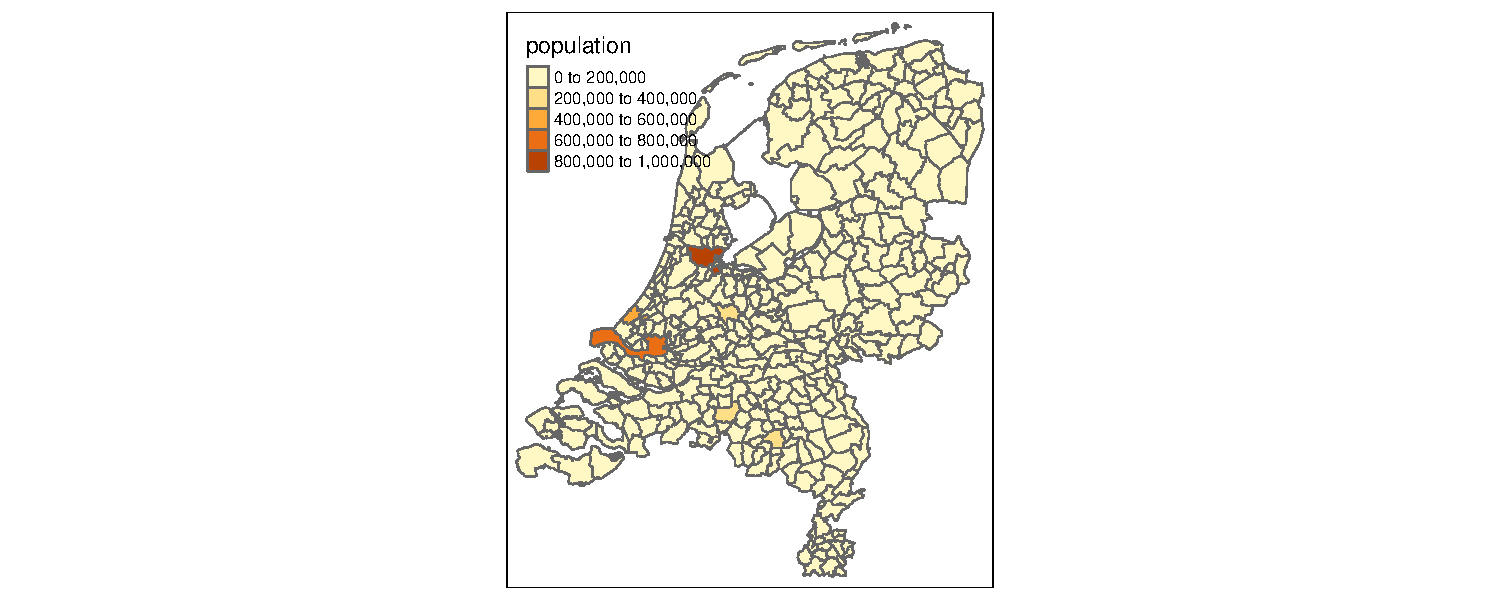
\includegraphics{slides_all2gether_part1_files/figure-beamer/unnamed-chunk-81-1.pdf}

\end{frame}

\begin{frame}[fragile]{Zwei Karten}

\begin{Shaded}
\begin{Highlighting}[]
\KeywordTok{tm_shape}\NormalTok{(Europe) }\OperatorTok{+}
\StringTok{    }\KeywordTok{tm_fill}\NormalTok{(}\KeywordTok{c}\NormalTok{(}\StringTok{"pop_est"}\NormalTok{, }\StringTok{"economy"}\NormalTok{), }
        \DataTypeTok{title=}\KeywordTok{c}\NormalTok{(}\StringTok{"Population"}\NormalTok{, }\StringTok{"Economy"}\NormalTok{))}
\end{Highlighting}
\end{Shaded}

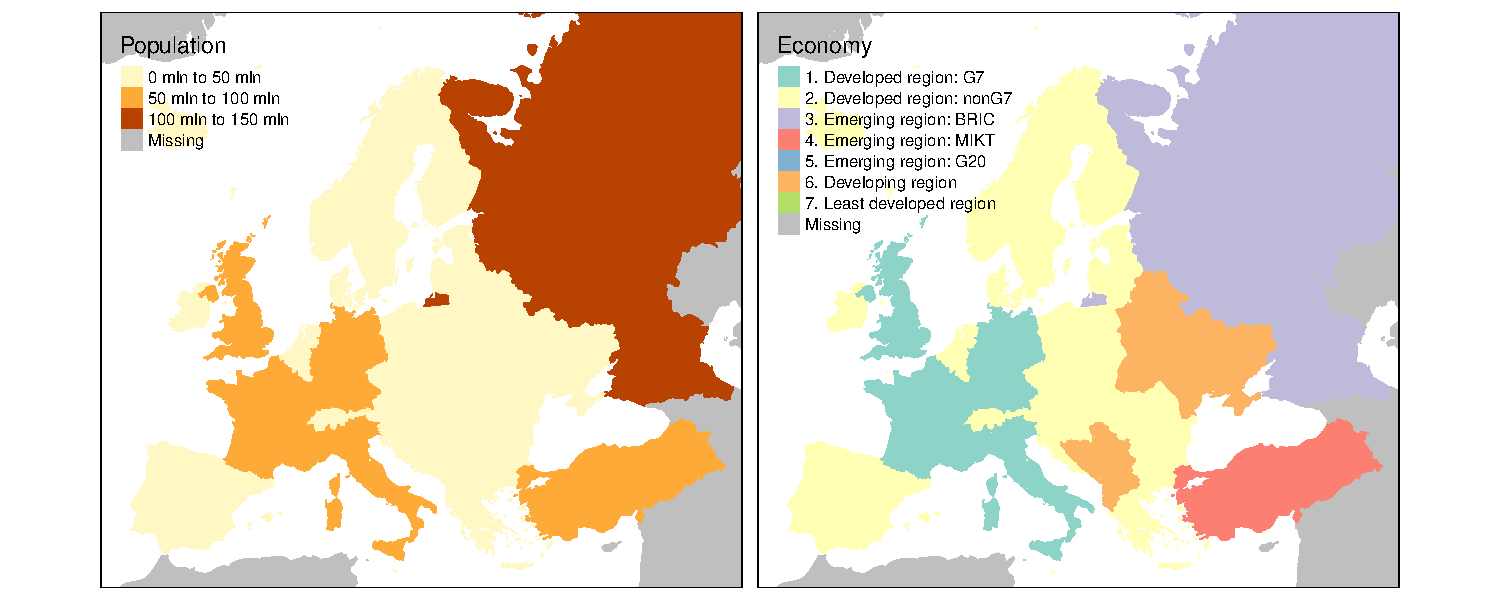
\includegraphics{slides_all2gether_part1_files/figure-beamer/unnamed-chunk-82-1.pdf}

\end{frame}

\begin{frame}[fragile]{Räumliche Daten zur Flächennutzung}

\begin{Shaded}
\begin{Highlighting}[]
\KeywordTok{data}\NormalTok{(land)}
\KeywordTok{data}\NormalTok{(World)}
\end{Highlighting}
\end{Shaded}

\begin{longtable}[]{@{}llr@{}}
\toprule
& cover\_cls & trees\tabularnewline
\midrule
\endhead
239644 & Water & NA\tabularnewline
184394 & Bare area/Sparse vegetation & 0\tabularnewline
306844 & Water & NA\tabularnewline
90696 & Forest & 14\tabularnewline
352519 & Water & NA\tabularnewline
546692 & Snow/ice & 0\tabularnewline
375559 & Water & NA\tabularnewline
158069 & Water & NA\tabularnewline
487509 & Water & NA\tabularnewline
25804 & Water & NA\tabularnewline
\bottomrule
\end{longtable}

\end{frame}

\begin{frame}[fragile]{Weltweite Flächennutzung}

\begin{Shaded}
\begin{Highlighting}[]
\KeywordTok{tm_shape}\NormalTok{(land,  }\DataTypeTok{relative=}\OtherTok{FALSE}\NormalTok{) }\OperatorTok{+}
\StringTok{    }\KeywordTok{tm_raster}\NormalTok{(}\StringTok{"trees"}\NormalTok{, }\DataTypeTok{title=}\StringTok{"Anteil Waldfläche"}\NormalTok{)}
\end{Highlighting}
\end{Shaded}

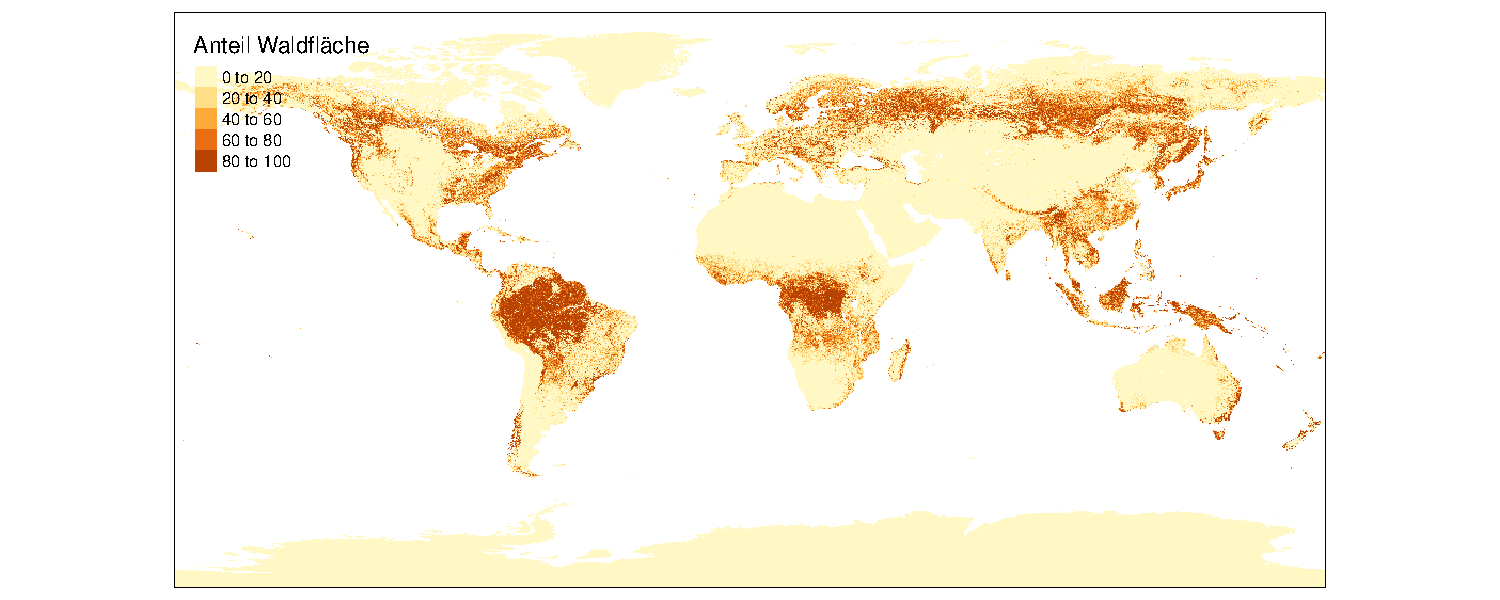
\includegraphics{slides_all2gether_part1_files/figure-beamer/unnamed-chunk-86-1.pdf}

\end{frame}

\begin{frame}[fragile]{Räumliche Daten zu Metropolregionen}

\begin{Shaded}
\begin{Highlighting}[]
\KeywordTok{data}\NormalTok{(metro)}
\end{Highlighting}
\end{Shaded}

\begin{longtable}[]{@{}llllrrrrrrrrr@{}}
\toprule
& name & name\_long & iso\_a3 & pop1950 & pop1960 & pop1970 & pop1980 &
pop1990 & pop2000 & pop2010 & pop2020 & pop2030\tabularnewline
\midrule
\endhead
2 & Kabul & Kabul & AFG & 170784 & 285352 & 471891 & 977824 & 1549320 &
2401109 & 3722320 & 5721697 & 8279607\tabularnewline
8 & Algiers & El Djazair (Algiers) & DZA & 516450 & 871636 & 1281127 &
1621442 & 1797068 & 2140577 & 2432023 & 2835218 & 3404575\tabularnewline
13 & Luanda & Luanda & AGO & 138413 & 219427 & 459225 & 771349 & 1390240
& 2591388 & 4508434 & 6836849 & 10428756\tabularnewline
16 & Buenos Aires & Buenos Aires & ARG & 5097612 & 6597634 & 8104621 &
9422362 & 10513284 & 12406780 & 14245871 & 15894307 &
16956491\tabularnewline
17 & Cordoba & Cordoba & ARG & 429249 & 605309 & 809794 & 1009521 &
1200168 & 1347561 & 1459268 & 1562509 & 1718192\tabularnewline
25 & Rosario & Rosario & ARG & 554483 & 671349 & 816230 & 953491 &
1083819 & 1152387 & 1298073 & 1453814 & 1606993\tabularnewline
32 & Yerevan & Yerevan & ARM & 341432 & 537759 & 778158 & 1041587 &
1174524 & 1111301 & 1065597 & 1023703 & 1057459\tabularnewline
33 & Adelaide & Adelaide & AUS & 429277 & 571822 & 850168 & 971856 &
1081618 & 1141623 & 1217990 & 1320783 & 1505422\tabularnewline
34 & Brisbane & Brisbane & AUS & 441718 & 602999 & 904777 & 1134833 &
1381306 & 1666203 & 2033617 & 2388517 & 2721325\tabularnewline
37 & Melbourne & Melbourne & AUS & 1331966 & 1851220 & 2499109 & 2839019
& 3154314 & 3460541 & 3951216 & 4500501 & 5070873\tabularnewline
\bottomrule
\end{longtable}

\end{frame}

\begin{frame}[fragile]{Nur ein Land visualisieren}

\begin{Shaded}
\begin{Highlighting}[]
\KeywordTok{tm_shape}\NormalTok{(Europe[Europe}\OperatorTok{$}\NormalTok{name}\OperatorTok{==}\StringTok{"Austria"}\NormalTok{, ]) }\OperatorTok{+}
\StringTok{    }\KeywordTok{tm_polygons}\NormalTok{()}
\end{Highlighting}
\end{Shaded}

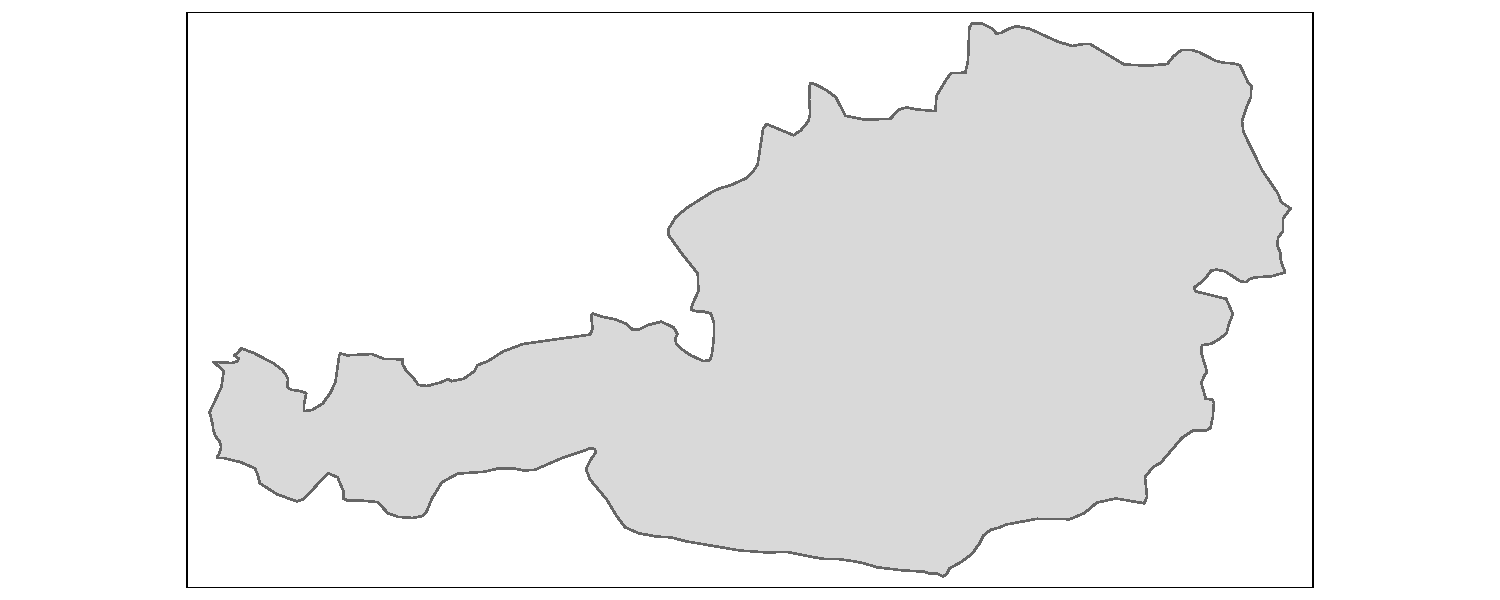
\includegraphics{slides_all2gether_part1_files/figure-beamer/unnamed-chunk-90-1.pdf}

\end{frame}

\begin{frame}[fragile]{Beispieldaten laden}

\begin{block}{Datenquelle Eurostat}

\begin{itemize}
\tightlist
\item
  Daten zur Arbeitslosigkeit in Europa
\end{itemize}

\begin{Shaded}
\begin{Highlighting}[]
\NormalTok{url <-}\StringTok{ "https://raw.githubusercontent.com/Japhilko/}
\StringTok{GeoData/master/2015/data/Unemployment07a13.csv"}

\NormalTok{Unemp <-}\StringTok{ }\KeywordTok{read.csv}\NormalTok{(url) }
\end{Highlighting}
\end{Shaded}

\end{block}

\end{frame}

\begin{frame}{Überblick über die Daten}

\begin{longtable}[]{@{}rlrr@{}}
\toprule
X & GEO & Val2007M12 & Val2013M01\tabularnewline
\midrule
\endhead
9316 & EU28 & 6.9 & 10.9\tabularnewline
9325 & EU27 & 6.9 & 10.9\tabularnewline
9334 & EU25 & 6.9 & 11.0\tabularnewline
9343 & EU15 & 6.9 & 11.1\tabularnewline
9352 & EA & 7.3 & 12.0\tabularnewline
9361 & EA19 & 7.3 & 12.0\tabularnewline
9370 & EA18 & 7.4 & 12.0\tabularnewline
9379 & EA17 & 7.4 & 12.0\tabularnewline
9388 & EA16 & 7.4 & 12.0\tabularnewline
9397 & EA15 & 7.3 & 12.0\tabularnewline
\bottomrule
\end{longtable}

\end{frame}

\begin{frame}[fragile]{Nutzung des Paketes \texttt{tmap} mit eigenen
Daten}

\begin{Shaded}
\begin{Highlighting}[]
\KeywordTok{library}\NormalTok{(}\StringTok{"tmap"}\NormalTok{)}
\KeywordTok{data}\NormalTok{(Europe)}
\end{Highlighting}
\end{Shaded}

\begin{block}{Die Daten matchen}

\begin{Shaded}
\begin{Highlighting}[]
\NormalTok{iso_a2<-}\StringTok{ }\KeywordTok{substr}\NormalTok{(Europe}\OperatorTok{@}\NormalTok{data}\OperatorTok{$}\NormalTok{iso_a3,}\DecValTok{1}\NormalTok{,}\DecValTok{2}\NormalTok{)}
\NormalTok{ind <-}\StringTok{ }\KeywordTok{match}\NormalTok{(iso_a2,Unemp}\OperatorTok{$}\NormalTok{GEO)}
\NormalTok{Europe}\OperatorTok{@}\NormalTok{data}\OperatorTok{$}\NormalTok{Val2007M12 <-}\StringTok{ }\NormalTok{Unemp}\OperatorTok{$}\NormalTok{Val2007M12[ind]}
\NormalTok{Europe}\OperatorTok{@}\NormalTok{data}\OperatorTok{$}\NormalTok{Val2013M01 <-}\StringTok{ }\NormalTok{Unemp}\OperatorTok{$}\NormalTok{Val2013M01[ind]}
\end{Highlighting}
\end{Shaded}

\end{block}

\end{frame}

\begin{frame}[fragile]{Eine Karte erzeugen}

\begin{Shaded}
\begin{Highlighting}[]
\KeywordTok{qtm}\NormalTok{(Europe,}\KeywordTok{c}\NormalTok{(}\StringTok{"Val2007M12"}\NormalTok{,}\StringTok{"Val2013M01"}\NormalTok{))}
\end{Highlighting}
\end{Shaded}

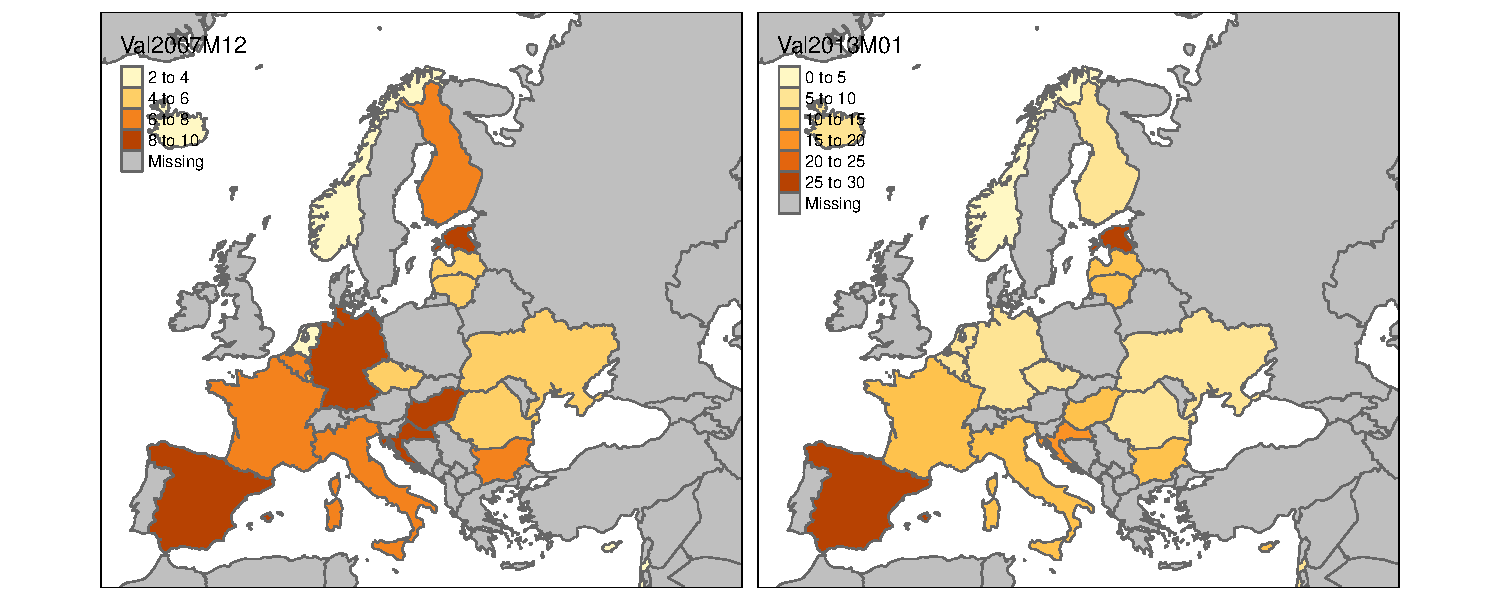
\includegraphics{slides_all2gether_part1_files/figure-beamer/unnamed-chunk-95-1.pdf}

\end{frame}

\begin{frame}[fragile]{Kleine und viele Karten}

\begin{Shaded}
\begin{Highlighting}[]
\KeywordTok{tm_shape}\NormalTok{(Europe[Europe}\OperatorTok{$}\NormalTok{continent}\OperatorTok{==}\StringTok{"Europe"}\NormalTok{,]) }\OperatorTok{+}
\StringTok{    }\KeywordTok{tm_fill}\NormalTok{(}\StringTok{"part"}\NormalTok{, }\DataTypeTok{thres.poly =} \DecValTok{0}\NormalTok{) }\OperatorTok{+}
\StringTok{    }\KeywordTok{tm_facets}\NormalTok{(}\StringTok{"name"}\NormalTok{, }\DataTypeTok{free.coords=}\OtherTok{TRUE}\NormalTok{)}
\end{Highlighting}
\end{Shaded}

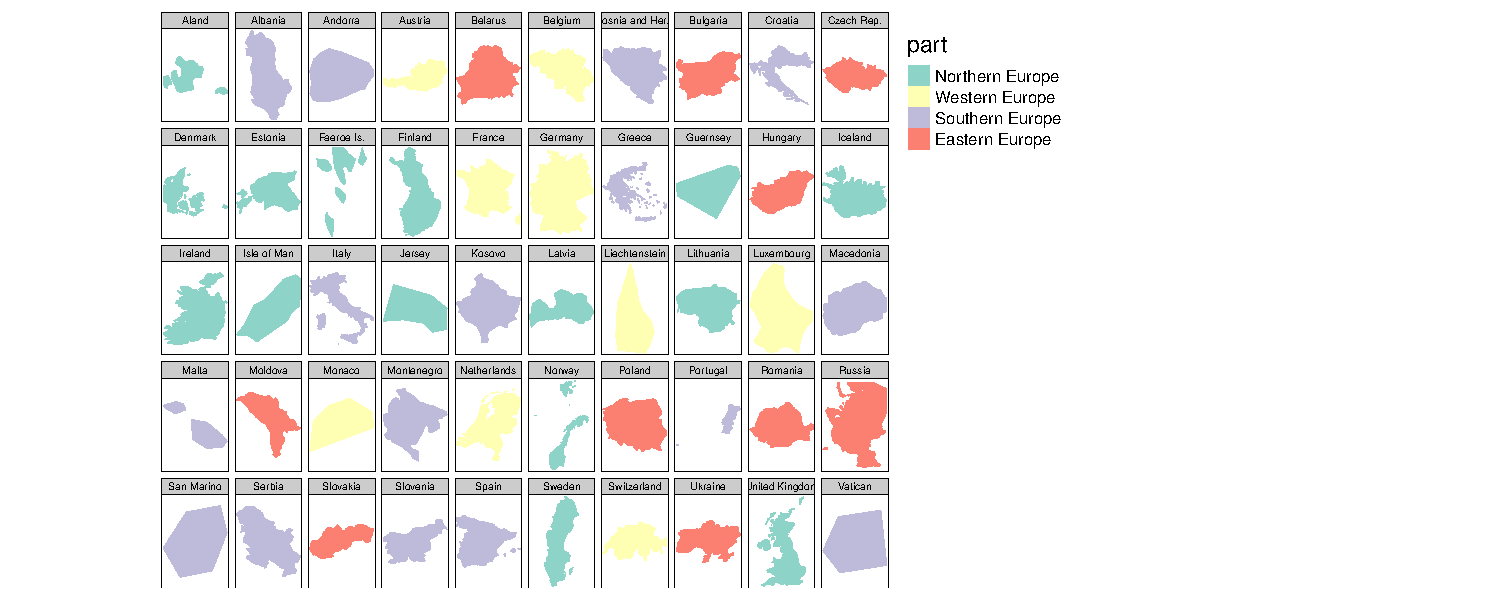
\includegraphics{slides_all2gether_part1_files/figure-beamer/unnamed-chunk-97-1.pdf}

\end{frame}

\begin{frame}[fragile]{tmap zitieren}

\begin{Shaded}
\begin{Highlighting}[]
\KeywordTok{citation}\NormalTok{(}\StringTok{"tmap"}\NormalTok{)}
\end{Highlighting}
\end{Shaded}

\begin{verbatim}
## 
## To cite tmap/tmaptools in publications use:
## 
## Tennekes M (2018). "tmap: Thematic Maps in R." _Journal of
## Statistical Software_, *84*(6), 1-39. doi: 10.18637/jss.v084.i06
## (URL: http://doi.org/10.18637/jss.v084.i06).
## 
## A BibTeX entry for LaTeX users is
## 
##   @Article{,
##     title = {{tmap}: Thematic Maps in {R}},
##     author = {Martijn Tennekes},
##     journal = {Journal of Statistical Software},
##     year = {2018},
##     volume = {84},
##     number = {6},
##     pages = {1--39},
##     doi = {10.18637/jss.v084.i06},
##   }
\end{verbatim}

\end{frame}

\begin{frame}[fragile]{Inhalt dieses Abschnitts}

\begin{itemize}
\tightlist
\item
  Der Beispieldatensatz \texttt{wrld\_simpl} im Paket \texttt{maptools}
  wird vorgestellt.
\item
  Es wird gezeigt, wie man Daten aus anderen Quellen mit Kartendaten
  verbinden kann.
\item
  Mit dieser Verbindung ist es dann möglich thematische Karten - so
  genannte Choroplethen - zu erstellen
\item
  Zudem wird das Paket \texttt{choroplethr} vorgestellt.
\end{itemize}

\end{frame}

\begin{frame}{Was ist ein Choropleth}

Ein Choropleth ist eine Karte, die

\begin{itemize}
\tightlist
\item
  geografische Grenzen zeigt.
\item
  bei denen Bereiche basierend auf Metriken eingefärbt werden.
\end{itemize}

Choroplethen sind nützlich für die Visualisierung von Daten, wo
geografische Grenzen eine natürliche Einheit der Aggregation sind.

\end{frame}

\begin{frame}[fragile]{Das Paket \texttt{maptools}}

\begin{itemize}
\tightlist
\item
  Datensatz wrld\_simpl aus dem Paket \texttt{maptools}
\item
  Polygone für fast alle Staaten der Erde
\end{itemize}

\begin{Shaded}
\begin{Highlighting}[]
\KeywordTok{library}\NormalTok{(maptools)}
\KeywordTok{data}\NormalTok{(wrld_simpl)}
\end{Highlighting}
\end{Shaded}

\begin{longtable}[]{@{}lllrr@{}}
\toprule
& ISO2 & NAME & AREA & POP2005\tabularnewline
\midrule
\endhead
ATG & AG & Antigua and Barbuda & 44 & 83039\tabularnewline
DZA & DZ & Algeria & 238174 & 32854159\tabularnewline
AZE & AZ & Azerbaijan & 8260 & 8352021\tabularnewline
ALB & AL & Albania & 2740 & 3153731\tabularnewline
ARM & AM & Armenia & 2820 & 3017661\tabularnewline
AGO & AO & Angola & 124670 & 16095214\tabularnewline
\bottomrule
\end{longtable}

\end{frame}

\begin{frame}[fragile]{Hallo Welt}

\begin{Shaded}
\begin{Highlighting}[]
\KeywordTok{plot}\NormalTok{(wrld_simpl)}
\end{Highlighting}
\end{Shaded}

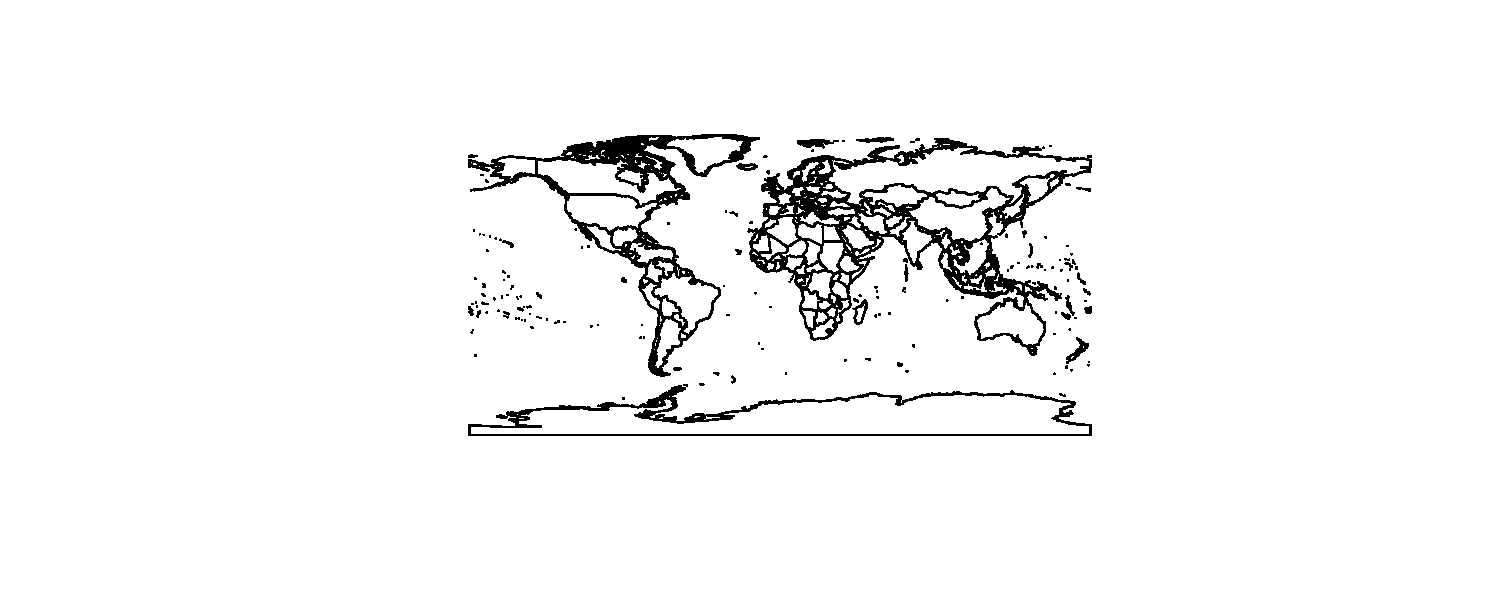
\includegraphics{slides_all2gether_part1_files/figure-beamer/unnamed-chunk-104-1.pdf}

\end{frame}

\begin{frame}[fragile]{\href{https://datahub.io/core/gini-index\#data}{Daten
zum Gini Index}}

\begin{itemize}
\tightlist
\item
  Daten von
  \href{https://datahub.io/core/gini-index\#data}{\textbf{datahub.io}}
\item
  Statistisches Maß zur Darstellung von
  \href{https://de.wikipedia.org/wiki/Gini-Koeffizient}{Ungleichverteilungen}
\end{itemize}

\begin{Shaded}
\begin{Highlighting}[]
\NormalTok{gini <-}\StringTok{ }\KeywordTok{read.csv}\NormalTok{(}\StringTok{"../data/gini-index_csv.csv"}\NormalTok{)}
\end{Highlighting}
\end{Shaded}

\begin{longtable}[]{@{}llrr@{}}
\toprule
Country.Name & Country.Code & Year & Value\tabularnewline
\midrule
\endhead
Albania & ALB & 1996 & 27.0\tabularnewline
Albania & ALB & 2002 & 31.7\tabularnewline
Albania & ALB & 2005 & 30.6\tabularnewline
Albania & ALB & 2008 & 30.0\tabularnewline
Albania & ALB & 2012 & 29.0\tabularnewline
Algeria & DZA & 1988 & 40.2\tabularnewline
\bottomrule
\end{longtable}

\end{frame}

\begin{frame}[fragile]{Der Gini Index im Jahr 2012}

\begin{itemize}
\tightlist
\item
  Für das Jahr 2012 sind am meisten Beobachtungen vorhanden.
\end{itemize}

\begin{Shaded}
\begin{Highlighting}[]
\NormalTok{gini12 <-}\StringTok{ }\NormalTok{gini[gini}\OperatorTok{$}\NormalTok{Year}\OperatorTok{==}\DecValTok{2012}\NormalTok{,]}
\KeywordTok{summary}\NormalTok{(gini12}\OperatorTok{$}\NormalTok{Value)}
\end{Highlighting}
\end{Shaded}

\begin{verbatim}
##    Min. 1st Qu.  Median    Mean 3rd Qu.    Max. 
##   24.70   29.80   35.10   36.15   41.40   57.40
\end{verbatim}

\end{frame}

\begin{frame}[fragile]{Exkurs: der Befehl \texttt{match}}

\begin{Shaded}
\begin{Highlighting}[]
\NormalTok{vec_a <-}\StringTok{ }\KeywordTok{c}\NormalTok{(}\StringTok{"A"}\NormalTok{,}\DecValTok{2}\NormalTok{,}\DecValTok{6}\NormalTok{,}\DecValTok{1}\NormalTok{,}\StringTok{"C"}\NormalTok{)}
\NormalTok{vec_b <-}\StringTok{ }\KeywordTok{c}\NormalTok{(}\DecValTok{1}\NormalTok{,}\StringTok{"C"}\NormalTok{,}\DecValTok{2}\NormalTok{)}

\KeywordTok{match}\NormalTok{(vec_a,vec_b)}
\end{Highlighting}
\end{Shaded}

\begin{verbatim}
## [1] NA  3 NA  1  2
\end{verbatim}

\end{frame}

\begin{frame}[fragile]{Die Daten matchen}

\begin{itemize}
\tightlist
\item
  WIr matchen die Gini-Daten mit den Kartendaten
\end{itemize}

\begin{Shaded}
\begin{Highlighting}[]
\NormalTok{ind <-}\StringTok{ }\KeywordTok{match}\NormalTok{(gini12}\OperatorTok{$}\NormalTok{Country.Code,wrld_simpl}\OperatorTok{$}\NormalTok{ISO3)}
\end{Highlighting}
\end{Shaded}

\begin{itemize}
\tightlist
\item
  Wir nehmen die Länder raus, für die keine Daten vorhanden sind:
\end{itemize}

\begin{Shaded}
\begin{Highlighting}[]
\NormalTok{ind2 <-}\StringTok{ }\NormalTok{ind[}\OperatorTok{!}\KeywordTok{is.na}\NormalTok{(ind)]}
\end{Highlighting}
\end{Shaded}

\begin{itemize}
\tightlist
\item
  Eine neue Karte wird erstellt:
\end{itemize}

\begin{Shaded}
\begin{Highlighting}[]
\NormalTok{ginimap <-}\StringTok{ }\NormalTok{wrld_simpl[ind2,]}
\end{Highlighting}
\end{Shaded}

\begin{itemize}
\tightlist
\item
  Die Gini-Daten werden in den Datenslot geschrieben
\end{itemize}

\begin{Shaded}
\begin{Highlighting}[]
\NormalTok{ginimap}\OperatorTok{@}\NormalTok{data}\OperatorTok{$}\NormalTok{gini12 <-}\StringTok{ }\NormalTok{gini12}\OperatorTok{$}\NormalTok{Value[}\OperatorTok{!}\KeywordTok{is.na}\NormalTok{(ind)]}
\end{Highlighting}
\end{Shaded}

\end{frame}

\begin{frame}[fragile]{Die Daten plotten}

\begin{Shaded}
\begin{Highlighting}[]
\KeywordTok{library}\NormalTok{(sp)}
\KeywordTok{spplot}\NormalTok{(ginimap,}\StringTok{"gini12"}\NormalTok{)}
\end{Highlighting}
\end{Shaded}

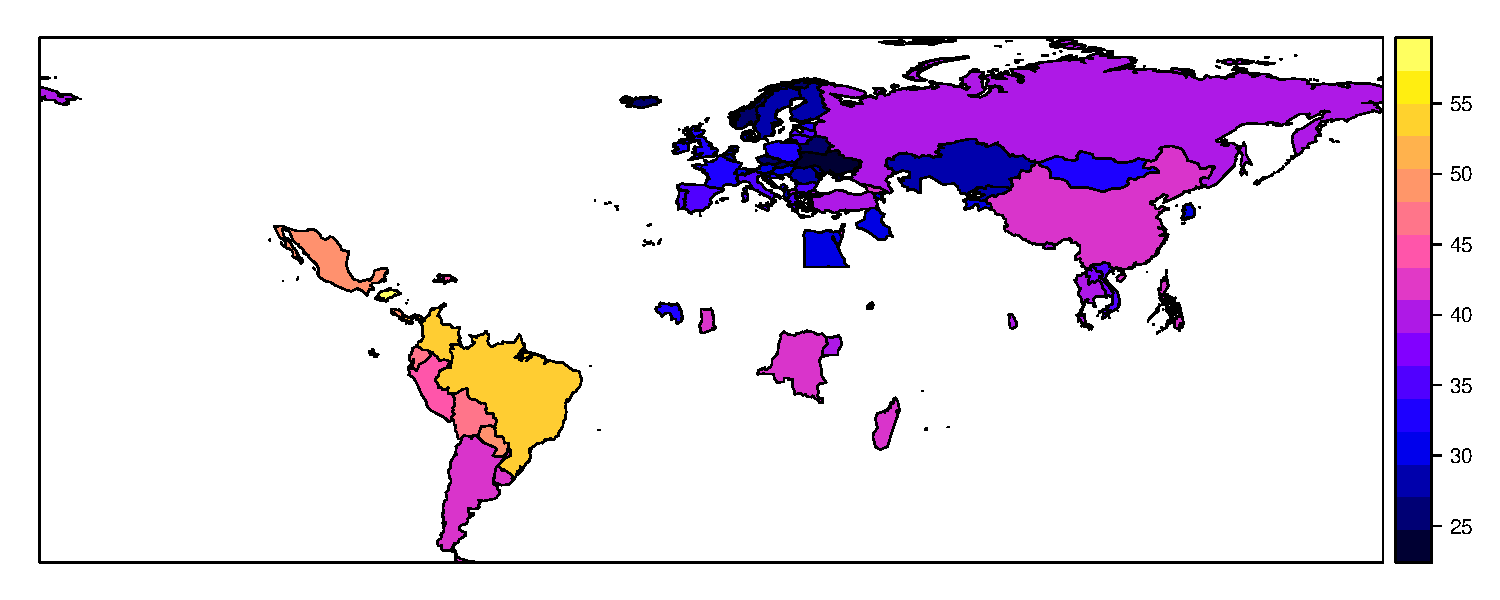
\includegraphics{slides_all2gether_part1_files/figure-beamer/unnamed-chunk-113-1.pdf}

\end{frame}

\begin{frame}[fragile]{Aufgabe A4A - Eine Choroplethenkarte erzeugen}

\begin{itemize}
\tightlist
\item
  Lade Datensatz
  \href{https://raw.githubusercontent.com/Japhilko/GeoData/master/2015/data/Unemployment.csv}{\textbf{Unemployment
  Datensatz}} herunter
\item
  Matche die Daten mit einer passenden Karte
\item
  Erzeuge mit der (Variable \texttt{X2014M10}) folgende Karte:
\end{itemize}

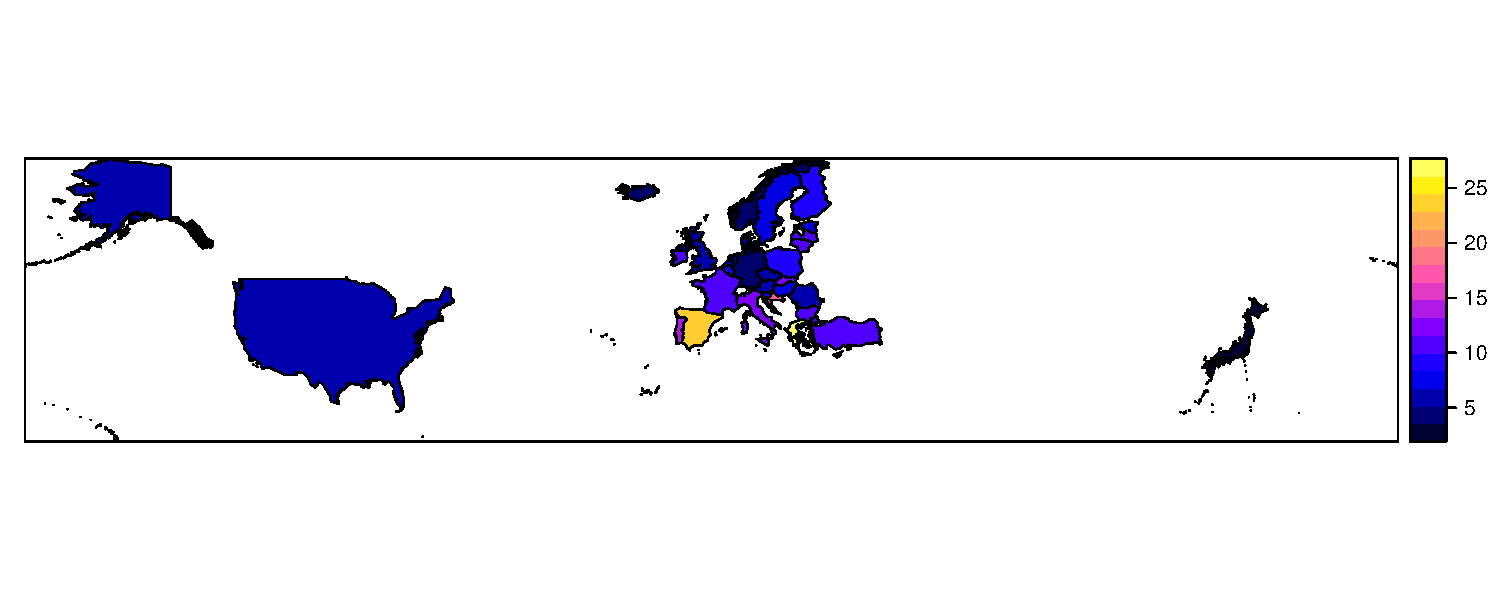
\includegraphics{slides_all2gether_part1_files/figure-beamer/unnamed-chunk-114-1.pdf}

\end{frame}

\begin{frame}[fragile]{Das Paket \texttt{choroplethr}}

\begin{block}{Paket von \href{http://www.arilamstein.com/}{\textbf{Ari
Lamstein}} -
\href{https://cran.r-project.org/web/packages/choroplethr/index.html}{\textbf{\texttt{choroplethr}}}}

\begin{itemize}
\item
  Vereinfachung der Erstellung von Choroplethen in R
\item
  World Development Indicators
  \href{https://cran.r-project.org/web/packages/WDI/index.html}{\textbf{\texttt{WDI}}}
  (World Bank)
\item
  Die folgenden Beispiele basieren auf der
  \href{https://cran.r-project.org/web/packages/choroplethr/index.html}{\textbf{Vignette}}
  des \texttt{choroplethr}-Paketes
\end{itemize}

\begin{Shaded}
\begin{Highlighting}[]
\KeywordTok{install.packages}\NormalTok{(}\StringTok{"choroplethr"}\NormalTok{)}
\end{Highlighting}
\end{Shaded}

\end{block}

\end{frame}

\begin{frame}[fragile]{Bevölkerungsschätzungen für den US-Staaten}

\texttt{df\_pop\_state} ist ein Datensatz , der in dem Paket
\texttt{choroplethr} enthalten ist, es enthält Schätzungen zu den
US-Staaten für das Jahr 2012.

\begin{longtable}[]{@{}lr@{}}
\toprule
region & value\tabularnewline
\midrule
\endhead
alabama & 4777326\tabularnewline
alaska & 711139\tabularnewline
arizona & 6410979\tabularnewline
arkansas & 2916372\tabularnewline
california & 37325068\tabularnewline
colorado & 5042853\tabularnewline
\bottomrule
\end{longtable}

\end{frame}

\begin{frame}[fragile]{\texttt{choroplethr} -
\href{http://mirrors.softliste.de/cran/web/packages/choroplethr/vignettes/a-introduction.html}{Hallo
Welt}}

Die Karte zeigt die US Bevölkerungsschätzung für die US-Staaten und das
Jahr 2012:

Wir bekommen eine Choroplethenkarte mit nur einem Argument:

\begin{Shaded}
\begin{Highlighting}[]
\KeywordTok{state_choropleth}\NormalTok{(df_pop_state)}
\end{Highlighting}
\end{Shaded}

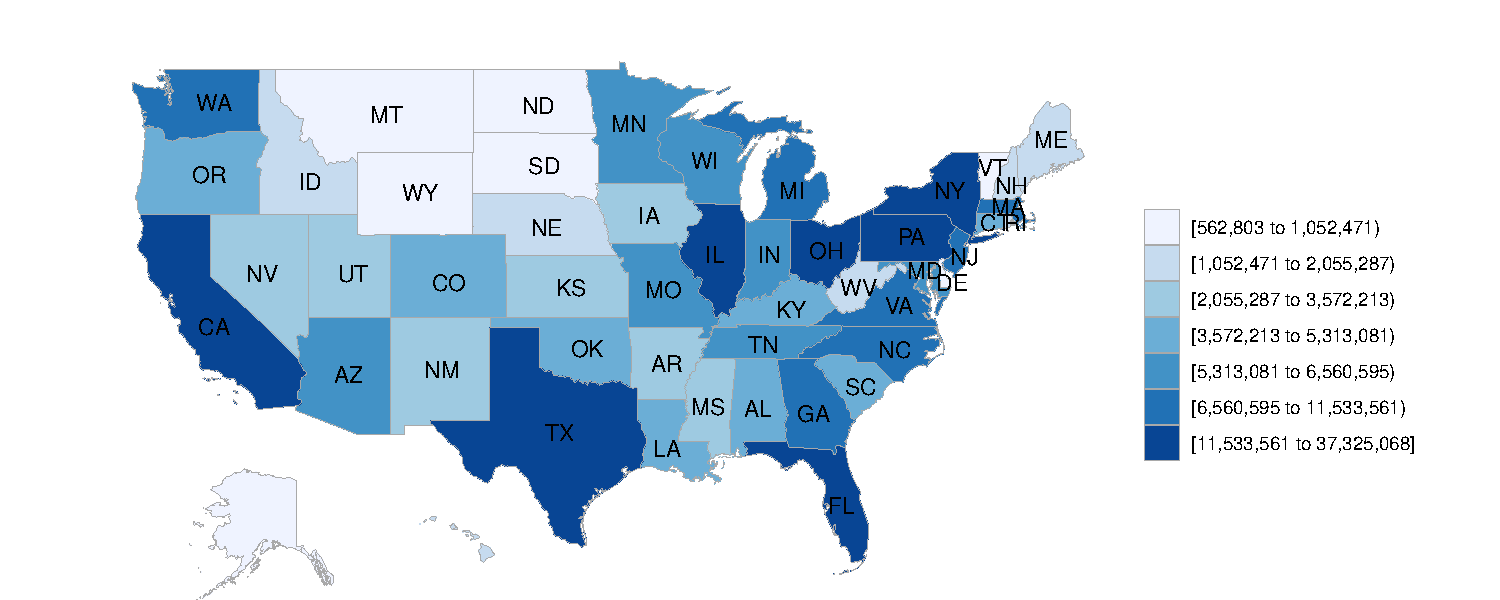
\includegraphics{slides_all2gether_part1_files/figure-beamer/unnamed-chunk-120-1.pdf}

Aber wir können auch einen Titel erstellen und die Legende benennen:

\begin{Shaded}
\begin{Highlighting}[]
\KeywordTok{state_choropleth}\NormalTok{(df_pop_state, }\DataTypeTok{title=}\StringTok{"2012 US State Population Estimates"}\NormalTok{, }\DataTypeTok{legend=}\StringTok{"Population"}\NormalTok{)}
\end{Highlighting}
\end{Shaded}

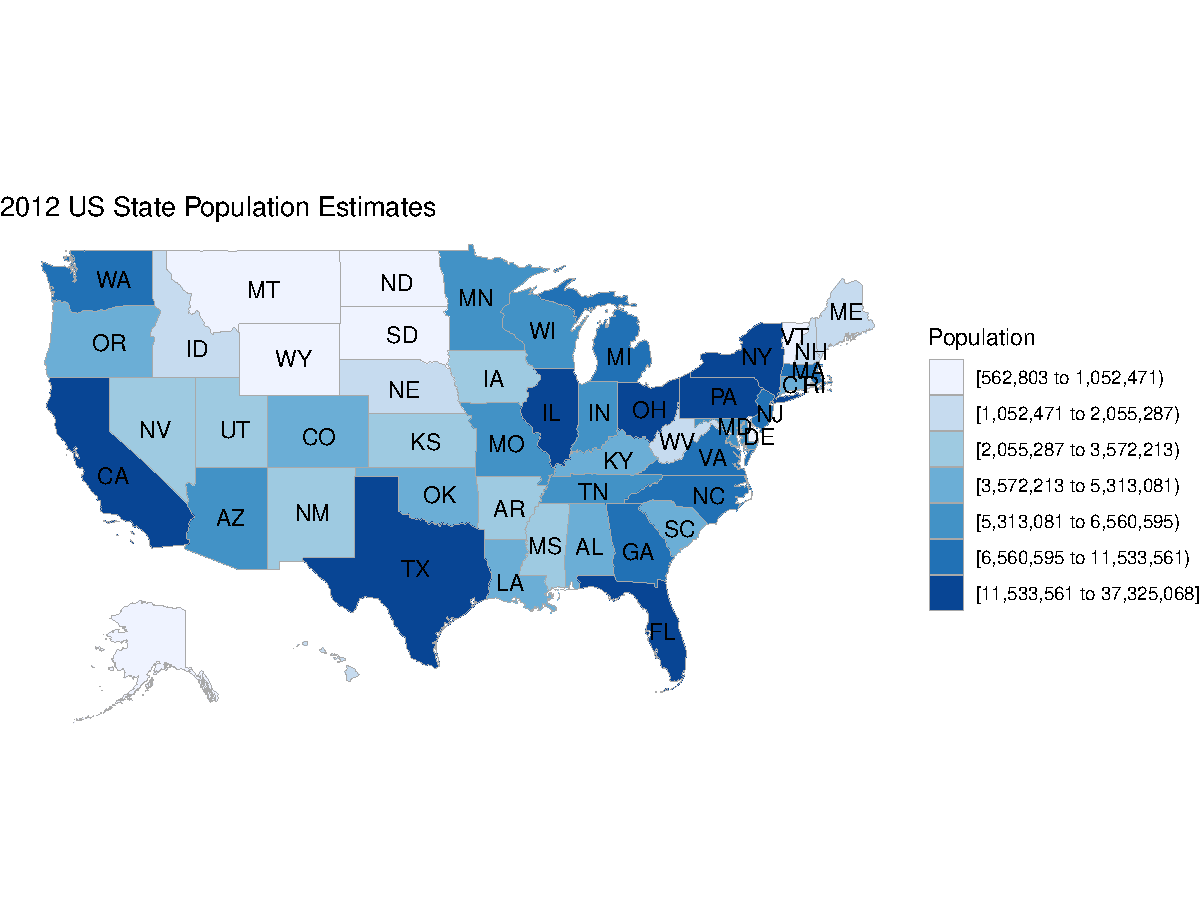
\includegraphics{slides_all2gether_part1_files/figure-beamer/unnamed-chunk-121-1.pdf}

\end{frame}

\begin{frame}[fragile]{\href{http://mirrors.softliste.de/cran/web/packages/choroplethr/vignettes/b-state-choropleth.html}{Nur
drei Staaten darstellen}}

\begin{Shaded}
\begin{Highlighting}[]
\KeywordTok{state_choropleth}\NormalTok{(df_pop_state,}
                 \DataTypeTok{title=} \StringTok{"2012 Population Estimates"}\NormalTok{,}
                 \DataTypeTok{legend=} \StringTok{"Population"}\NormalTok{, }\DataTypeTok{num_colors =} \DecValTok{1}\NormalTok{,}
                 \DataTypeTok{zoom=}\KeywordTok{c}\NormalTok{(}\StringTok{"california"}\NormalTok{,}\StringTok{"washington"}\NormalTok{,}\StringTok{"oregon"}\NormalTok{))}
\end{Highlighting}
\end{Shaded}

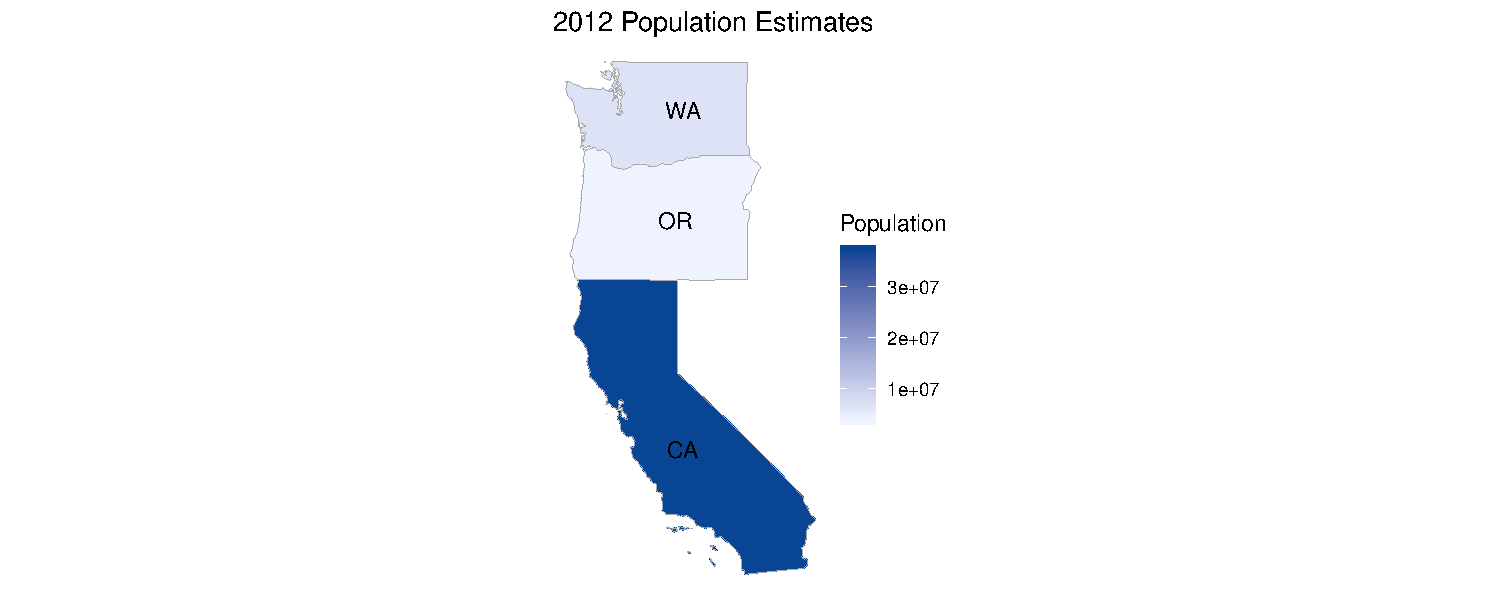
\includegraphics{slides_all2gether_part1_files/figure-beamer/unnamed-chunk-122-1.pdf}

\end{frame}

\begin{frame}[fragile]{US County Chroplethen}

\begin{block}{\href{http://mirrors.softliste.de/cran/web/packages/choroplethr/vignettes/c-county-choropleth.html}{Choroplethen
der US Counties}}

\begin{itemize}
\tightlist
\item
  \href{http://mirrors.softliste.de/cran/web/packages/choroplethr/vignettes/c-county-choropleth.html}{\textbf{Vignette
  des Pakets}}
\end{itemize}

\begin{Shaded}
\begin{Highlighting}[]
\CommentTok{# A data.frame containing population estimates for US Counties in 2012.}
\NormalTok{?df_pop_county}

\CommentTok{# Create a choropleth of US Counties}
\NormalTok{?county_choropleth}
\end{Highlighting}
\end{Shaded}

\end{block}

\end{frame}

\begin{frame}[fragile]{Eine Karte der US Counties}

\begin{Shaded}
\begin{Highlighting}[]
\KeywordTok{data}\NormalTok{(df_pop_county)}
\KeywordTok{county_choropleth}\NormalTok{(df_pop_county)}
\end{Highlighting}
\end{Shaded}

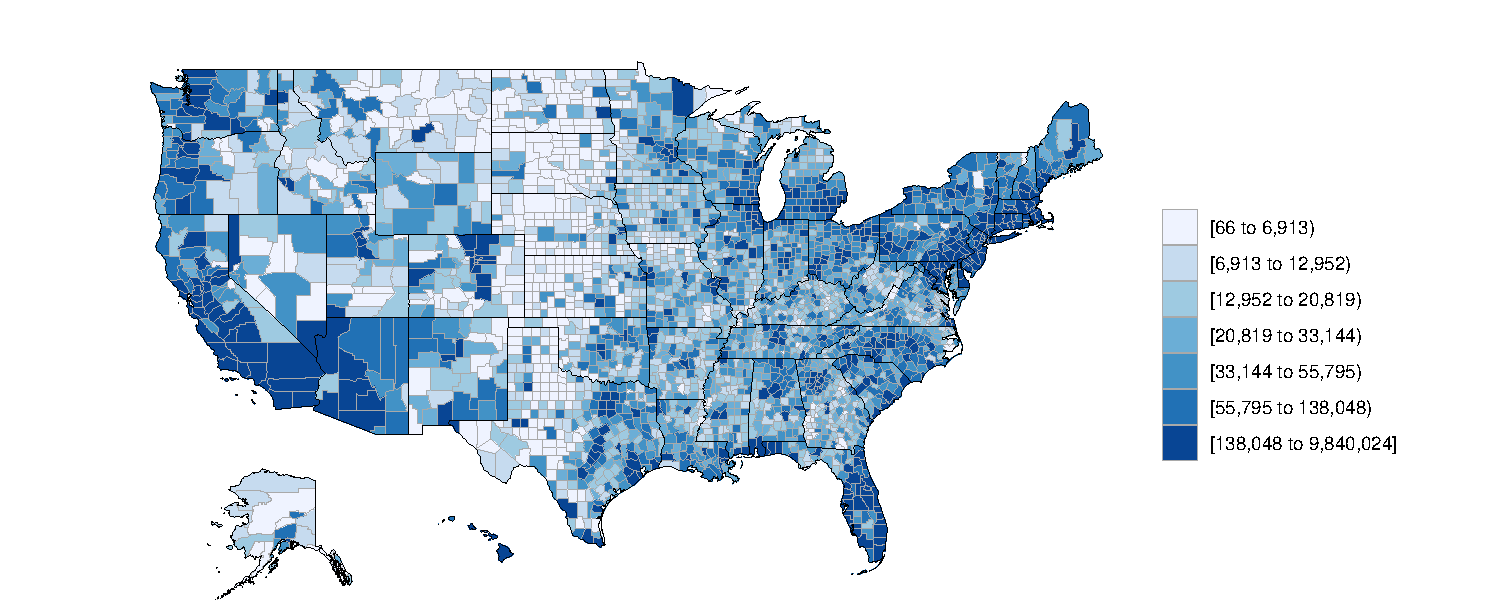
\includegraphics{slides_all2gether_part1_files/figure-beamer/unnamed-chunk-124-1.pdf}

\end{frame}

\begin{frame}[fragile]{\href{http://mirrors.softliste.de/cran/web/packages/choroplethr/vignettes/d-country-choropleth.html}{Choroplethen
Länder}}

\begin{Shaded}
\begin{Highlighting}[]
\KeywordTok{data}\NormalTok{(df_pop_country)}
\KeywordTok{country_choropleth}\NormalTok{(df_pop_country,}
              \DataTypeTok{title      =} \StringTok{"2012 Population Estimates"}\NormalTok{,}
              \DataTypeTok{legend     =} \StringTok{"Population"}\NormalTok{,}
              \DataTypeTok{num_colors =} \DecValTok{1}\NormalTok{,}
              \DataTypeTok{zoom       =} \KeywordTok{c}\NormalTok{(}\StringTok{"united states of america"}\NormalTok{,}
                             \StringTok{"mexico"}\NormalTok{, }\StringTok{"canada"}\NormalTok{))}
\end{Highlighting}
\end{Shaded}

\end{frame}

\begin{frame}{\href{http://mirrors.softliste.de/cran/web/packages/choroplethr/vignettes/d-country-choropleth.html}{Choroplethen
Länder}}

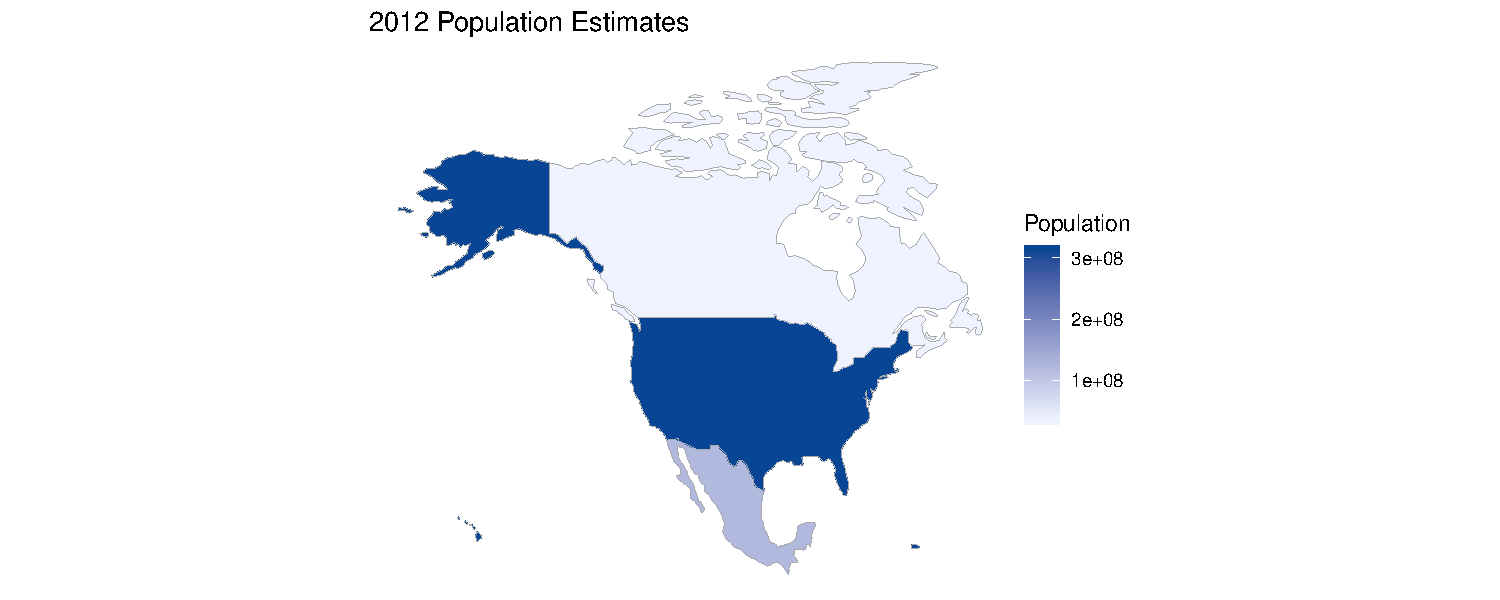
\includegraphics{slides_all2gether_part1_files/figure-beamer/unnamed-chunk-126-1.pdf}

\end{frame}

\begin{frame}[fragile]{Weltbank Daten}

\begin{Shaded}
\begin{Highlighting}[]
\KeywordTok{library}\NormalTok{(WDI) }
\KeywordTok{choroplethr_wdi}\NormalTok{(}\DataTypeTok{code=}\StringTok{"SP.POP.TOTL"}\NormalTok{, }\DataTypeTok{year=}\DecValTok{2012}\NormalTok{, }
                \DataTypeTok{title=}\StringTok{"2012 Population"}\NormalTok{, }
                \DataTypeTok{num_colors=}\DecValTok{1}\NormalTok{)}
\end{Highlighting}
\end{Shaded}

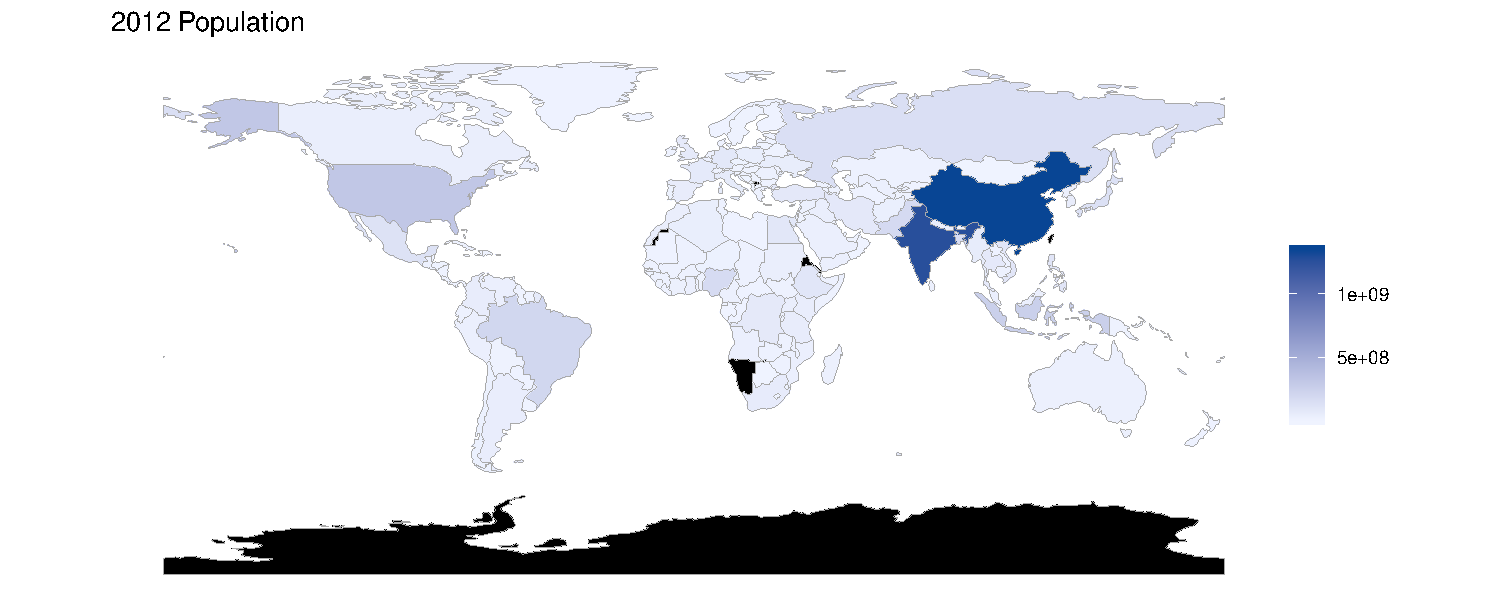
\includegraphics{slides_all2gether_part1_files/figure-beamer/unnamed-chunk-127-1.pdf}

\end{frame}

\begin{frame}[fragile]{\href{http://mirrors.softliste.de/cran/web/packages/choroplethr/vignettes/f-world-bank-data.html}{Lebenserwartung}}

\begin{Shaded}
\begin{Highlighting}[]
\KeywordTok{choroplethr_wdi}\NormalTok{(}\DataTypeTok{code=}\StringTok{"SP.DYN.LE00.IN"}\NormalTok{, }\DataTypeTok{year=}\DecValTok{2012}\NormalTok{,}
                \DataTypeTok{title=}\StringTok{"2012 Life Expectancy"}\NormalTok{)}
\end{Highlighting}
\end{Shaded}

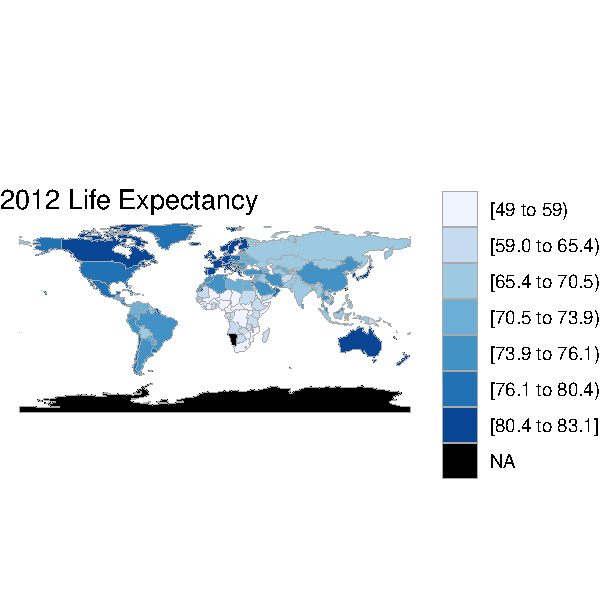
\includegraphics{slides_all2gether_part1_files/figure-beamer/unnamed-chunk-128-1.pdf}

\end{frame}

\begin{frame}[fragile]{Ein weiterer Datensatz}

\begin{quote}
A data.frame containing all US presdiential election results from 1789
to 2012
\end{quote}

\begin{Shaded}
\begin{Highlighting}[]
\KeywordTok{data}\NormalTok{(df_president_ts)}
\end{Highlighting}
\end{Shaded}

D = Democratic; R = Republican; PR = Progressive;

\begin{longtable}[]{@{}lllllllll@{}}
\toprule
& region & 1908 & 1912 & 1916 & 1920 & 1924 & 1928 & 1932\tabularnewline
\midrule
\endhead
42 & south dakota & R & PR & R & R & R & R & D\tabularnewline
43 & tennessee & D & D & D & R & D & R & D\tabularnewline
44 & texas & D & D & D & D & D & R & D\tabularnewline
45 & utah & R & R & D & R & R & R & D\tabularnewline
46 & vermont & R & R & R & R & R & R & R\tabularnewline
47 & virginia & D & D & D & D & D & R & D\tabularnewline
48 & washington & R & PR & D & R & R & R & D\tabularnewline
\bottomrule
\end{longtable}

\begin{Shaded}
\begin{Highlighting}[]
\CommentTok{# install.packages("choroplethrMaps")}
\KeywordTok{library}\NormalTok{(}\StringTok{"choroplethrMaps"}\NormalTok{)}
\end{Highlighting}
\end{Shaded}

\end{frame}

\begin{frame}[fragile]{Resourcen}

\begin{Shaded}
\begin{Highlighting}[]
\KeywordTok{citation}\NormalTok{(}\StringTok{"choroplethr"}\NormalTok{)}
\end{Highlighting}
\end{Shaded}

\begin{verbatim}
## 
## To cite package 'choroplethr' in publications use:
## 
##   Ari Lamstein (2018). choroplethr: Simplify the Creation of
##   Choropleth Maps in R. R package version 3.6.3.
##   https://CRAN.R-project.org/package=choroplethr
## 
## A BibTeX entry for LaTeX users is
## 
##   @Manual{,
##     title = {choroplethr: Simplify the Creation of Choropleth Maps in R},
##     author = {Ari Lamstein},
##     year = {2018},
##     note = {R package version 3.6.3},
##     url = {https://CRAN.R-project.org/package=choroplethr},
##   }
\end{verbatim}

\end{frame}

\begin{frame}[fragile]{Resources / Links}

\begin{itemize}
\item
  \href{https://cran.r-project.org/web/packages/choroplethr/vignettes/a-introduction.html}{\textbf{Einführung
  - Was sind Choroplethen}}
\item
  \href{http://radar.oreilly.com/2014/01/new-choropleth-package-in-r.html}{\textbf{Beschreibung}}
  der Nutzung des \texttt{choroplethr} Paketes
\item
  Die
  \href{https://cran.r-project.org/web/packages/choroplethr/vignettes/b-state-choropleth.html}{\textbf{US
  Staaten}} plotten mit \texttt{choroplethr}
\item
  \href{https://cran.r-project.org/web/packages/choroplethr/vignettes/f-world-bank-data.html}{\textbf{Weltbankdaten
  in Karten darstellen}} mit \texttt{choroplethr}
\item
  \href{http://blog.revolutionanalytics.com/2014/01/easy-data-maps-with-r-the-choroplethr-package-.html}{\textbf{Revolutions-Blog}}
  über das \texttt{choroplethr} Paket
\item
  \href{http://www.trulia.com/tech/2014/01/15/the-choroplethr-package-for-r/}{\textbf{trulia}}-blog
  über das \texttt{choroplethr} Paket
\item
  \href{http://www.r-bloggers.com/slides-for-my-upcoming-talk-mapping-census-data-in-r/}{\textbf{Präsentation
  von Ari Lamstein}} über das \texttt{choroplethr} Paket
\end{itemize}

\end{frame}

\begin{frame}{Worum geht es in diesem Abschnitt}

\begin{itemize}
\tightlist
\item
  Was sind Shapefiles
\item
  Shapefiles mit Vorwahl- und PLZ-Bereichen importieren
\item
  Einzelne Polygonzüge zusammenfassen
\item
  Adressen für die gezogenen Punkte bestimmen
\item
  Adressdatensatz bereinigen
\item
  Entfernung zum Hauptbahnhof bestimmen
\end{itemize}

\end{frame}

\begin{frame}{Das shapefile Format \ldots{}}

\begin{itemize}
\item
  \ldots{} ist ein beliebtes Format räumlicher Vektordaten für
  geographisches Informationssysteme (GIS).
\item
  Es wurde entwickelt und reguliert von
  \href{http://www.esri.com/}{ESRI}
\item
  (meist) offene Spezifikation um Daten Interoperabilität zwischen Esri
  und anderen Formaten zu sichern.
\item
  Es können Punkte, Linien und Polygone beschrieben werden
\item
  Jedes Element hat Attribute, wie bspw. Name oder Temperatur die es
  beschreiben.
\end{itemize}

Quelle: \url{https://en.wikipedia.org/wiki/Shapefile}

\end{frame}

\begin{frame}{Der R Befehl readShapePoly}

Um Shape-Dateien zu lesen, ist es notwendig, die drei Dateien mit den
folgenden Dateierweiterungen im gleichen Verzeichnis zu haben:

\begin{itemize}
\tightlist
\item
  .shp
\item
  .dbf
\item
  .shx
\end{itemize}

\end{frame}

\begin{frame}[fragile]{\href{http://www.bundesnetzagentur.de/SharedDocs/Downloads/DE/Sachgebiete/Telekommunikation/Unternehmen_Institutionen/Nummerierung/Rufnummern/ONVerzeichnisse/ONBGrenzen/ONB_Grenzen.html}{\textbf{Vorwahlbereiche
in Deutschland}}}

\begin{block}{www.bundesnetzagentur.de}

\begin{itemize}
\tightlist
\item
  Wir verwenden das Paket maptools` um die Daten einzulesen:
\end{itemize}

\begin{Shaded}
\begin{Highlighting}[]
\KeywordTok{setwd}\NormalTok{(geodata_path)}
\KeywordTok{library}\NormalTok{(maptools)}
\NormalTok{onb <-}\StringTok{ }\KeywordTok{readShapePoly}\NormalTok{(}\StringTok{"onb_grenzen.shp"}\NormalTok{)}
\end{Highlighting}
\end{Shaded}

\begin{itemize}
\tightlist
\item
  Quelle Ortsnetzbereiche:
  \href{http://www.bundesnetzagentur.de/DE/Sachgebiete/Telekommunikation/Unternehmen_Institutionen/Nummerierung/Rufnummern/ONVerzeichnisse/GISDaten_ONBGrenzen/ONBGrenzen_Basepage.html}{\textbf{Bundesnetzagentur}}
\end{itemize}

\end{block}

\end{frame}

\begin{frame}[fragile]{Die Karte zeichnen}

\begin{Shaded}
\begin{Highlighting}[]
\KeywordTok{plot}\NormalTok{(onb)}
\end{Highlighting}
\end{Shaded}

\includegraphics{slides_all2gether_part1_files/figure-beamer/unnamed-chunk-137-1.pdf}

\end{frame}

\begin{frame}[fragile]{Der Datenslot}

\begin{Shaded}
\begin{Highlighting}[]
\KeywordTok{kable}\NormalTok{(}\KeywordTok{head}\NormalTok{(onb}\OperatorTok{@}\NormalTok{data))}
\end{Highlighting}
\end{Shaded}

\begin{longtable}[]{@{}llll@{}}
\toprule
& VORWAHL & NAME & KENNUNG\tabularnewline
\midrule
\endhead
0 & 04651 & Sylt & NA\tabularnewline
1 & 04668 & Klanxbüll & NA\tabularnewline
2 & 04664 & Neukirchen b Niebüll & NA\tabularnewline
3 & 04663 & Süderlügum & NA\tabularnewline
4 & 04666 & Ladelund & NA\tabularnewline
5 & 04631 & Glücksburg Ostsee & NA\tabularnewline
\bottomrule
\end{longtable}

\end{frame}

\begin{frame}[fragile]{Einen Vorwahlbereich ausschneiden}

\begin{Shaded}
\begin{Highlighting}[]
\NormalTok{vwb <-}\StringTok{ }\NormalTok{onb}\OperatorTok{@}\NormalTok{data}\OperatorTok{$}\NormalTok{VORWAHL}
\NormalTok{vwb2 <-}\StringTok{ }\KeywordTok{substr}\NormalTok{(vwb, }\DecValTok{1}\NormalTok{,}\DecValTok{2}\NormalTok{)}
\end{Highlighting}
\end{Shaded}

\begin{Shaded}
\begin{Highlighting}[]
\KeywordTok{library}\NormalTok{(lattice)}
\KeywordTok{barchart}\NormalTok{(}\KeywordTok{table}\NormalTok{(vwb2),}\DataTypeTok{col=}\StringTok{"royalblue"}\NormalTok{,}
         \DataTypeTok{xlab=}\StringTok{"Häufigkeit"}\NormalTok{)}
\end{Highlighting}
\end{Shaded}

\includegraphics{slides_all2gether_part1_files/figure-beamer/unnamed-chunk-140-1.pdf}

\end{frame}

\begin{frame}[fragile]{Vorwahlbereich ausschneiden}

\begin{Shaded}
\begin{Highlighting}[]
\NormalTok{vwb6 <-}\StringTok{ }\NormalTok{onb[vwb2}\OperatorTok{==}\StringTok{"06"}\NormalTok{,]}
\KeywordTok{plot}\NormalTok{(vwb6)}
\end{Highlighting}
\end{Shaded}

\includegraphics{slides_all2gether_part1_files/figure-beamer/unnamed-chunk-141-1.pdf}

\end{frame}

\begin{frame}[fragile]{Shapefiles zusammenfassen}

\begin{Shaded}
\begin{Highlighting}[]
\NormalTok{vwb6c <-}\StringTok{ }\KeywordTok{unionSpatialPolygons}\NormalTok{(vwb6,}
              \KeywordTok{rep}\NormalTok{(}\DecValTok{1}\NormalTok{,}\KeywordTok{length}\NormalTok{(vwb6)))}
\KeywordTok{plot}\NormalTok{(vwb6c,}\DataTypeTok{col=}\StringTok{"royalblue"}\NormalTok{)}
\end{Highlighting}
\end{Shaded}

\includegraphics{slides_all2gether_part1_files/figure-beamer/unnamed-chunk-142-1.pdf}

\end{frame}

\begin{frame}[fragile]{Wo ist Mannheim?}

\begin{Shaded}
\begin{Highlighting}[]
\NormalTok{Com <-}\StringTok{ }\NormalTok{vwb6}\OperatorTok{@}\NormalTok{data}\OperatorTok{$}\NormalTok{NAME}
\KeywordTok{plot}\NormalTok{(vwb6)}
\KeywordTok{plot}\NormalTok{(vwb6[Com}\OperatorTok{==}\StringTok{"Mannheim"}\NormalTok{,],}\DataTypeTok{col=}\StringTok{"red"}\NormalTok{,}\DataTypeTok{add=}\NormalTok{T)}
\KeywordTok{plot}\NormalTok{(vwb6[Com}\OperatorTok{==}\StringTok{"Heidelberg"}\NormalTok{,],}\DataTypeTok{col=}\StringTok{"green"}\NormalTok{,}\DataTypeTok{add=}\NormalTok{T)}
\KeywordTok{plot}\NormalTok{(vwb6[Com}\OperatorTok{==}\StringTok{"Kaiserslautern"}\NormalTok{,],}\DataTypeTok{col=}\StringTok{"blue"}\NormalTok{,}\DataTypeTok{add=}\NormalTok{T)}
\end{Highlighting}
\end{Shaded}

\includegraphics{slides_all2gether_part1_files/figure-beamer/unnamed-chunk-143-1.pdf}

\end{frame}

\begin{frame}[fragile]{Paket \texttt{rgdal} - PLZ Datensatz einlesen}

\begin{block}{\href{http://arnulf.us/PLZ}{\textbf{Quelle}} für PLZ
Shapefiles}

\begin{Shaded}
\begin{Highlighting}[]
\KeywordTok{library}\NormalTok{(rgdal)}
\end{Highlighting}
\end{Shaded}

\begin{Shaded}
\begin{Highlighting}[]
\KeywordTok{setwd}\NormalTok{(data_path)}
\NormalTok{plz <-}\StringTok{ }\KeywordTok{readOGR}\NormalTok{ (}\StringTok{"post_pl.shp"}\NormalTok{,}\StringTok{"post_pl"}\NormalTok{)}
\end{Highlighting}
\end{Shaded}

\begin{verbatim}
## OGR data source with driver: ESRI Shapefile 
## Source: "D:\Daten\Daten\GeoDaten\post_pl.shp", layer: "post_pl"
## with 8270 features
## It has 3 fields
\end{verbatim}

\end{block}

\end{frame}

\begin{frame}[fragile]{Die Daten plotten}

\begin{Shaded}
\begin{Highlighting}[]
\NormalTok{plzbereich <-}\StringTok{ }\KeywordTok{substr}\NormalTok{(plz}\OperatorTok{@}\NormalTok{data}\OperatorTok{$}\NormalTok{PLZ99,}\DecValTok{1}\NormalTok{,}\DecValTok{2}\NormalTok{)}
\KeywordTok{plot}\NormalTok{(plz[plzbereich}\OperatorTok{==}\StringTok{"68"}\NormalTok{,])}
\end{Highlighting}
\end{Shaded}

\includegraphics{slides_all2gether_part1_files/figure-beamer/unnamed-chunk-148-1.pdf}

\end{frame}

\begin{frame}[fragile]{Die Grenze von Mannheim}

\begin{Shaded}
\begin{Highlighting}[]
\NormalTok{ma_map <-}\StringTok{ }\NormalTok{plz[plz}\OperatorTok{$}\NormalTok{PLZORT99}\OperatorTok{==}\StringTok{"Mannheim"}\NormalTok{,]}
\KeywordTok{plot}\NormalTok{(ma_map)}
\end{Highlighting}
\end{Shaded}

\includegraphics{slides_all2gether_part1_files/figure-beamer/unnamed-chunk-149-1.pdf}

\end{frame}

\begin{frame}[fragile]{Die PLZ-Bereiche von Mannheim zusammenfassen}

\begin{itemize}
\tightlist
\item
  Wir nutzen den Befehl \texttt{unionSpatialPolygons} im Paket
  \texttt{maptools}
\end{itemize}

\begin{Shaded}
\begin{Highlighting}[]
\KeywordTok{library}\NormalTok{(maptools)}
\NormalTok{ma_map2 <-}\StringTok{ }\KeywordTok{unionSpatialPolygons}\NormalTok{(}\DataTypeTok{SpP =}\NormalTok{ ma_map,}
                                \DataTypeTok{IDs =} \KeywordTok{rep}\NormalTok{(}\DecValTok{1}\NormalTok{,}\KeywordTok{length}\NormalTok{(ma_map)))}
\KeywordTok{plot}\NormalTok{(ma_map2)}
\end{Highlighting}
\end{Shaded}

\includegraphics{slides_all2gether_part1_files/figure-beamer/unnamed-chunk-150-1.pdf}

\end{frame}

\begin{frame}[fragile]{Global Adminastrative Boundaries -
\href{http://www.gadm.org/}{GADM} - NUTS level 1}

\begin{Shaded}
\begin{Highlighting}[]
\KeywordTok{library}\NormalTok{(raster)}
\end{Highlighting}
\end{Shaded}

\begin{Shaded}
\begin{Highlighting}[]
\KeywordTok{library}\NormalTok{(raster)}
\NormalTok{LUX1 <-}\StringTok{ }\KeywordTok{getData}\NormalTok{(}\StringTok{'GADM'}\NormalTok{, }\DataTypeTok{country=}\StringTok{'LUX'}\NormalTok{, }\DataTypeTok{level=}\DecValTok{1}\NormalTok{)}
\KeywordTok{plot}\NormalTok{(LUX1)}
\end{Highlighting}
\end{Shaded}

\includegraphics{slides_all2gether_part1_files/figure-beamer/unnamed-chunk-152-1.pdf}

\end{frame}

\begin{frame}[fragile]{Ein Blick auf die Daten}

Koordinaten im polygon slot

\begin{Shaded}
\begin{Highlighting}[]
\NormalTok{LUX1}\OperatorTok{@}\NormalTok{polygons[[}\DecValTok{1}\NormalTok{]]}\OperatorTok{@}\NormalTok{Polygons[[}\DecValTok{1}\NormalTok{]]}\OperatorTok{@}\NormalTok{coords}
\end{Highlighting}
\end{Shaded}

\begin{verbatim}
##          [,1]     [,2]
## [1,] 6.026519 50.17767
## [2,] 6.031361 50.16563
## [3,] 6.035646 50.16410
## [4,] 6.042747 50.16157
## [5,] 6.043894 50.16116
## [6,] 6.048243 50.16008
\end{verbatim}

\end{frame}

\begin{frame}[fragile]{Der Datenslot}

\begin{Shaded}
\begin{Highlighting}[]
\KeywordTok{head}\NormalTok{(LUX1}\OperatorTok{@}\NormalTok{data)}
\end{Highlighting}
\end{Shaded}

\begin{verbatim}
##   OBJECTID ID_0 ISO     NAME_0 ID_1       NAME_1 HASC_1 CCN_1 CCA_1
## 1        1  131 LUX Luxembourg    1     Diekirch  LU.DI    NA      
## 2        2  131 LUX Luxembourg    2 Grevenmacher  LU.GR    NA      
## 3        3  131 LUX Luxembourg    3   Luxembourg  LU.LU    NA      
##     TYPE_1 ENGTYPE_1 NL_NAME_1            VARNAME_1
## 1 District  District               Dikrech|Dikkrich
## 2 District  District                  Gréivemaacher
## 3 District  District           Lëtzebuerg|Luxemburg
\end{verbatim}

\end{frame}

\begin{frame}[fragile]{\href{http://www.gadm.org/}{GADM}- NUTS level 3}

\begin{Shaded}
\begin{Highlighting}[]
\NormalTok{LUX3 <-}\StringTok{ }\KeywordTok{getData}\NormalTok{(}\StringTok{'GADM'}\NormalTok{, }\DataTypeTok{country=}\StringTok{'LUX'}\NormalTok{, }\DataTypeTok{level=}\DecValTok{3}\NormalTok{)}
\KeywordTok{plot}\NormalTok{(LUX3)}
\end{Highlighting}
\end{Shaded}

\includegraphics{slides_all2gether_part1_files/figure-beamer/LUX3-1.pdf}

\end{frame}

\begin{frame}[fragile]{\href{http://www.gadm.org/}{GADM}- NUTS level 4}

\begin{Shaded}
\begin{Highlighting}[]
\NormalTok{LUX4 <-}\StringTok{ }\KeywordTok{getData}\NormalTok{(}\StringTok{'GADM'}\NormalTok{, }\DataTypeTok{country=}\StringTok{'LUX'}\NormalTok{, }\DataTypeTok{level=}\DecValTok{4}\NormalTok{)}
\KeywordTok{plot}\NormalTok{(LUX4)}
\end{Highlighting}
\end{Shaded}

\includegraphics{slides_all2gether_part1_files/figure-beamer/LUX4-1.pdf}

\end{frame}

\begin{frame}[fragile]{\href{http://www.gadm.org/}{GADM}- NUTS level 3}

\begin{Shaded}
\begin{Highlighting}[]
\NormalTok{DEU3 <-}\StringTok{ }\KeywordTok{getData}\NormalTok{(}\StringTok{'GADM'}\NormalTok{, }\DataTypeTok{country=}\StringTok{'DEU'}\NormalTok{, }\DataTypeTok{level=}\DecValTok{3}\NormalTok{)}
\KeywordTok{plot}\NormalTok{(DEU3)}
\end{Highlighting}
\end{Shaded}

\includegraphics{figure/DEU3.png}

\end{frame}

\begin{frame}[fragile]{Gemeinden in Deutschland}

\href{http://www.geodatenzentrum.de/geodaten/gdz_rahmen.gdz_div?gdz_spr=deu\&gdz_akt_zeile=5\&gdz_anz_zeile=1\&gdz_unt_zeile=15\&gdz_user_id=0}{Bundesamt
für Kartographie und Geodäsie (BKG)}

\begin{Shaded}
\begin{Highlighting}[]
\KeywordTok{library}\NormalTok{(maptools)}
\NormalTok{krs <-}\StringTok{ }\KeywordTok{readShapePoly}\NormalTok{(}\StringTok{"vg250_krs.shp"}\NormalTok{)}
\KeywordTok{plot}\NormalTok{(krs)}
\end{Highlighting}
\end{Shaded}

\includegraphics{figure/vg250_krs.png}

\end{frame}

\begin{frame}[fragile]{Kreise eines Bundeslandes}

\begin{Shaded}
\begin{Highlighting}[]
\NormalTok{fds <-}\StringTok{ }\KeywordTok{substr}\NormalTok{(krs}\OperatorTok{@}\NormalTok{data}\OperatorTok{$}\NormalTok{AGS,}\DecValTok{1}\NormalTok{,}\DecValTok{2}\NormalTok{)}

\KeywordTok{plot}\NormalTok{(krs[fds}\OperatorTok{==}\StringTok{"05"}\NormalTok{,])}
\end{Highlighting}
\end{Shaded}

\includegraphics{figure/KreiseNRW.png}

\end{frame}

\begin{frame}[fragile]{Andere Quellen}

\begin{itemize}
\tightlist
\item
  \href{http://msi.nga.mil/NGAPortal/MSI.portal?_nfpb=true\&_pageLabel=msi_portal_page_62\&pubCode=0015}{\textbf{World
  Port Index}}
\end{itemize}

\begin{Shaded}
\begin{Highlighting}[]
\KeywordTok{library}\NormalTok{(rgdal)}
\NormalTok{WPI <-}\StringTok{ }\KeywordTok{readOGR}\NormalTok{ (}\StringTok{"WPI.shp"}\NormalTok{,}\StringTok{"WPI"}\NormalTok{)}
\KeywordTok{plot}\NormalTok{(WPI)}
\end{Highlighting}
\end{Shaded}

\includegraphics{figure/WPI.png}

Datenbanken für Karten

\begin{Shaded}
\begin{Highlighting}[]
\KeywordTok{library}\NormalTok{(mapdata)}
\end{Highlighting}
\end{Shaded}

\end{frame}

\begin{frame}{Weitere Quellen für Shapefiles}

\begin{itemize}
\item
  \href{http://epp.eurostat.ec.europa.eu/portal/page/portal/gisco_Geographical_information_maps/popups/\%20references/administrative_units_statistical_units_1}{\textbf{Eurostat
  Karten}} - in der Regel die Europäischen Mitgliedsstaaten
\item
  \href{https://www.ordnancesurvey.co.uk/business-and-government/products/opendata-products-grid.html}{\textbf{Open
  linked data}} - Ordnance Survey (GB)
\end{itemize}

\includegraphics{figure/OpenLinkedData.PNG}

\begin{itemize}
\item
  \href{http://thematicmapping.org/downloads/world_borders.php}{\textbf{World
  Borders Datensatz}}
\item
  \href{https://www.nhgis.org/}{\textbf{National Historical Information
  System}}
\item
  \href{http://www.freemapdata.com/html/free_polygon_data.html}{\textbf{Freie
  Polygon-Daten für die USA}}
\item
  Überblick über -
  \href{https://science.nature.nps.gov/im/datamgmt/statistics/r/advanced/spatial.cfm}{\textbf{Spatial
  Data in R}}
\end{itemize}

\end{frame}

\begin{frame}{Das erste Gesetz der Geographie (TFLG)}

\begin{quote}
``All things are related, but nearby things are more related than
distant things'' {[}Tobler, 1970{]}
\end{quote}

\end{frame}

\begin{frame}[fragile]{Eine Karte von Afrika}

\begin{Shaded}
\begin{Highlighting}[]
\KeywordTok{library}\NormalTok{(maptools)}
\KeywordTok{data}\NormalTok{(wrld_simpl)}
\NormalTok{Africa <-}\StringTok{ }\NormalTok{wrld_simpl[wrld_simpl}\OperatorTok{@}\NormalTok{data}\OperatorTok{$}\NormalTok{REGION}\OperatorTok{==}\DecValTok{2}\NormalTok{,]}
\KeywordTok{plot}\NormalTok{(Africa)}
\end{Highlighting}
\end{Shaded}

\includegraphics{slides_all2gether_part1_files/figure-beamer/unnamed-chunk-166-1.pdf}

\end{frame}

\begin{frame}[fragile]{Das Zentrum eines Polygonzuges}

\begin{Shaded}
\begin{Highlighting}[]
\KeywordTok{library}\NormalTok{(sp)}
\NormalTok{Af <-}\StringTok{ }\KeywordTok{coordinates}\NormalTok{(Africa)}
\KeywordTok{plot}\NormalTok{(Africa)}
\KeywordTok{points}\NormalTok{(}\DataTypeTok{x=}\NormalTok{Af[}\DecValTok{1}\NormalTok{,}\DecValTok{1}\NormalTok{],}\DataTypeTok{y=}\NormalTok{Af[}\DecValTok{1}\NormalTok{,}\DecValTok{2}\NormalTok{],}\DataTypeTok{col=}\StringTok{"red"}\NormalTok{,}\DataTypeTok{pch=}\DecValTok{20}\NormalTok{)}
\end{Highlighting}
\end{Shaded}

\includegraphics{slides_all2gether_part1_files/figure-beamer/unnamed-chunk-167-1.pdf}

\end{frame}

\begin{frame}[fragile]{Die nächsten Nachbarn finden}

\begin{Shaded}
\begin{Highlighting}[]
\KeywordTok{library}\NormalTok{(spdep)}
\NormalTok{Af_nb <-}\StringTok{ }\KeywordTok{tri2nb}\NormalTok{(Af)}
\end{Highlighting}
\end{Shaded}

Die Nachbarn für das erste Land:

\begin{Shaded}
\begin{Highlighting}[]
\NormalTok{Af_nb[}\DecValTok{1}\NormalTok{]}
\end{Highlighting}
\end{Shaded}

\begin{verbatim}
## [[1]]
## [1] 24 26 27 32 48
\end{verbatim}

\end{frame}

\begin{frame}[fragile]{Die Nachbarn finden}

\begin{Shaded}
\begin{Highlighting}[]
\KeywordTok{plot}\NormalTok{(Africa)}
\KeywordTok{plot}\NormalTok{(Africa[}\DecValTok{1}\NormalTok{,],}\DataTypeTok{col=}\StringTok{"red"}\NormalTok{,}\DataTypeTok{add=}\NormalTok{T)}
\KeywordTok{plot}\NormalTok{(Africa[Af_nb[}\DecValTok{1}\NormalTok{][[}\DecValTok{1}\NormalTok{]],],}\DataTypeTok{col=}\StringTok{"orange"}\NormalTok{,}\DataTypeTok{add=}\NormalTok{T)}
\end{Highlighting}
\end{Shaded}

\includegraphics{slides_all2gether_part1_files/figure-beamer/unnamed-chunk-170-1.pdf}

\end{frame}

\begin{frame}[fragile]{Die 10 nächsten Nachbarn finden}

\begin{Shaded}
\begin{Highlighting}[]
\NormalTok{IDs <-}\StringTok{ }\KeywordTok{row.names}\NormalTok{(}\KeywordTok{as}\NormalTok{(Africa, }\StringTok{"data.frame"}\NormalTok{))}
\NormalTok{Af10_nb <-}\StringTok{ }\KeywordTok{knn2nb}\NormalTok{(}\KeywordTok{knearneigh}\NormalTok{(Af, }\DataTypeTok{k =} \DecValTok{10}\NormalTok{), }\DataTypeTok{row.names =}\NormalTok{ IDs)}
\KeywordTok{plot}\NormalTok{(Africa)}
\KeywordTok{plot}\NormalTok{(Africa[}\DecValTok{1}\NormalTok{,],}\DataTypeTok{col=}\StringTok{"red"}\NormalTok{,}\DataTypeTok{add=}\NormalTok{T)}
\KeywordTok{plot}\NormalTok{(Africa[Af10_nb[}\DecValTok{1}\NormalTok{][[}\DecValTok{1}\NormalTok{]],],}\DataTypeTok{col=}\StringTok{"orange"}\NormalTok{,}\DataTypeTok{add=}\NormalTok{T)}
\end{Highlighting}
\end{Shaded}

\includegraphics{slides_all2gether_part1_files/figure-beamer/unnamed-chunk-171-1.pdf}

\end{frame}

\begin{frame}[fragile]{Die Distanz berechnen}

\begin{Shaded}
\begin{Highlighting}[]
\NormalTok{Af <-}\StringTok{ }\KeywordTok{coordinates}\NormalTok{(Africa) }\CommentTok{# get centroid}
\KeywordTok{library}\NormalTok{(raster)}
\KeywordTok{pointDistance}\NormalTok{(Af[}\DecValTok{1}\OperatorTok{:}\DecValTok{4}\NormalTok{,], }\DataTypeTok{lonlat=}\OtherTok{TRUE}\NormalTok{) }\CommentTok{# compute distance}
\end{Highlighting}
\end{Shaded}

\begin{verbatim}
##         [,1]    [,2]    [,3] [,4]
## [1,]       0      NA      NA   NA
## [2,] 4763231       0      NA   NA
## [3,] 2055609 2954497       0   NA
## [4,] 3484053 1295173 1839191    0
\end{verbatim}

\end{frame}

\begin{frame}[fragile]{Berechnen/zeichnen einer Distanzmatrix}

\begin{Shaded}
\begin{Highlighting}[]
\NormalTok{Dist_Af <-}\StringTok{ }\KeywordTok{pointDistance}\NormalTok{(Af, }\DataTypeTok{lonlat=}\OtherTok{TRUE}\NormalTok{)}
\NormalTok{Af_color <-}\StringTok{ }\NormalTok{Dist_Af[,}\DecValTok{1}\NormalTok{]}
\NormalTok{Af_color <-}\StringTok{ }\NormalTok{Af_color}\OperatorTok{/}\KeywordTok{max}\NormalTok{(Af_color)}
\NormalTok{Af_color <-}\StringTok{ }\KeywordTok{rgb}\NormalTok{(Af_color,}\DecValTok{0}\NormalTok{,}\DecValTok{0}\NormalTok{)}
\KeywordTok{plot}\NormalTok{(Africa,}\DataTypeTok{col=}\NormalTok{Af_color)}
\end{Highlighting}
\end{Shaded}

\includegraphics{slides_all2gether_part1_files/figure-beamer/Africa Distance-1.pdf}

\end{frame}

\begin{frame}[fragile]{Aufgabe}

\begin{Shaded}
\begin{Highlighting}[]
\KeywordTok{library}\NormalTok{(sf)}
\NormalTok{lnd <-}\StringTok{ }\KeywordTok{read_sf}\NormalTok{(}\StringTok{"../data/london_sport.shp"}\NormalTok{)}
\end{Highlighting}
\end{Shaded}

\end{frame}

\begin{frame}{Links}

\begin{itemize}
\tightlist
\item
  \href{https://procomun.wordpress.com/2011/06/17/raster-cmsaf-and-solar/}{Raster,
  CMSAF and solaR}
\end{itemize}

\url{https://procomun.wordpress.com/2011/06/17/raster-cmsaf-and-solar/}

\begin{itemize}
\tightlist
\item
  \href{https://johnbaumgartner.wordpress.com/2012/07/26/getting-rasters-into-shape-from-r/}{Getting
  rasters into shape from R}
\end{itemize}

\url{https://johnbaumgartner.wordpress.com/2012/07/26/getting-rasters-into-shape-from-r/}

\end{frame}

\end{document}
